\section{演習11}
\subsection{実行プログラム}
実行プログラムをソースコード\ref{s11}に示す。

\begin{lstlisting}[caption=演習11のプログラム,label=s11]
#include <stdio.h>
#include <dos.h>
#include "v25.h"
#include "ms.h"

int main(){
  int i;
  int vl, vr;
  long ct;
  
  ms_motor_init();
  ms_motor_on();
  
  printf("%c[2J", 0x1b);
  
  for(i=0; i>=-127; i--){
    ms_set_pwm(i, i);
    ms_wait(50);
  }
  
  for(i=-127; i<=127; i++){
    ms_set_pwm(i, i);
    ms_wait(50);
    ms_read_v(&vl, &vr, &ct);
    printf("%c[01;01H", 0x1b);
    printf("pwm:%5d\n", i);
    printf("vl:%7d\n", vl);
    printf("vr:%7d\n", vr);
  }
  
  for(i=127; i>=0; i--){
    ms_set_pwm(i, i);
    ms_wait(50);
  }
  
  ms_motor_off();
  return 0;
}
\end{lstlisting}

\subsection{実行結果}
左右のモータが回転し、その時の回転速度がJTW上に表示される。

\section{演習12}
\subsection{実行プログラム}
実行プログラムをソースコード\ref{s12}に示す。
\begin{lstlisting}[caption=演習12のプログラム,label=s12]
#include <stdio.h>
#include <dos.h>
#include "v25.h"
#include "ms.h"
#include<process.h>
  
int main(){
  int i;
  int vl, vr;
  long ct;
  FILE *fp;
  
  ms_motor_init();
  ms_motor_on();
  
  printf("%c[2J", 0x1b);
  
  for(i=0; i>=-127; i--){
    ms_set_pwm(i, i);
    ms_wait(50);
  }
  
  /*ファイルのオープン*/
  if ((fp = fopen("12.csv","wt"))==NULL)
  {
    printf("Can't open file.\n");
    exit(1);
  }
  
  for(i=-127; i<=127; i++){
    ms_set_pwm(i, i);
    ms_wait(50);
    ms_read_v(&vl, &vr, &ct);
    printf("%c[01;01H", 0x1b);
    printf("pwm:%5d\n", i);
    printf("vl:%7d\n", vl);
    printf("vr:%7d\n", vr);
  
    fprintf(fp,"%5d,%7d,%7d\n",i,vl,vr); /*pwm値と左右回転速度の書き込み*/
  }
  
  for(i=127; i>=0; i--){
    ms_set_pwm(i, i);
    ms_wait(50);
  }
  
  ms_motor_off();
  /*ファイルのクローズ*/
  fclose(fp);
  return 0;
}
\end{lstlisting}

\subsection{実行結果}
左右のモータのPWM値と回転速度のデータファイル "12.csv" が作成される。
12.csvに置けるモータの回転数の特性を図\ref{pwm}に示す。

\begin{figure}[H]
  \begin{center}
  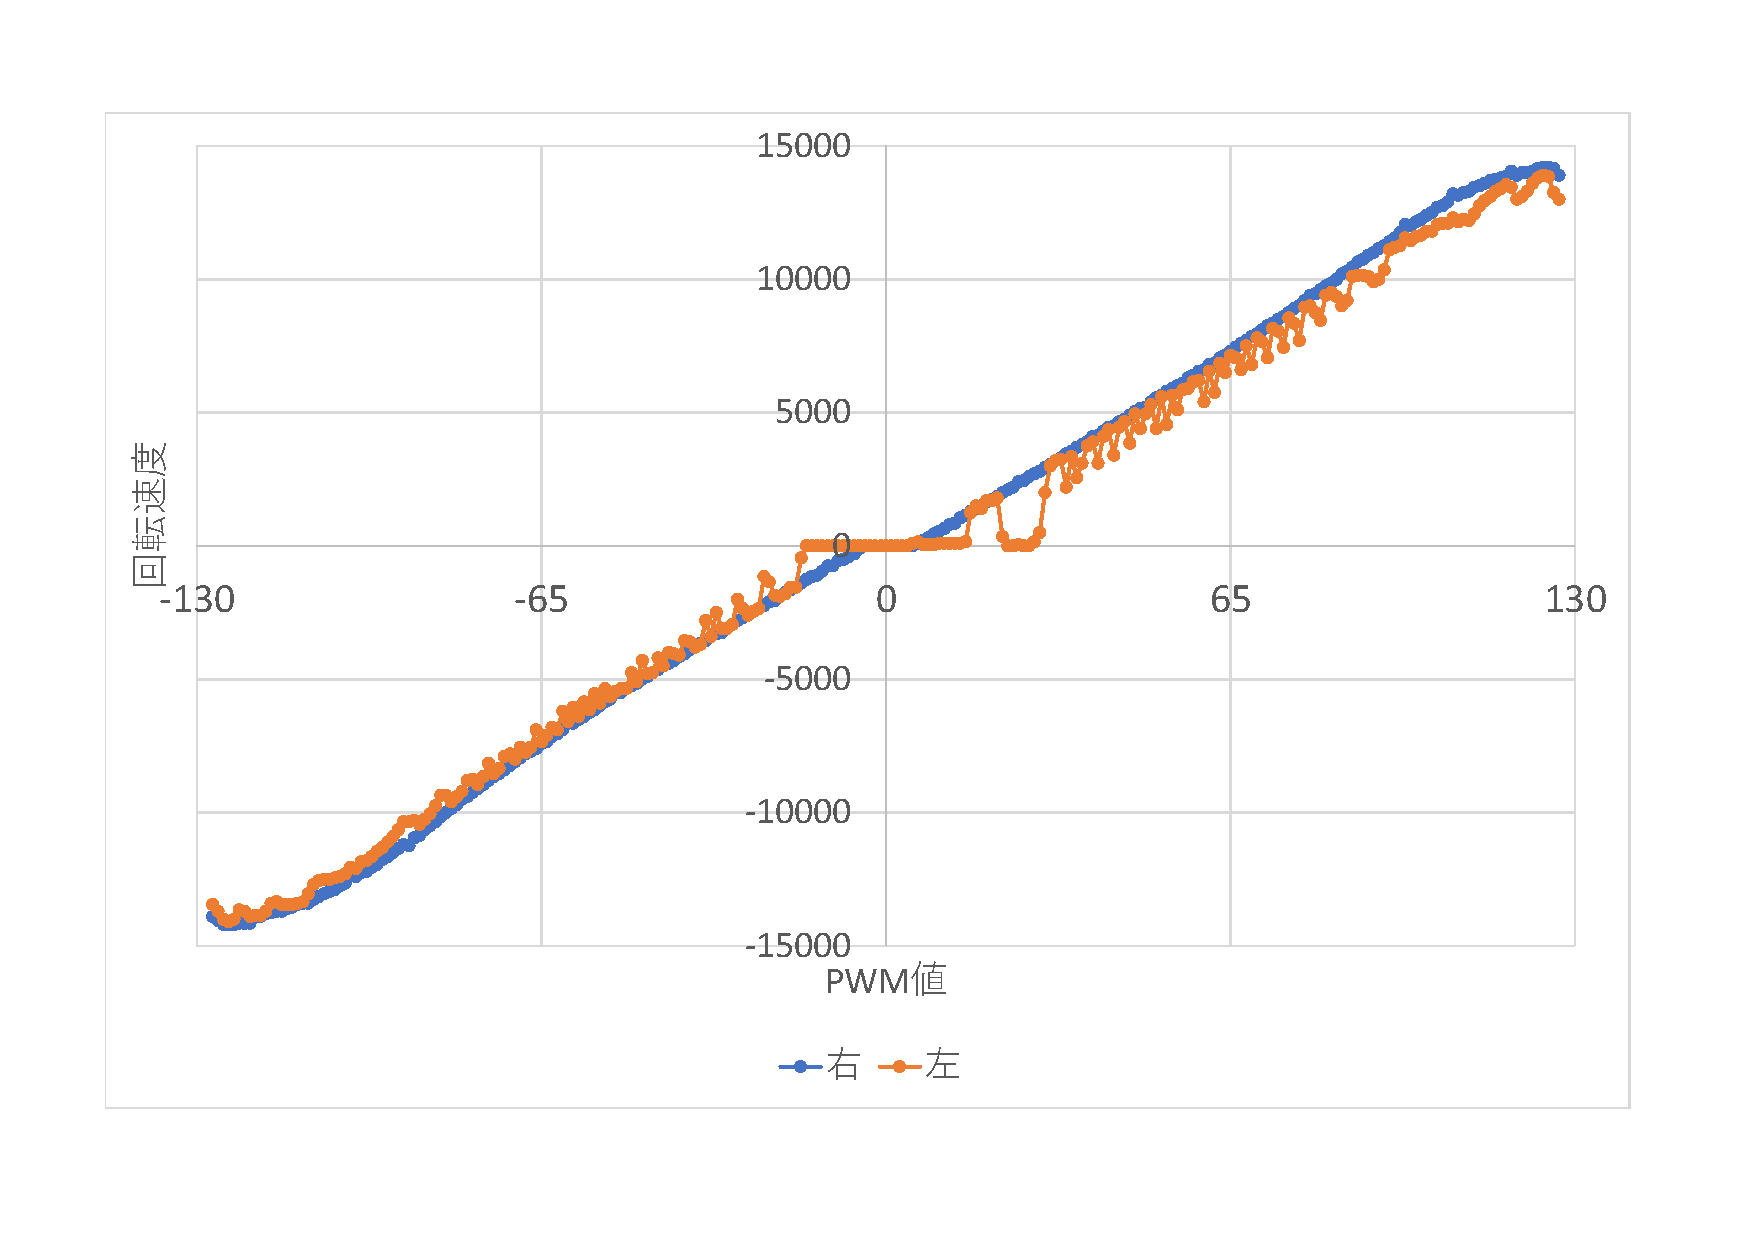
\includegraphics[width=\columnwidth]{img/12.pdf}
  \caption{左右のモータの回転数の特性}
  \label{pwm}
  \end{center}
\end{figure}

\section{演習13}
\subsection{実行プログラム}
実行プログラムをソースコード\ref{s13}に示す。
\begin{lstlisting}[caption=演習13のプログラム,label=s13]
#include <stdio.h>
#include <process.h> /*exit関数の定義*/
#include <dos.h>
#include "v25.h"
#include "ms.h"
  
#define DMAX 500 /*保存するデータ数*/
  
int main(){
  int i;
  int kp, ki_inv;
  int vrefl, vrefr;
  int vl[DMAX], vr[DMAX];
  long ct, ctm, t[DMAX];
  FILE *fp;
  
  ms_init();
  
  kp = ms_read_dip();
  ki_inv = 10000;
  vrefl = 5000;
  vrefr = 5000;
  
  ms_motor_on();
  ms_read_v(&vl[0], &vr[0], &ctm);
  ms_step_res(vrefl, vrefr, kp, ki_inv);
  for(i=1; i<DMAX; i++){
    ms_read_v(&vl[i], &vr[i], &ct);
    t[i] = ct - ctm;
      ms_wait(2);
  }
  ms_motor_off();
  
  if((fp = fopen("data.dat", "wt")) == NULL){
    printf("Can't Open File!!\n");
    exit(1);
  }
  
  for(i=1; i<DMAX; i++){
    fprintf(fp, "%7d %7d %10ld\n", vl[i], vr[i], t[i]);
  }
  fclose(fp);
  return 0;
}
\end{lstlisting}

\subsection{実行結果}
モータのステップ応答(回転速度と時間)
をデータファイルに保存する。
比例フィードバック係数$k_p$をスイッチ値(0\verb|~|15)を変化させた時の
応答グラフを図\ref{im0}\verb|~|\ref{im15}に示す。
なお、$k_p$の値は\tsuyo{7}で安定とした。
$k_p = 0 ~ 2$の場合、ロボットは前進しない。
\begin{figure}[H]
  \begin{center}
  \subfigure[$k_p=0$]{
  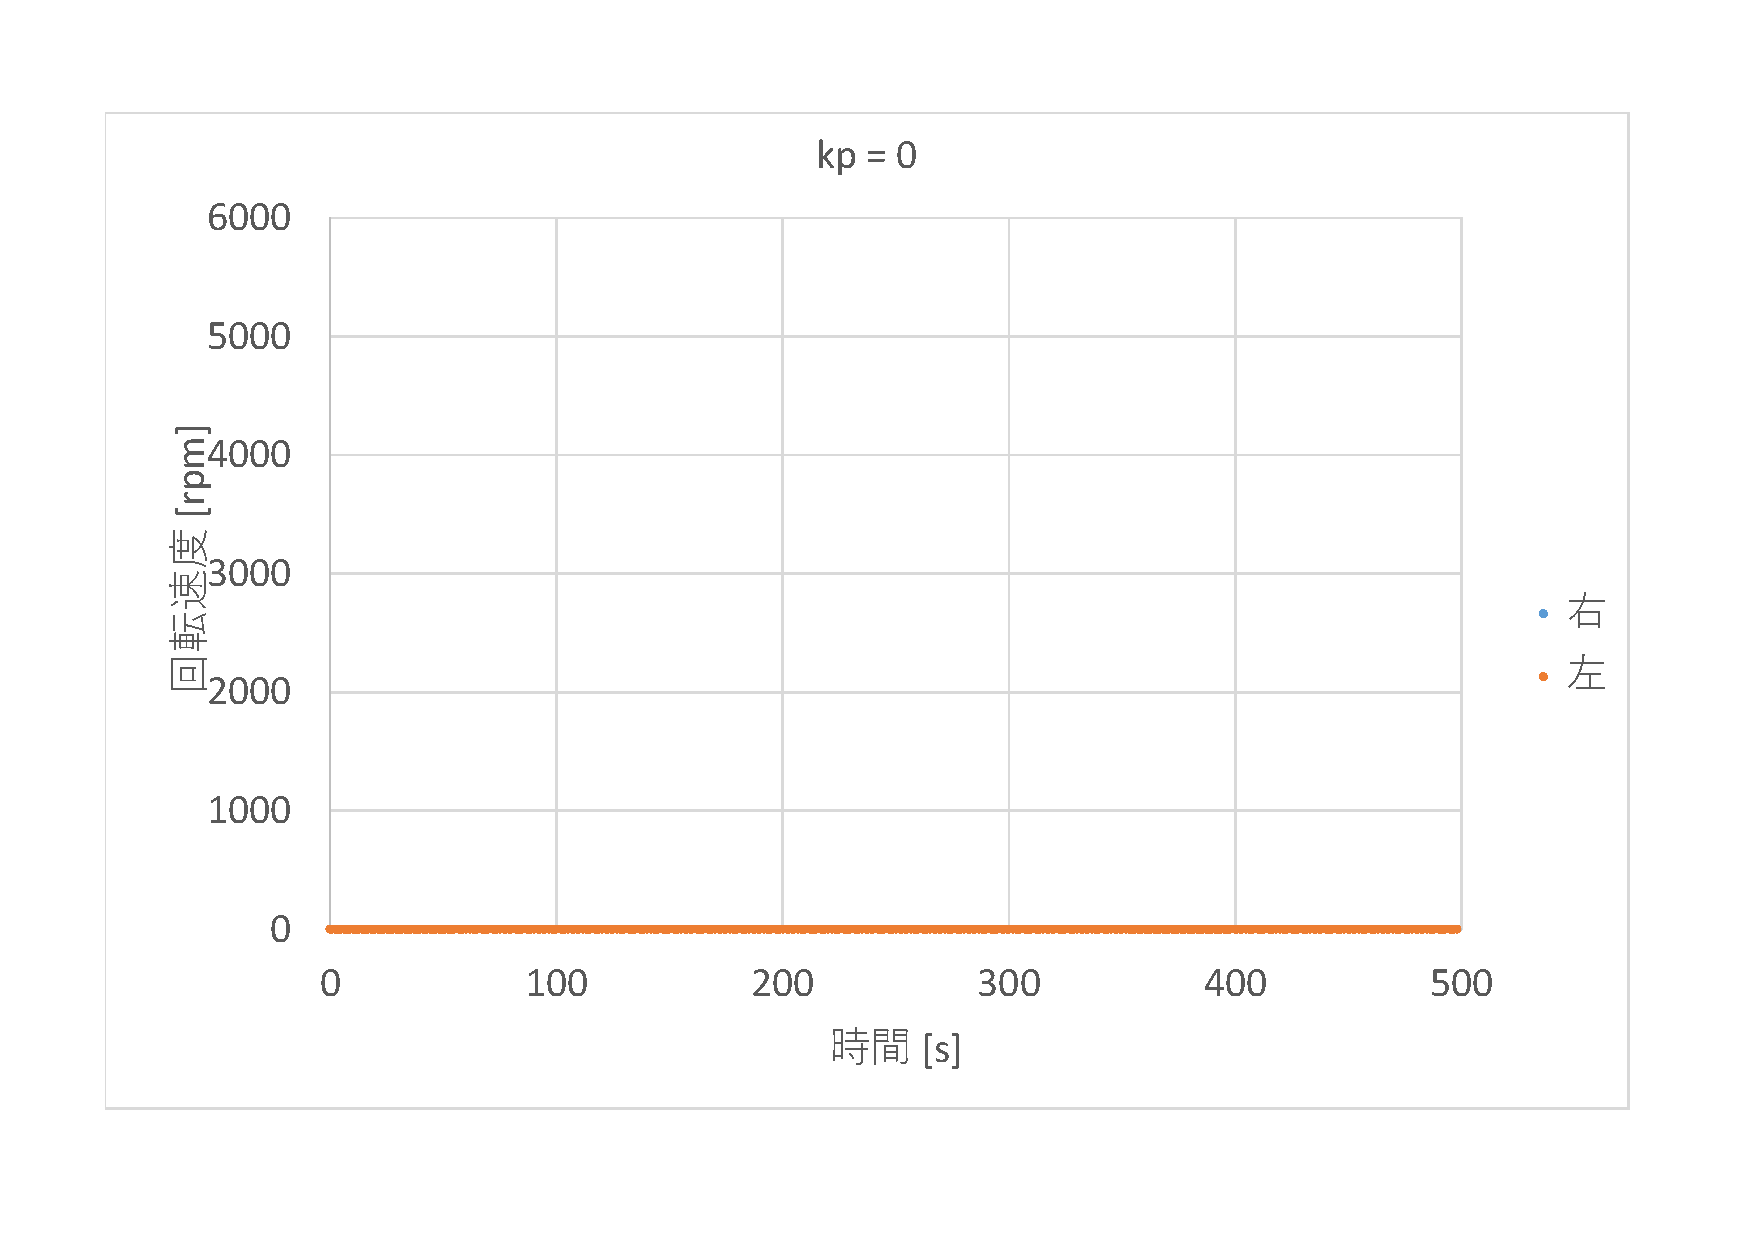
\includegraphics[width=\columnwidth]{img/13/DATA0.pdf}
  \label{im0}
  }
  \subfigure[$k_p=1$]{
  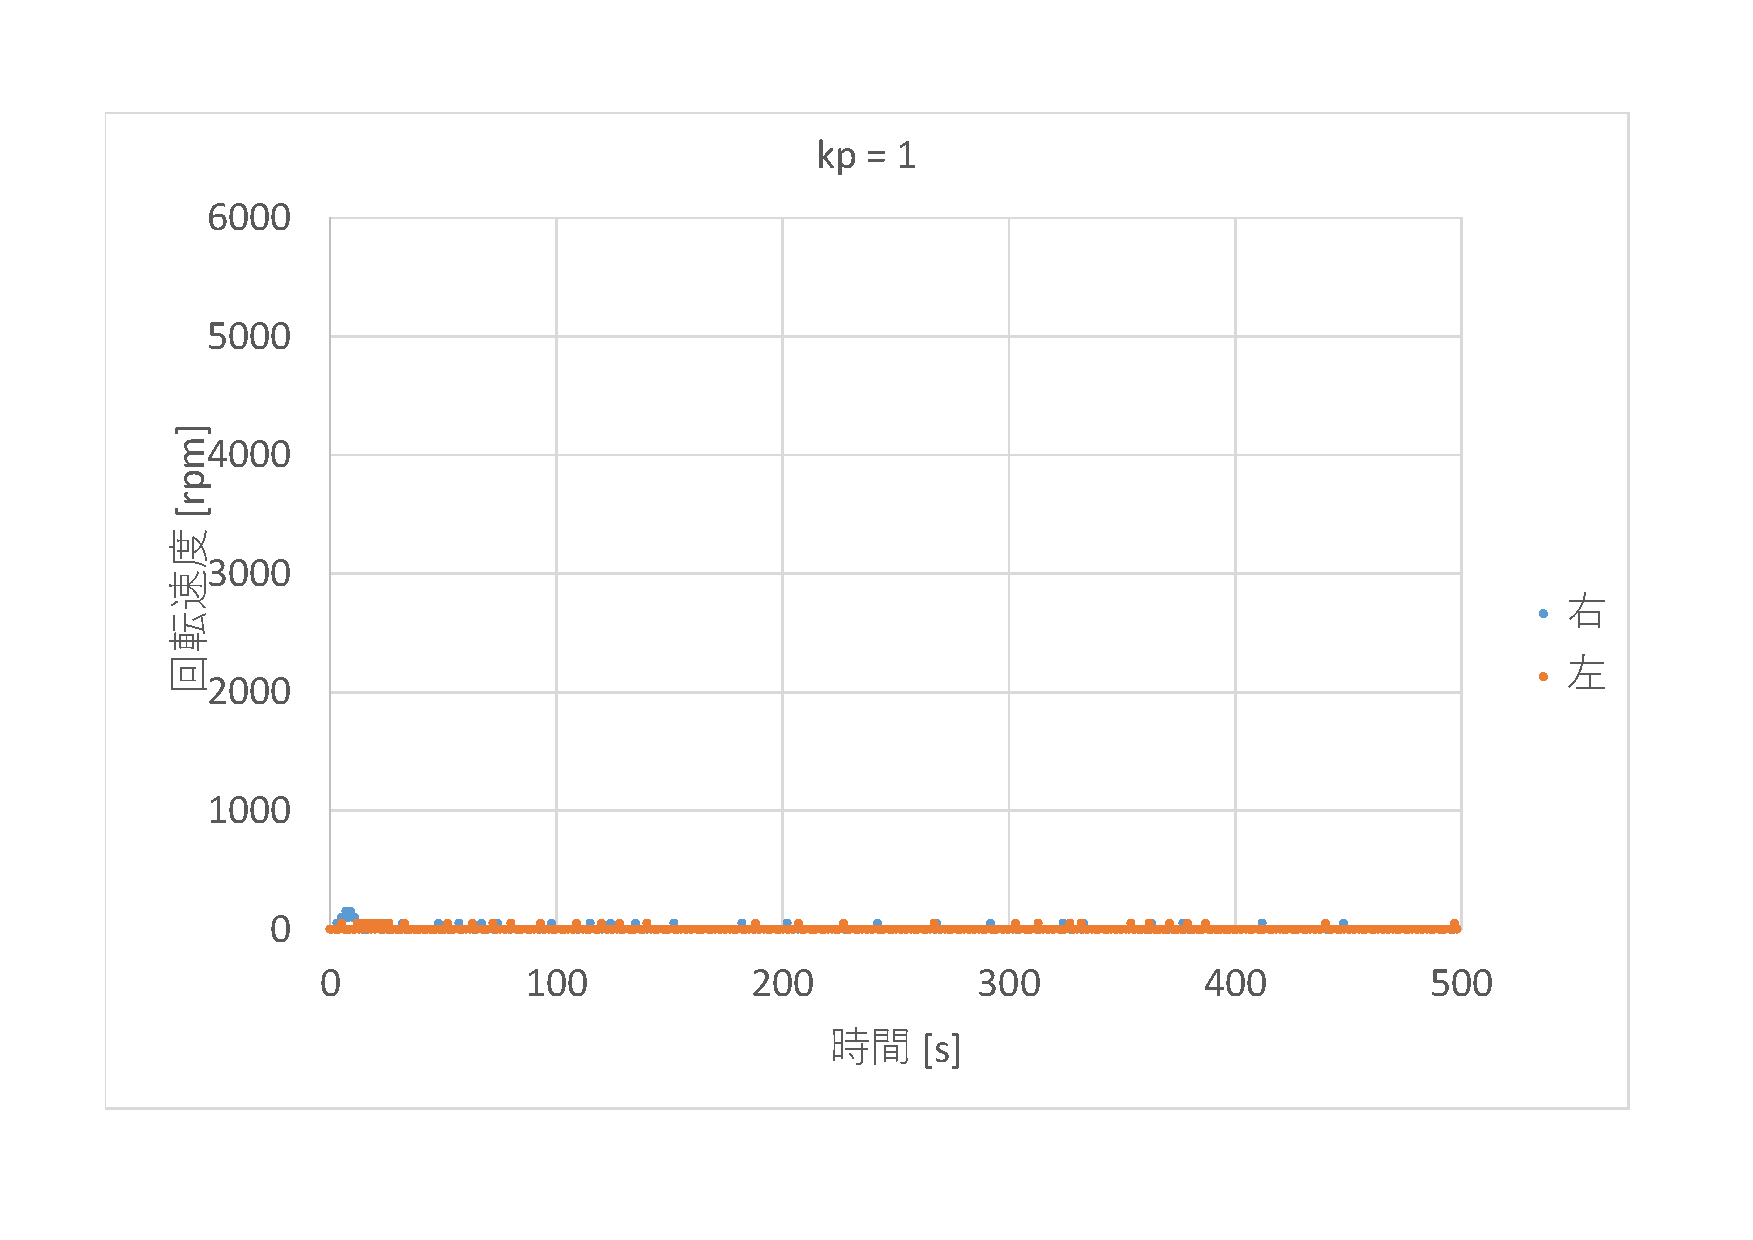
\includegraphics[width=\columnwidth]{img/13/DATA1.pdf}
  \label{im1}
  }
  \caption{ステップ応答のグラフ}
  \end{center}
\end{figure}

\begin{figure}[H]
  \begin{center}
  \subfigure[$k_p=2$]{
  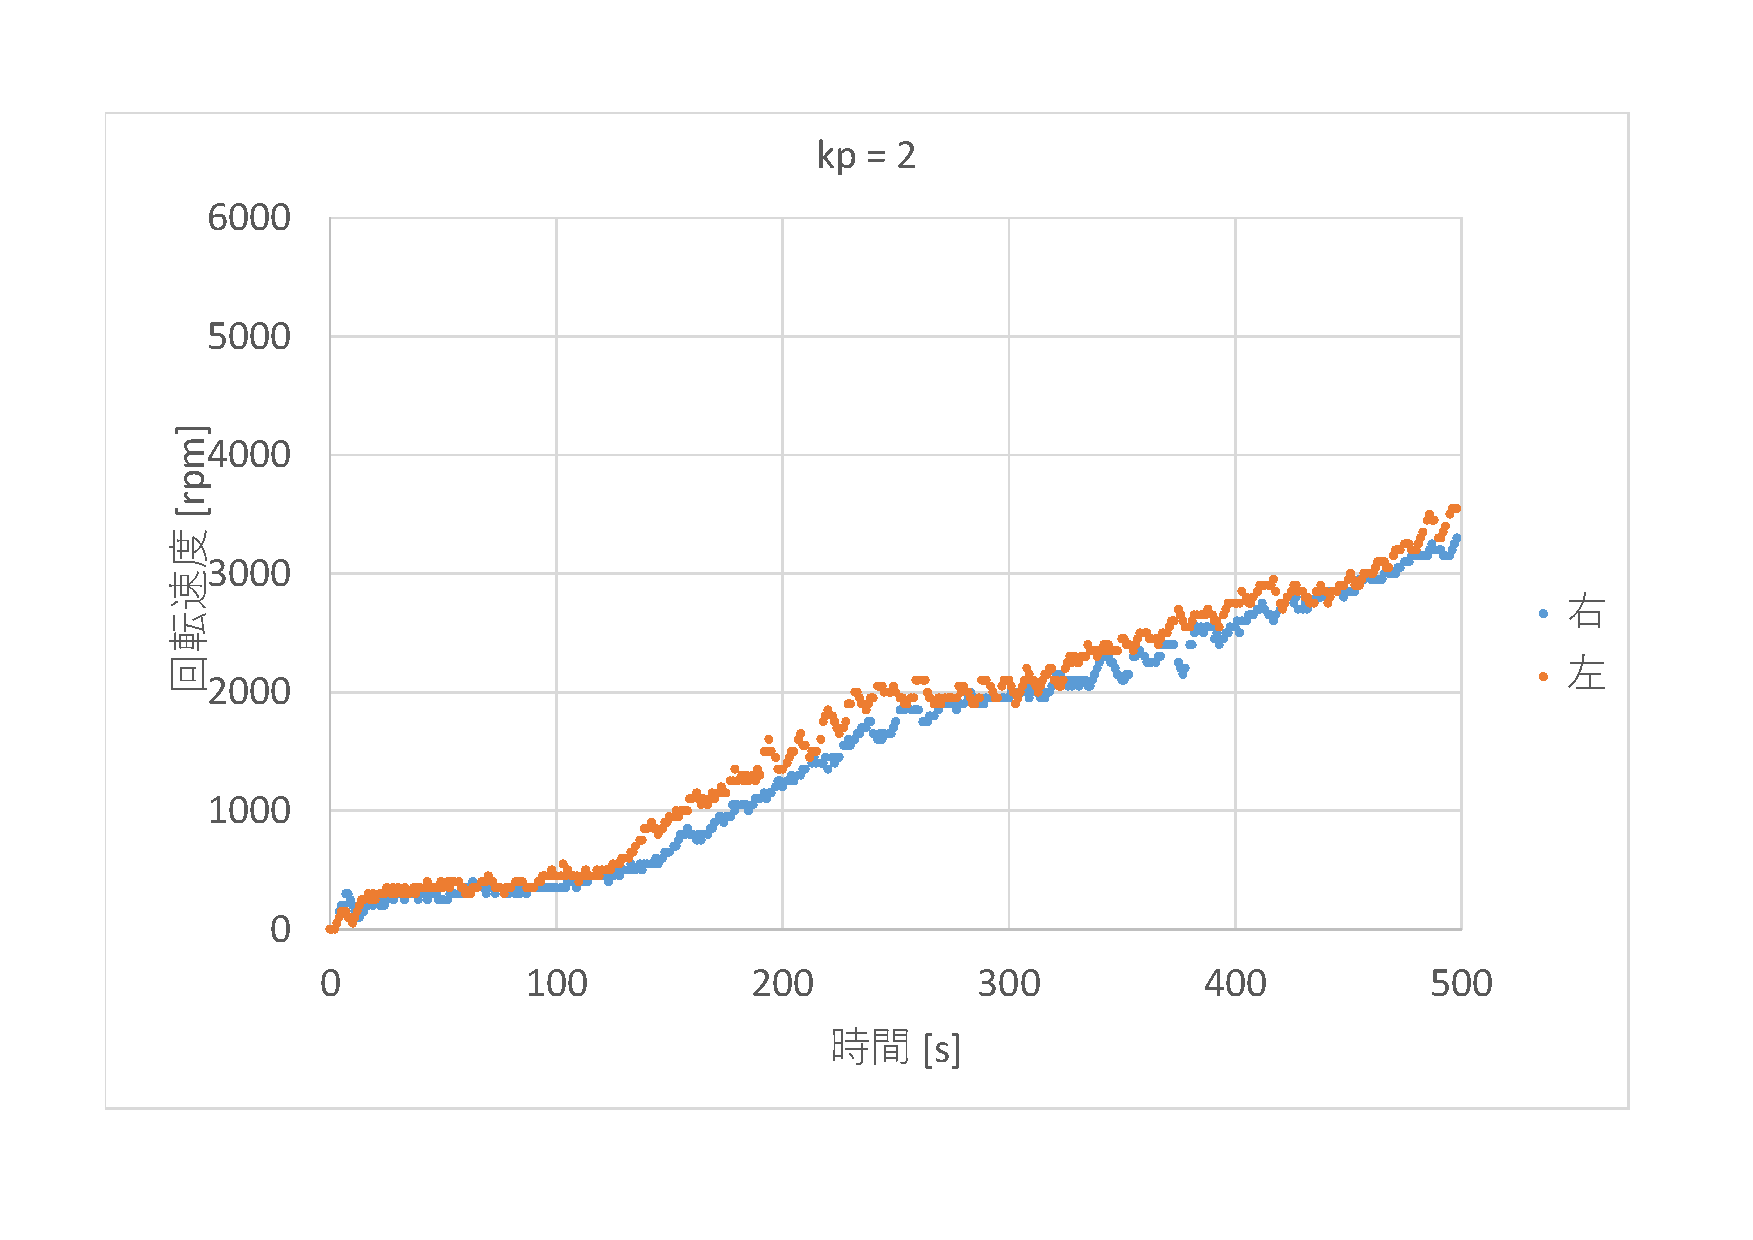
\includegraphics[width=\columnwidth]{img/13/DATA2.pdf}
  \label{im2}
  }
  \subfigure[$k_p=3$]{
  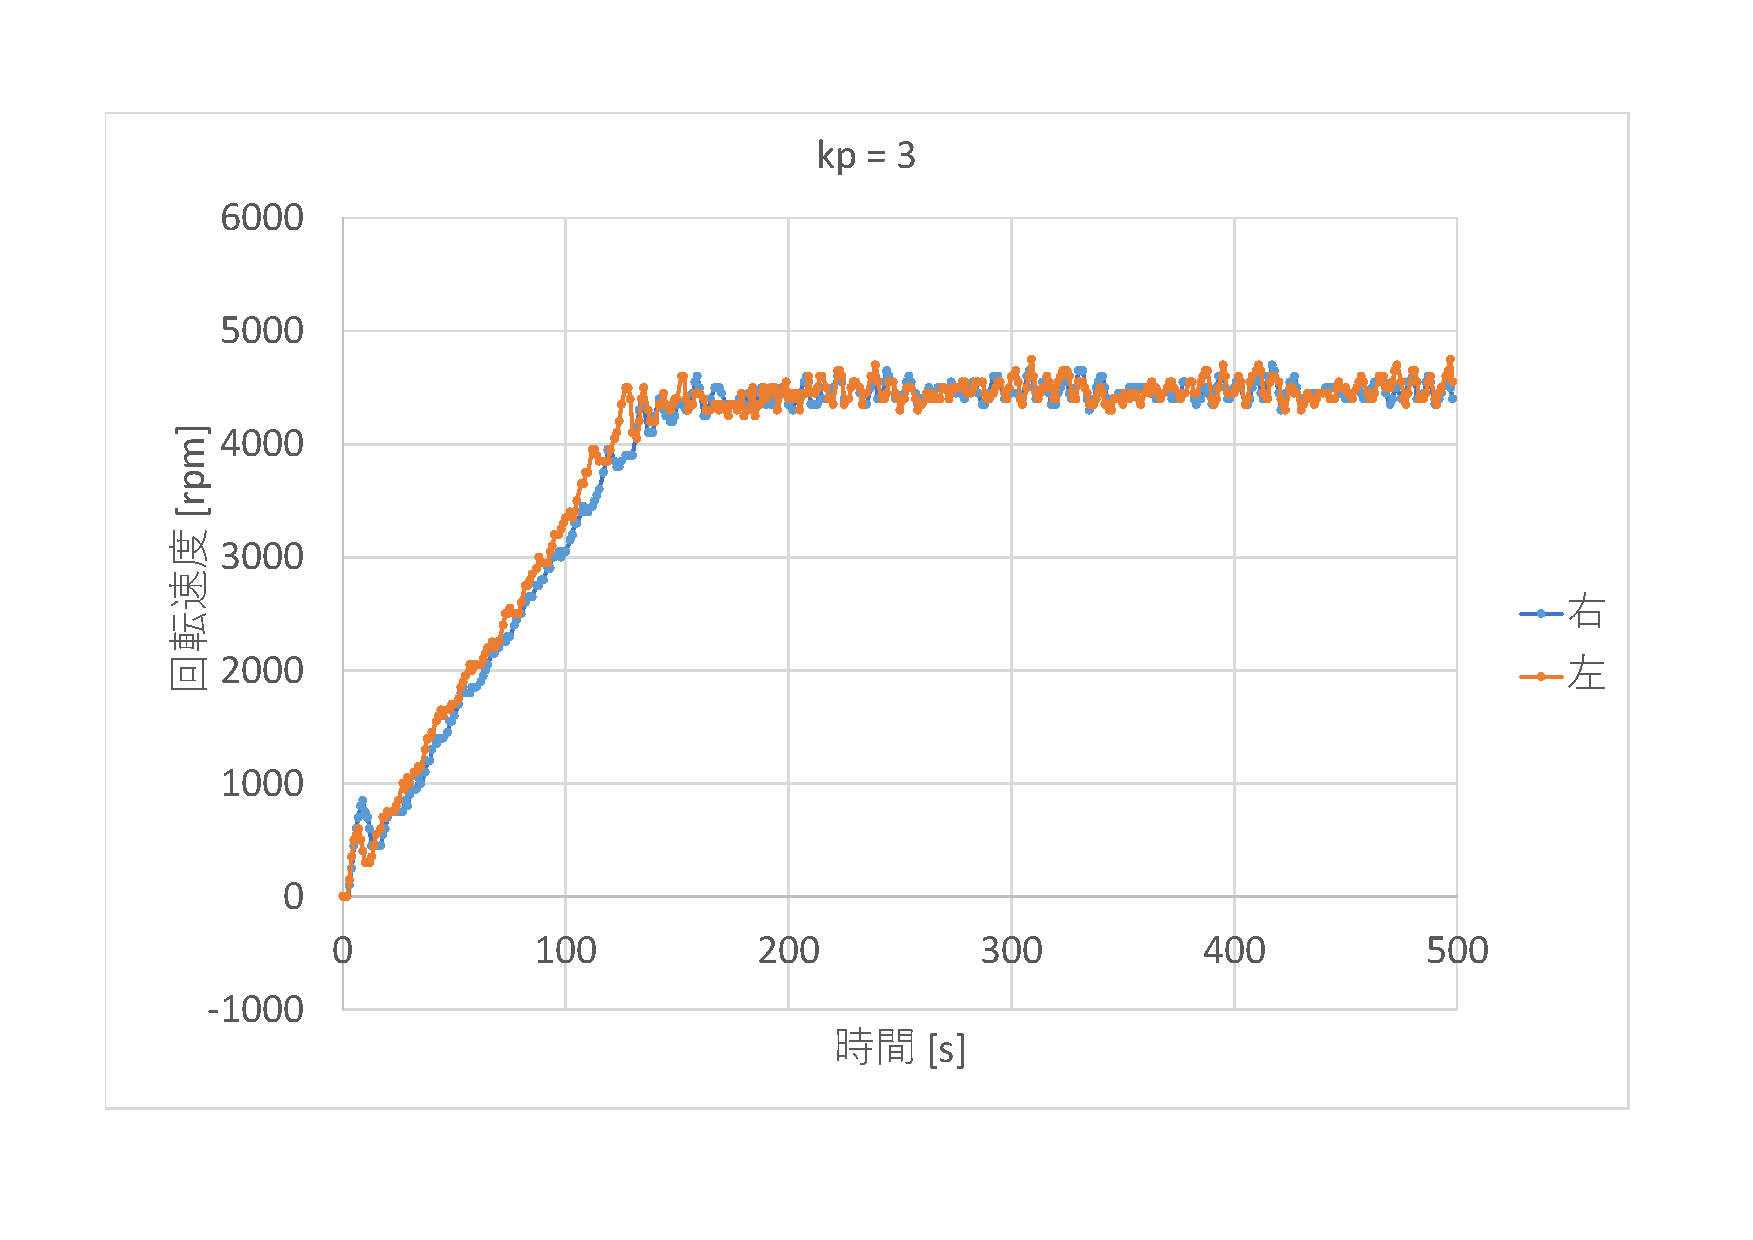
\includegraphics[width=\columnwidth]{img/13/DATA3.pdf}
  \label{im3}
  }
  \caption{ステップ応答のグラフ}
  \end{center}
\end{figure}

\begin{figure}[H]
  \begin{center}
  \subfigure[$k_p=4$]{
  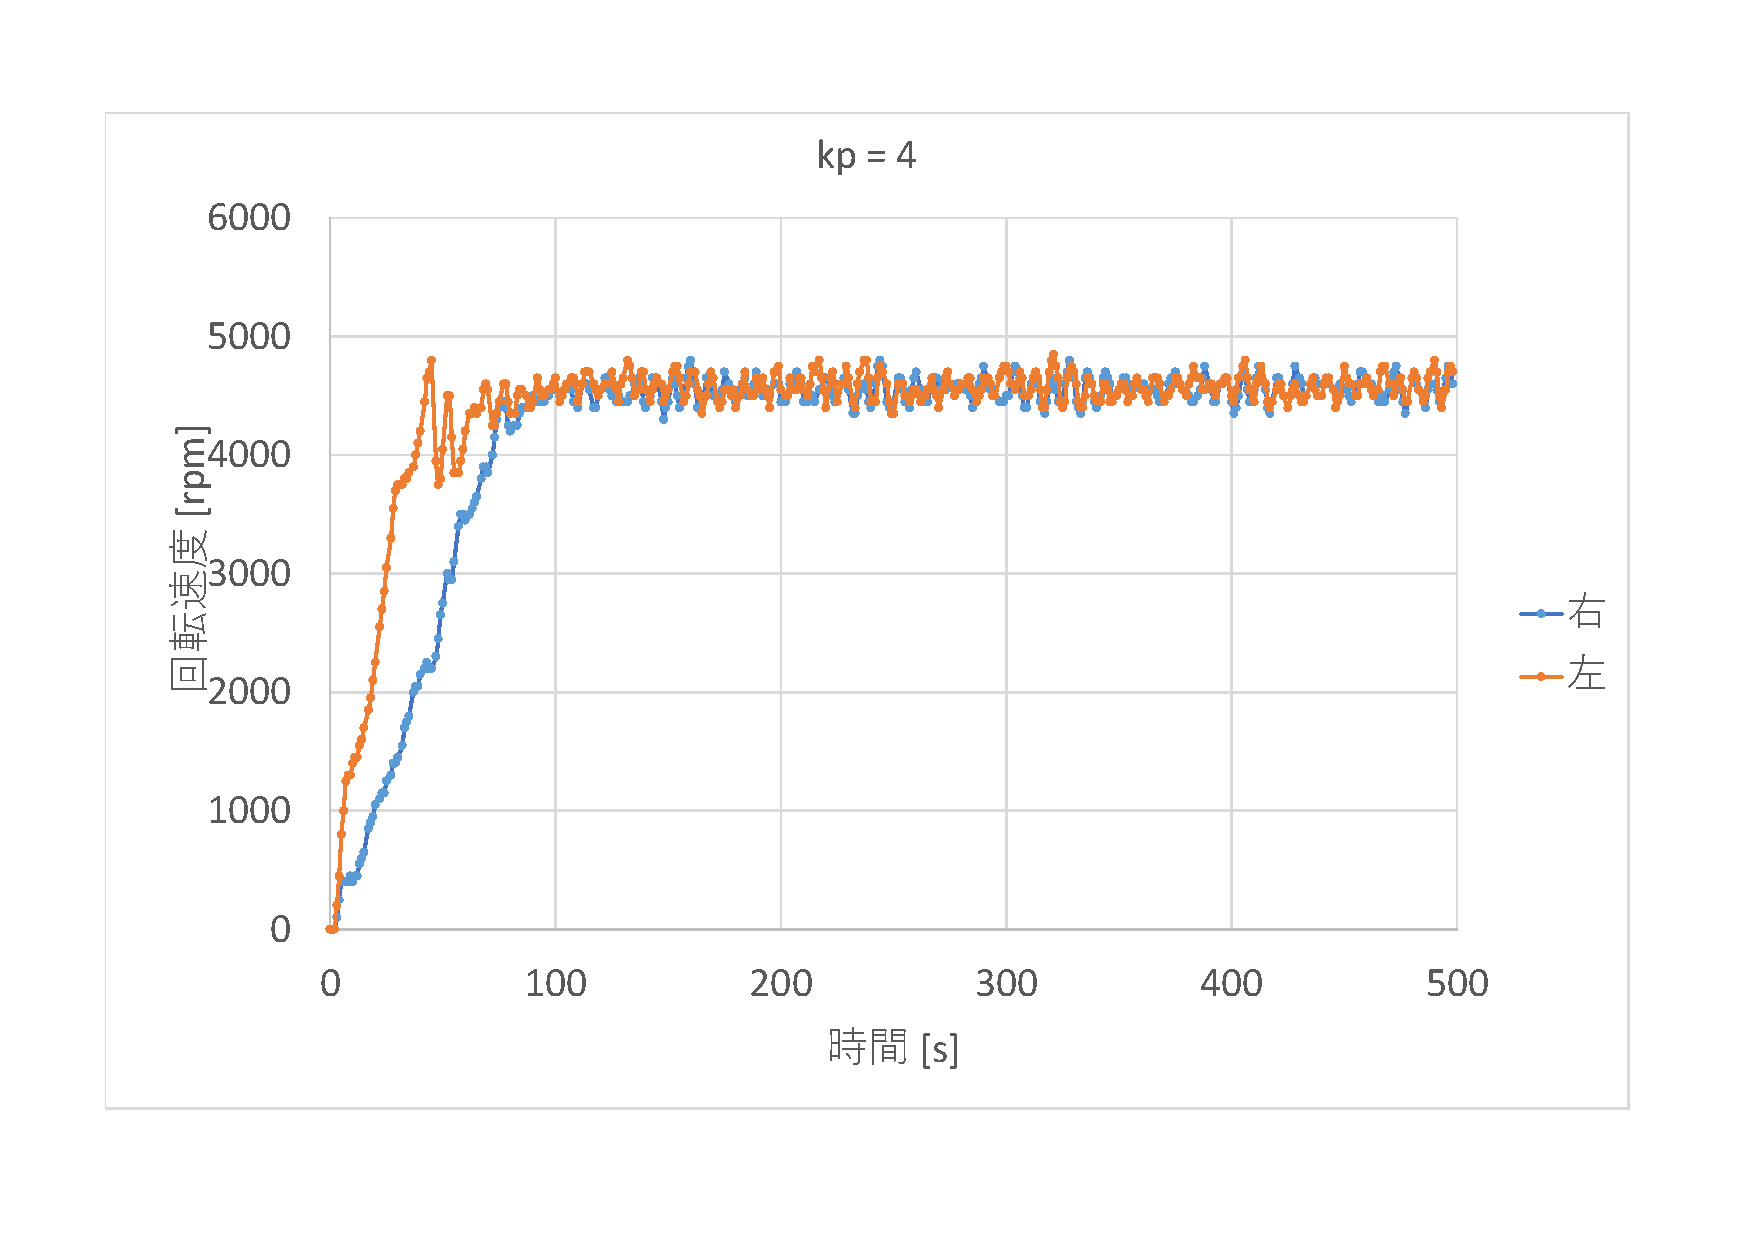
\includegraphics[width=\columnwidth]{img/13/DATA4.pdf}
  \label{im4}
  }
  \subfigure[$k_p=5$]{
  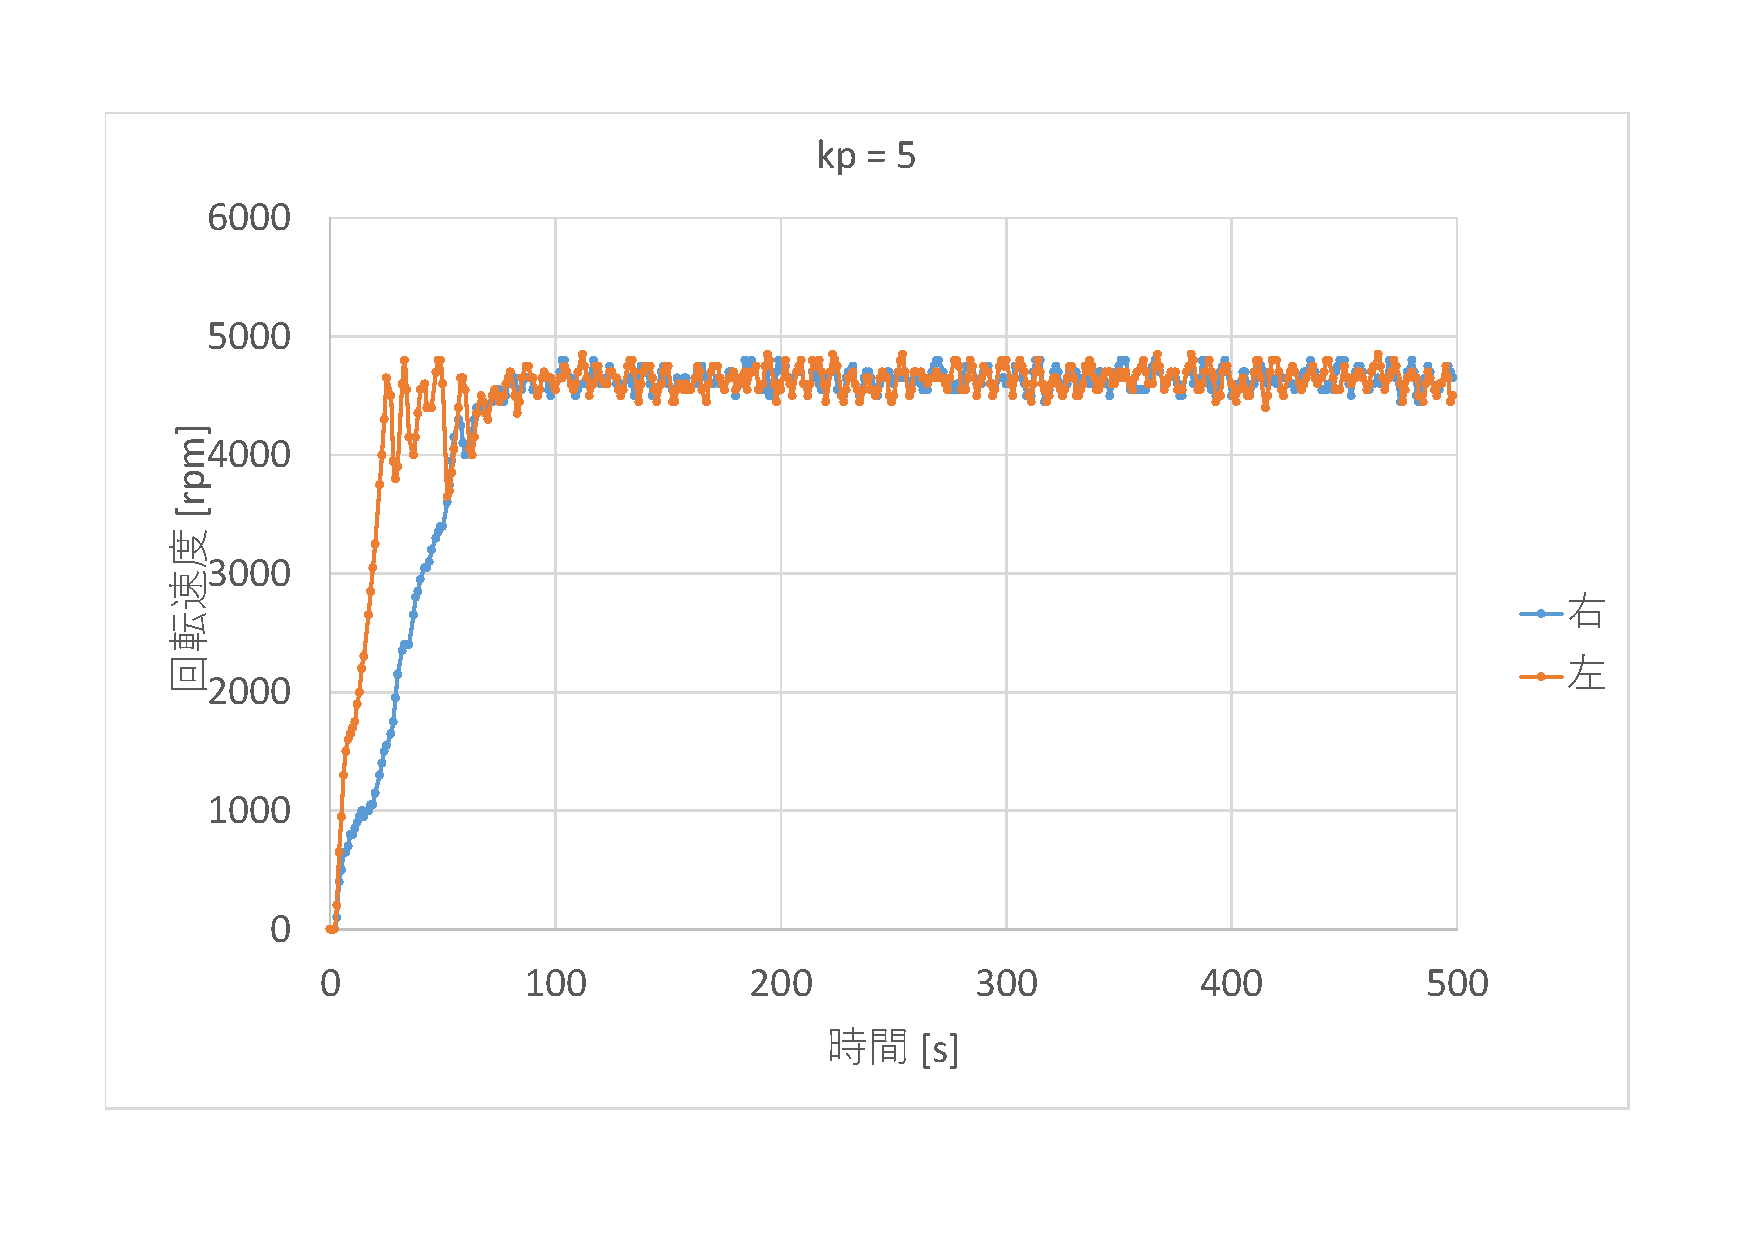
\includegraphics[width=\columnwidth]{img/13/DATA5.pdf}
  \label{im5}
  }
  \caption{ステップ応答のグラフ}
  \end{center}
\end{figure}

\begin{figure}[H]
  \begin{center}  
  \subfigure[$k_p=6$]{
  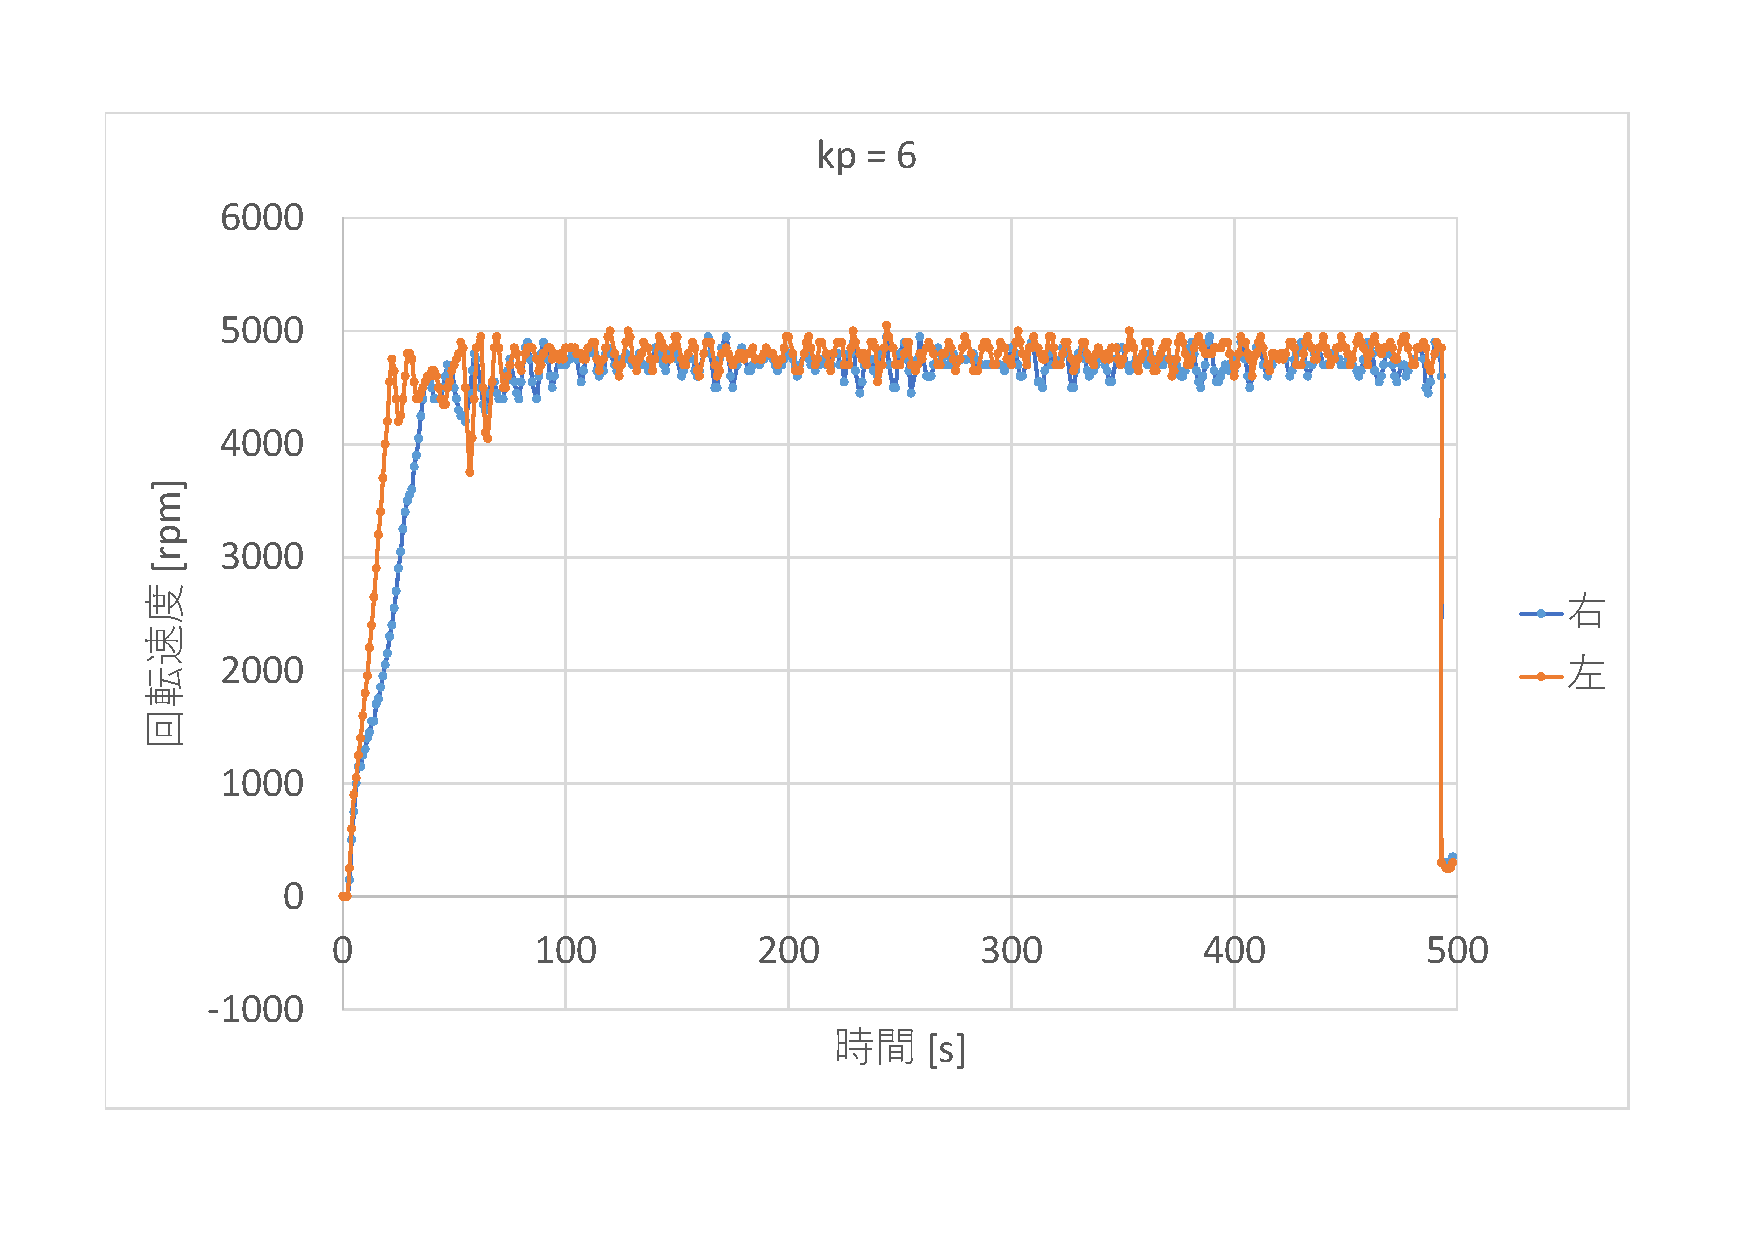
\includegraphics[width=\columnwidth]{img/13/DATA6.pdf}
  \label{im6}
  }
  \subfigure[$k_p=7$]{
  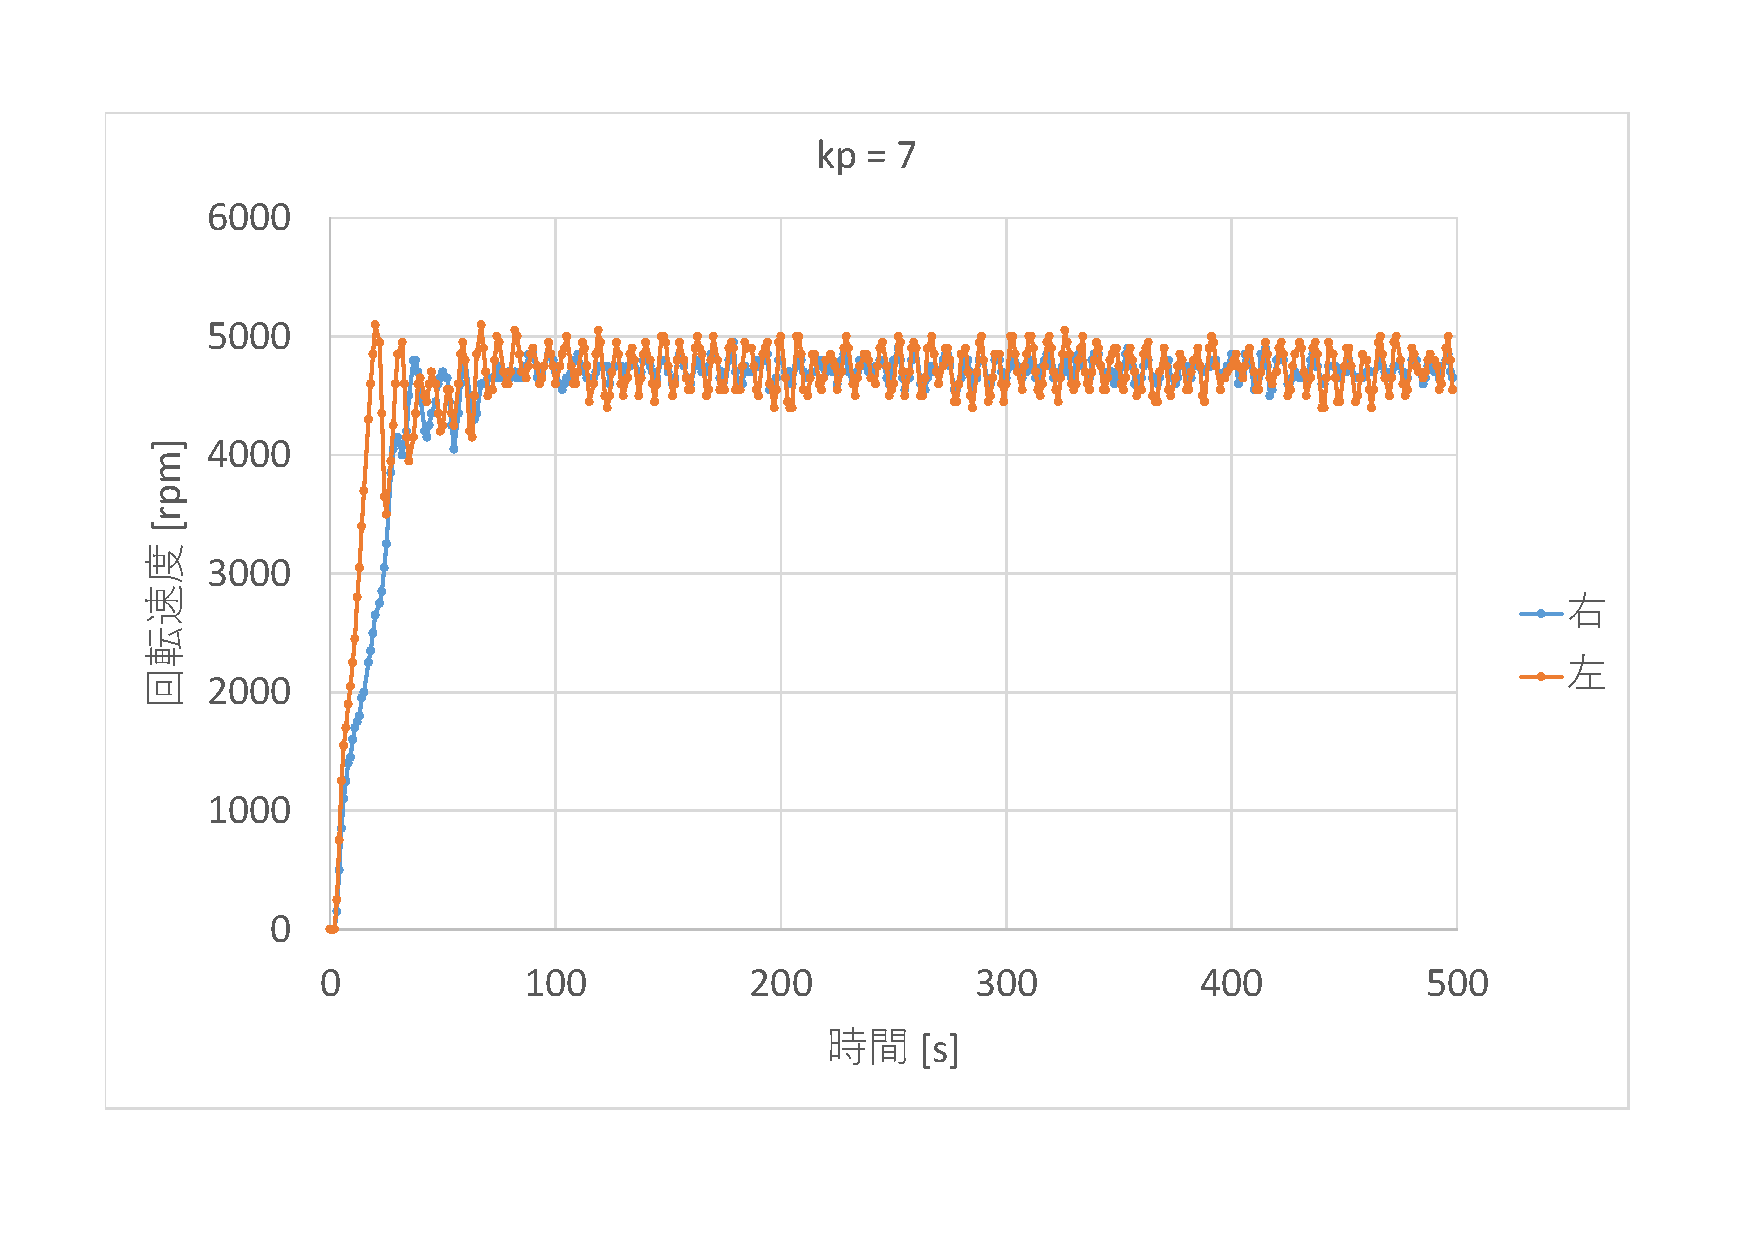
\includegraphics[width=\columnwidth]{img/13/DATA7.pdf}
  \label{im7}
  }
  \caption{ステップ応答のグラフ}
  \end{center}
\end{figure}

\begin{figure}[H]
  \begin{center}
  \subfigure[$k_p=8$]{
  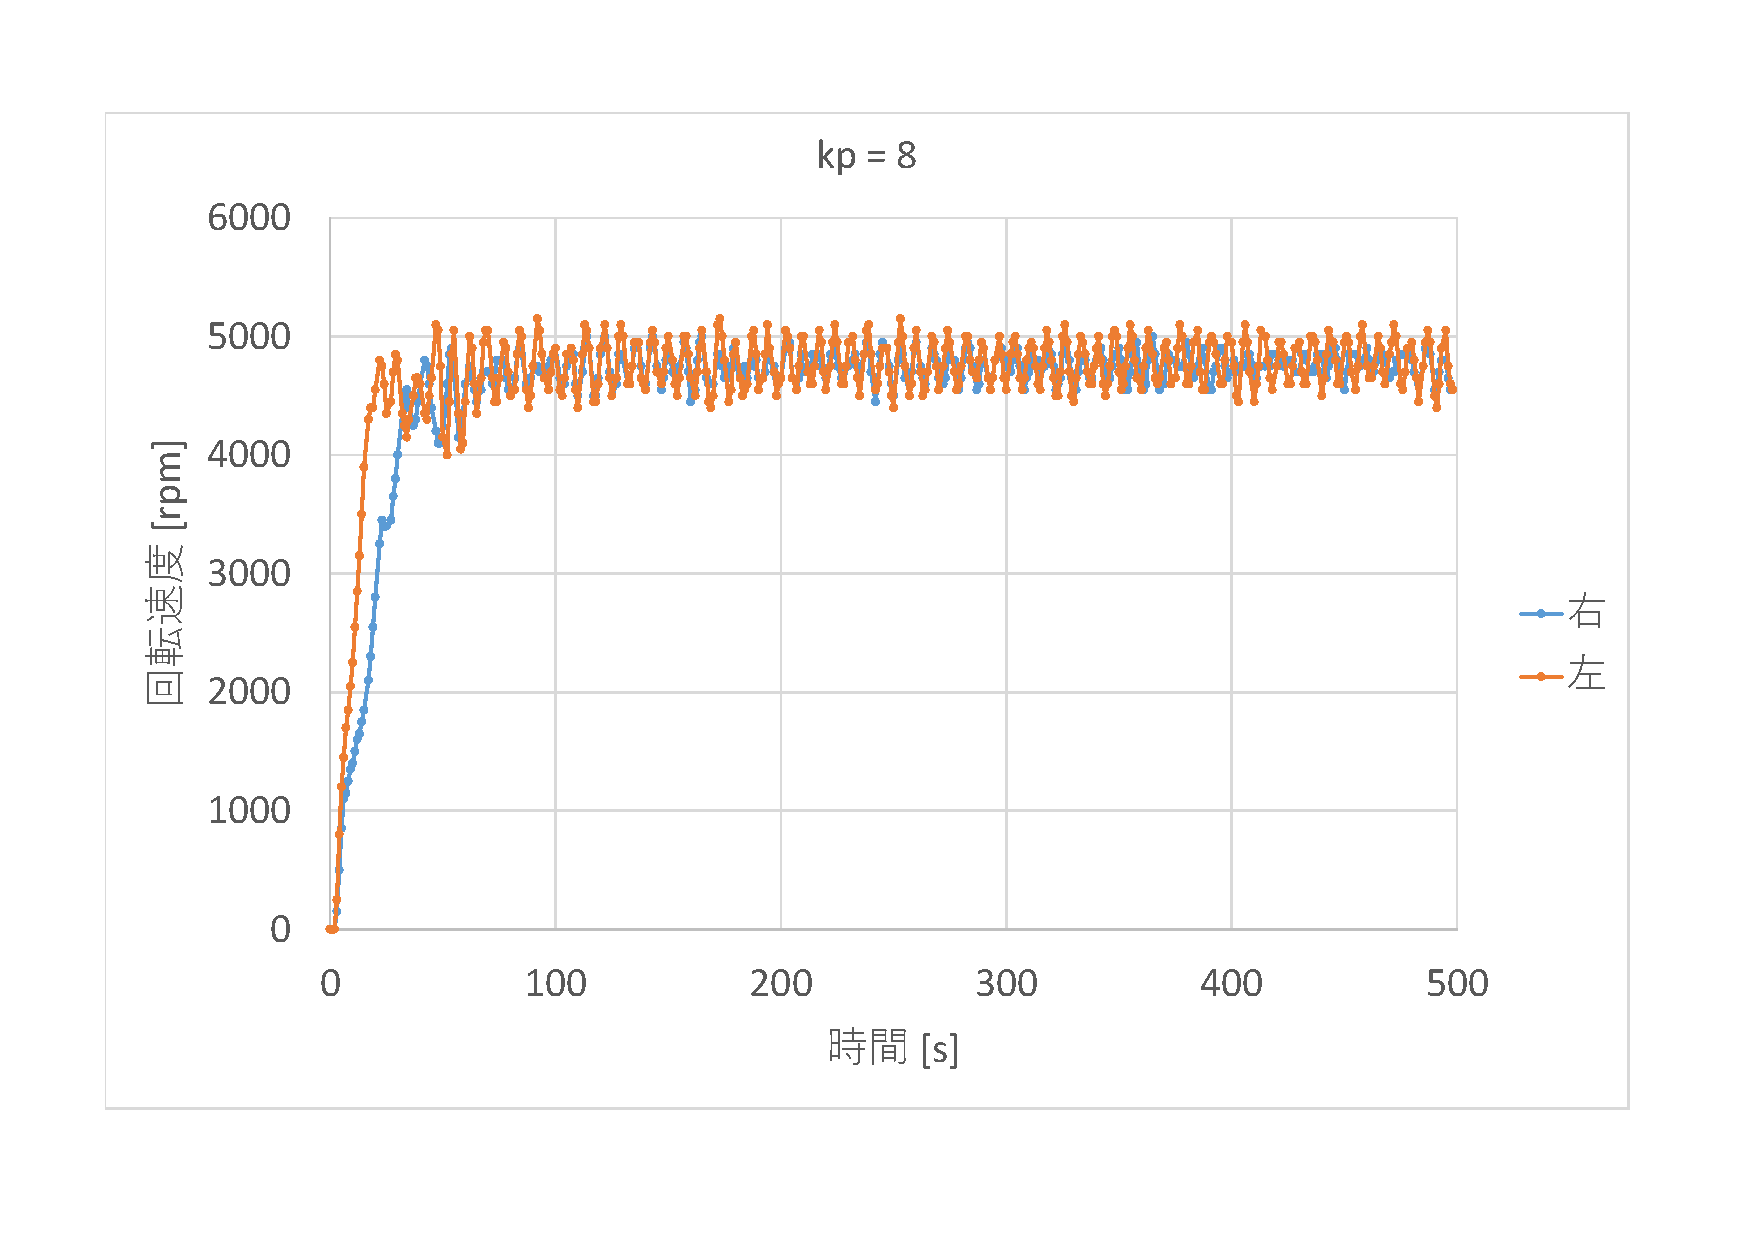
\includegraphics[width=\columnwidth]{img/13/DATA8.pdf}
  \label{im8}
  }
  \subfigure[$k_p=9$]{
  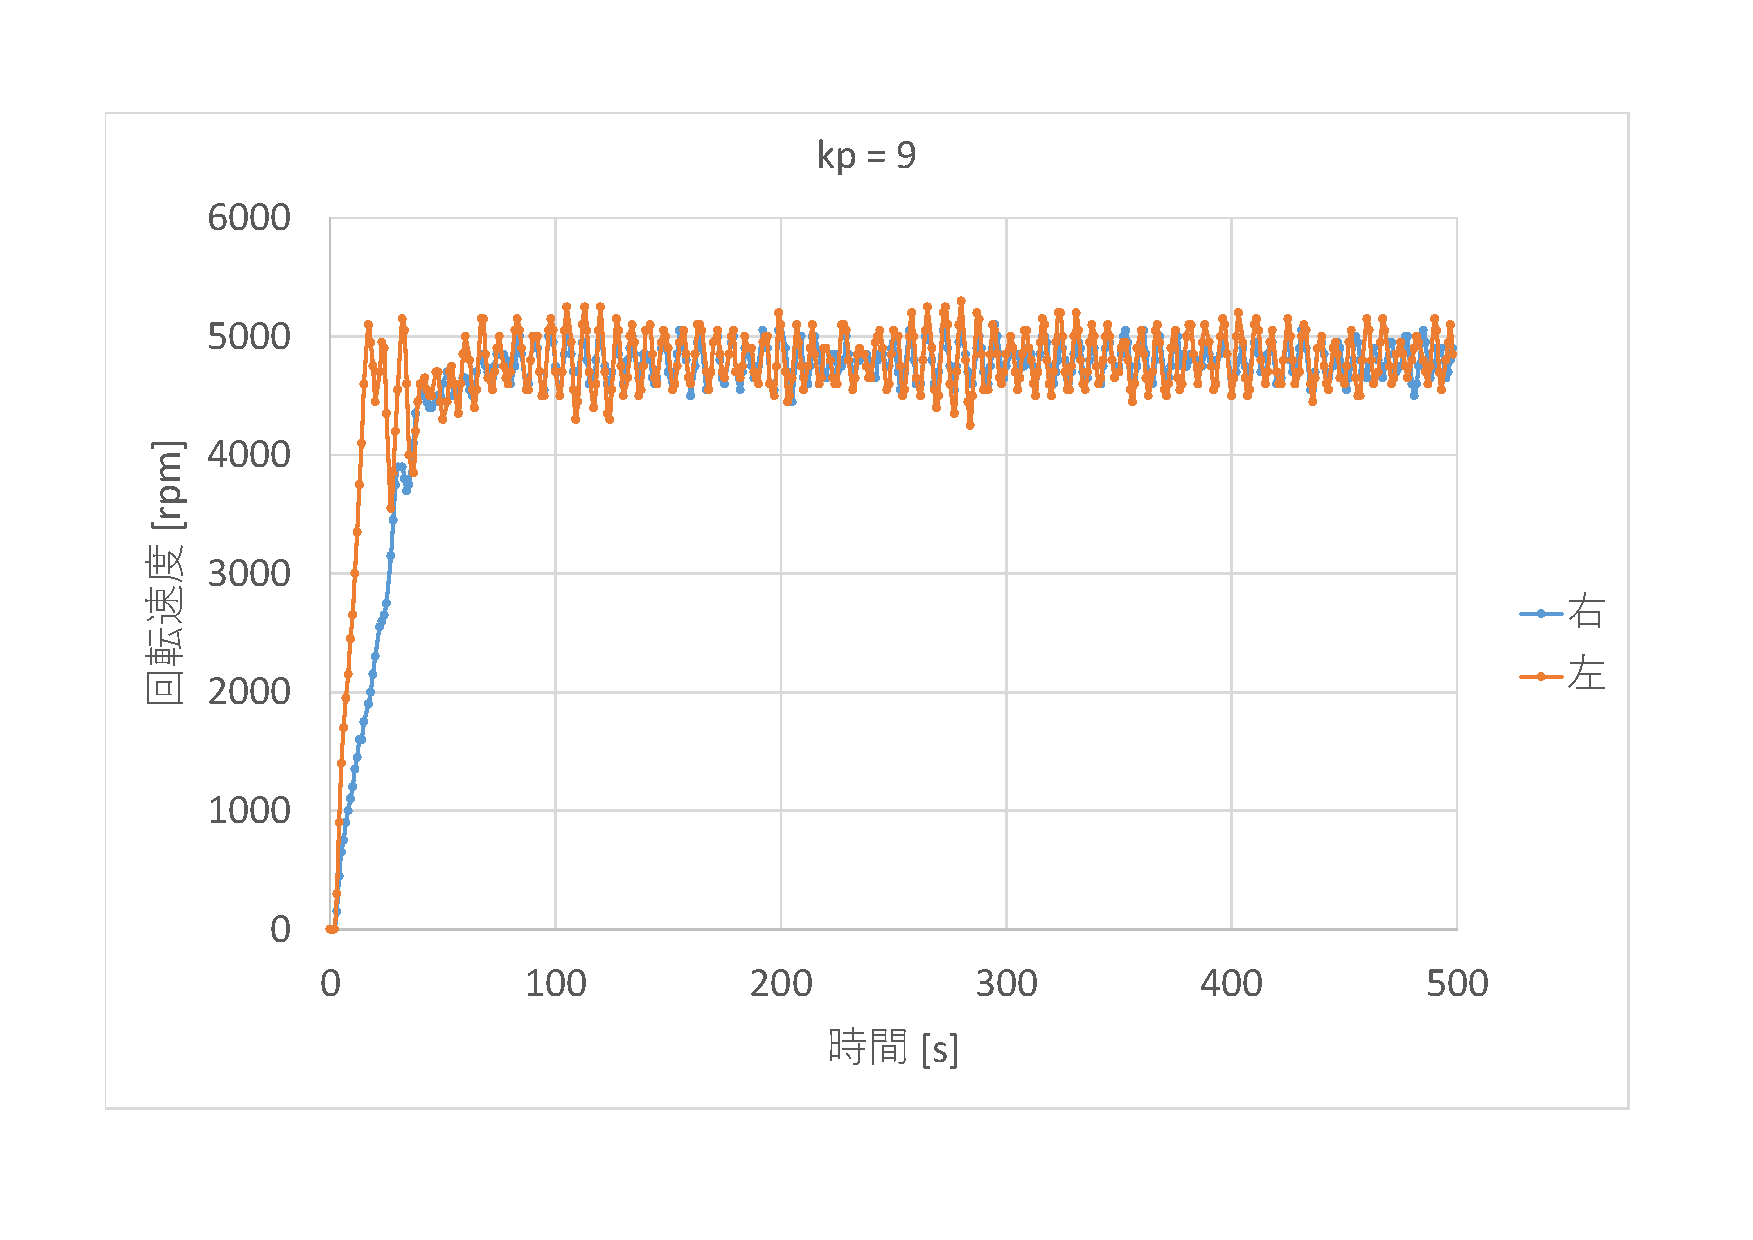
\includegraphics[width=\columnwidth]{img/13/DATA9.pdf}
  \label{im9}
  }
  \caption{ステップ応答のグラフ}
  \end{center}
\end{figure}

\begin{figure}[H]
  \begin{center}
  \subfigure[$k_p=10$]{
  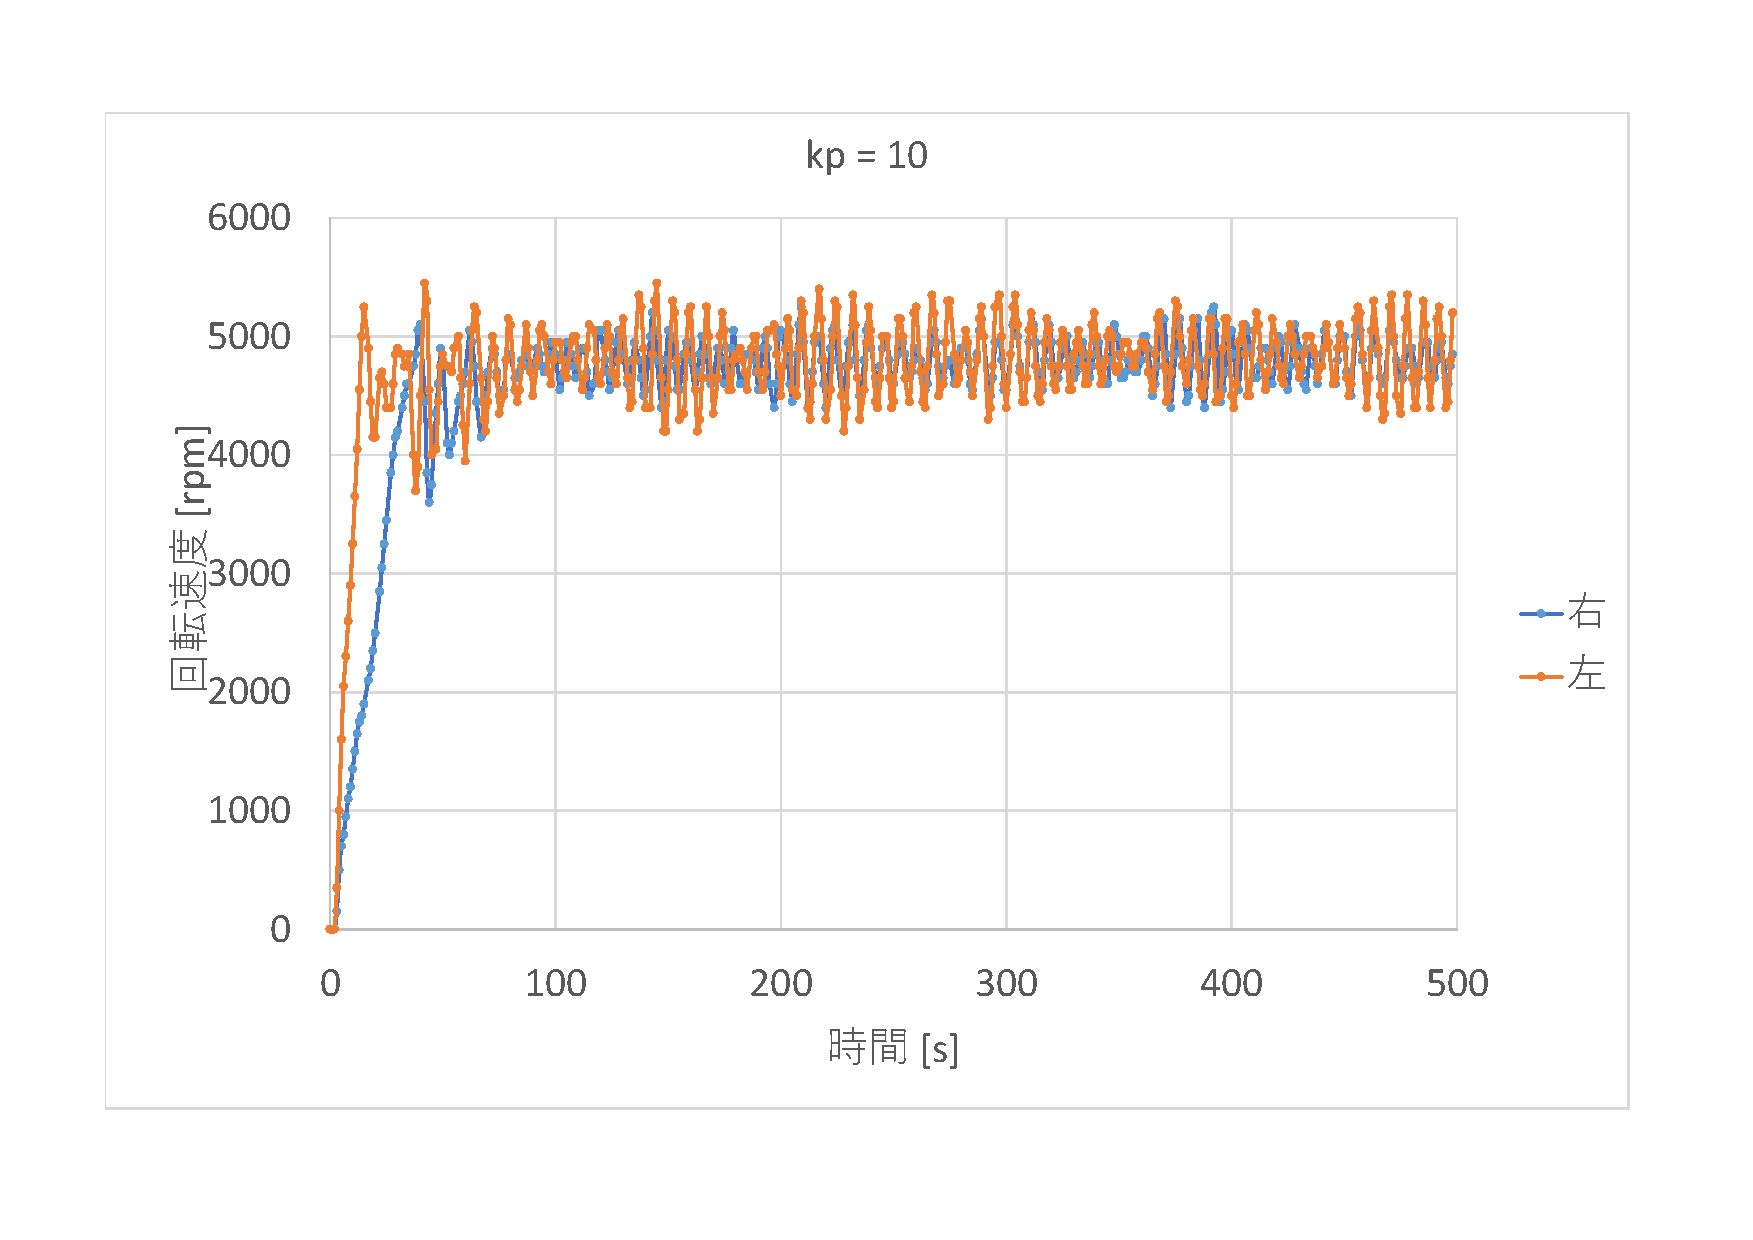
\includegraphics[width=\columnwidth]{img/13/DATA10.pdf}
  \label{im10}
  }
  \subfigure[$k_p=11$]{
  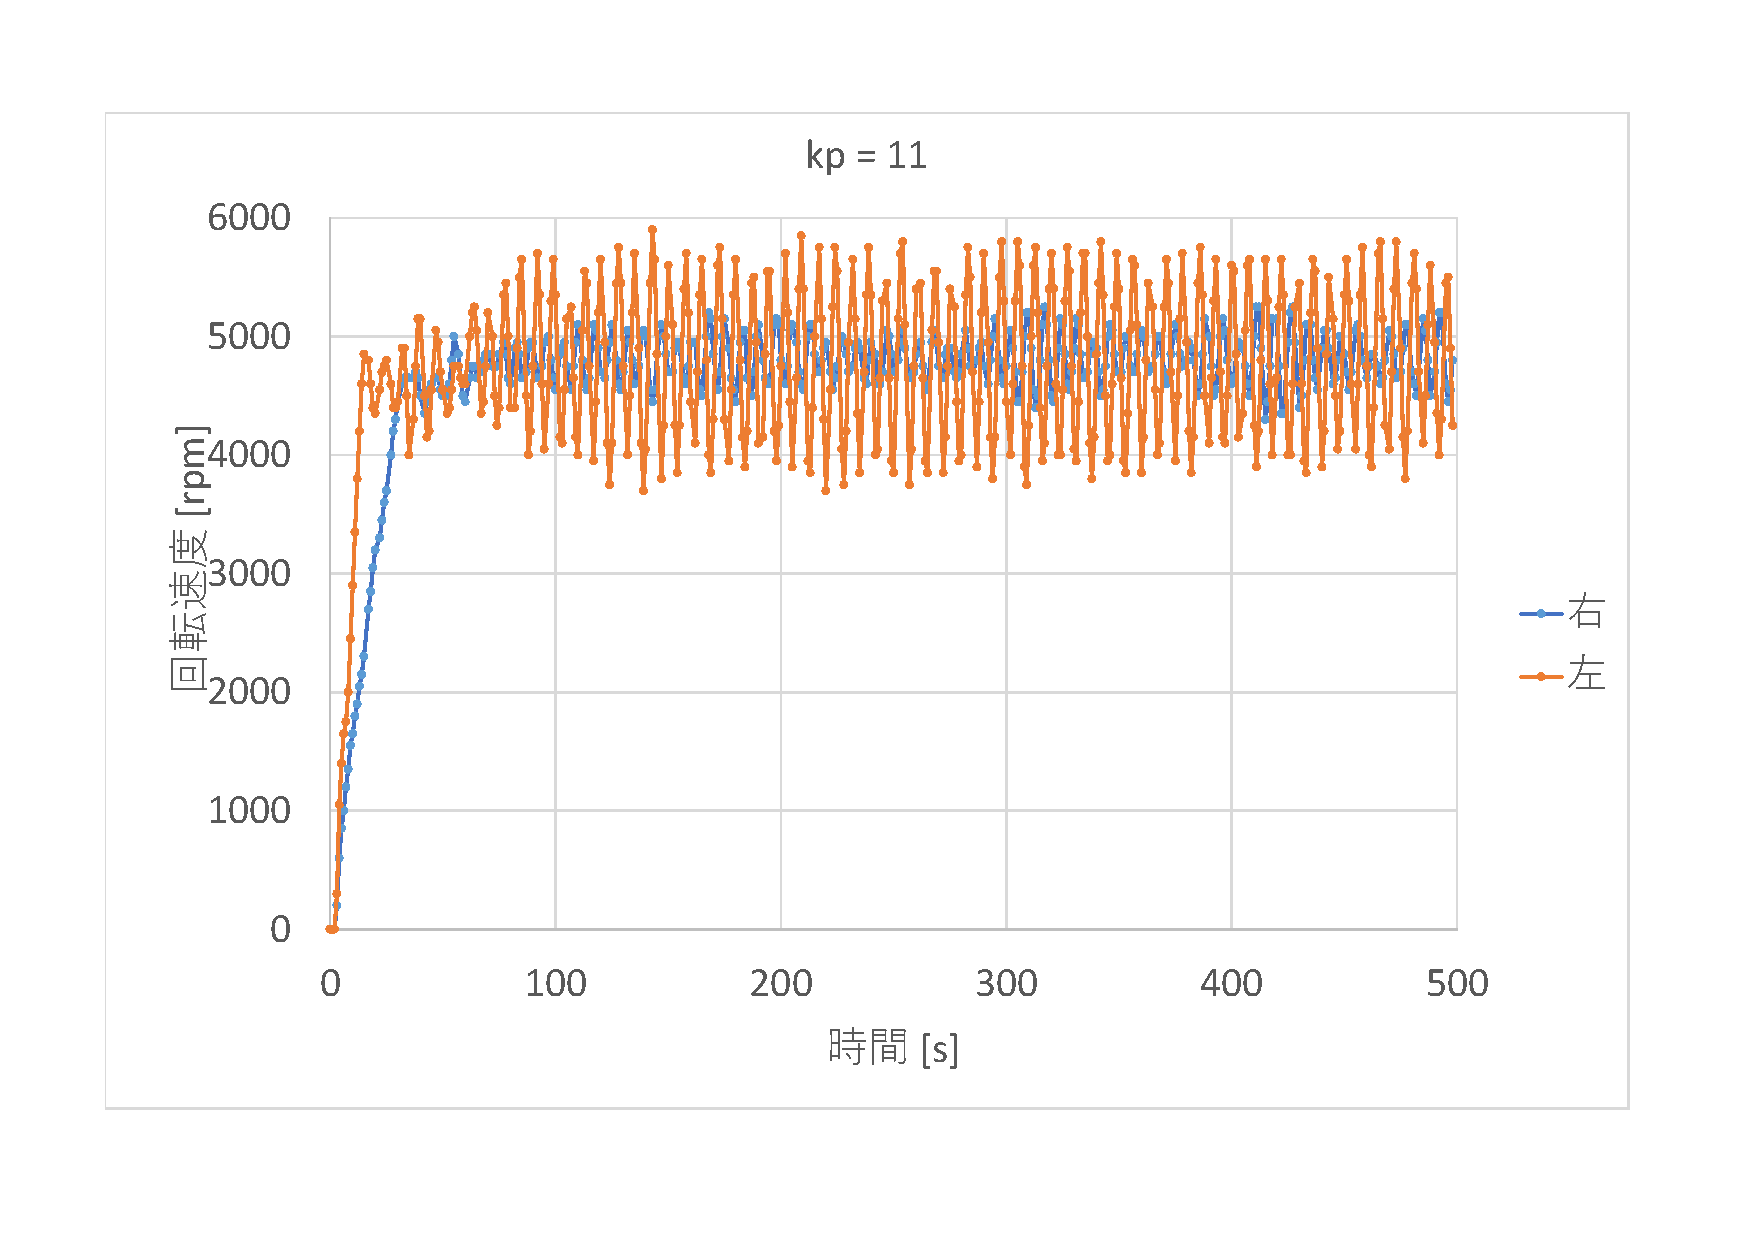
\includegraphics[width=\columnwidth]{img/13/DATA11.pdf}
  \label{im11}
  }
  \caption{ステップ応答のグラフ}
  \end{center}
\end{figure}

\begin{figure}[H]
  \begin{center}
  \subfigure[$k_p=12$]{
  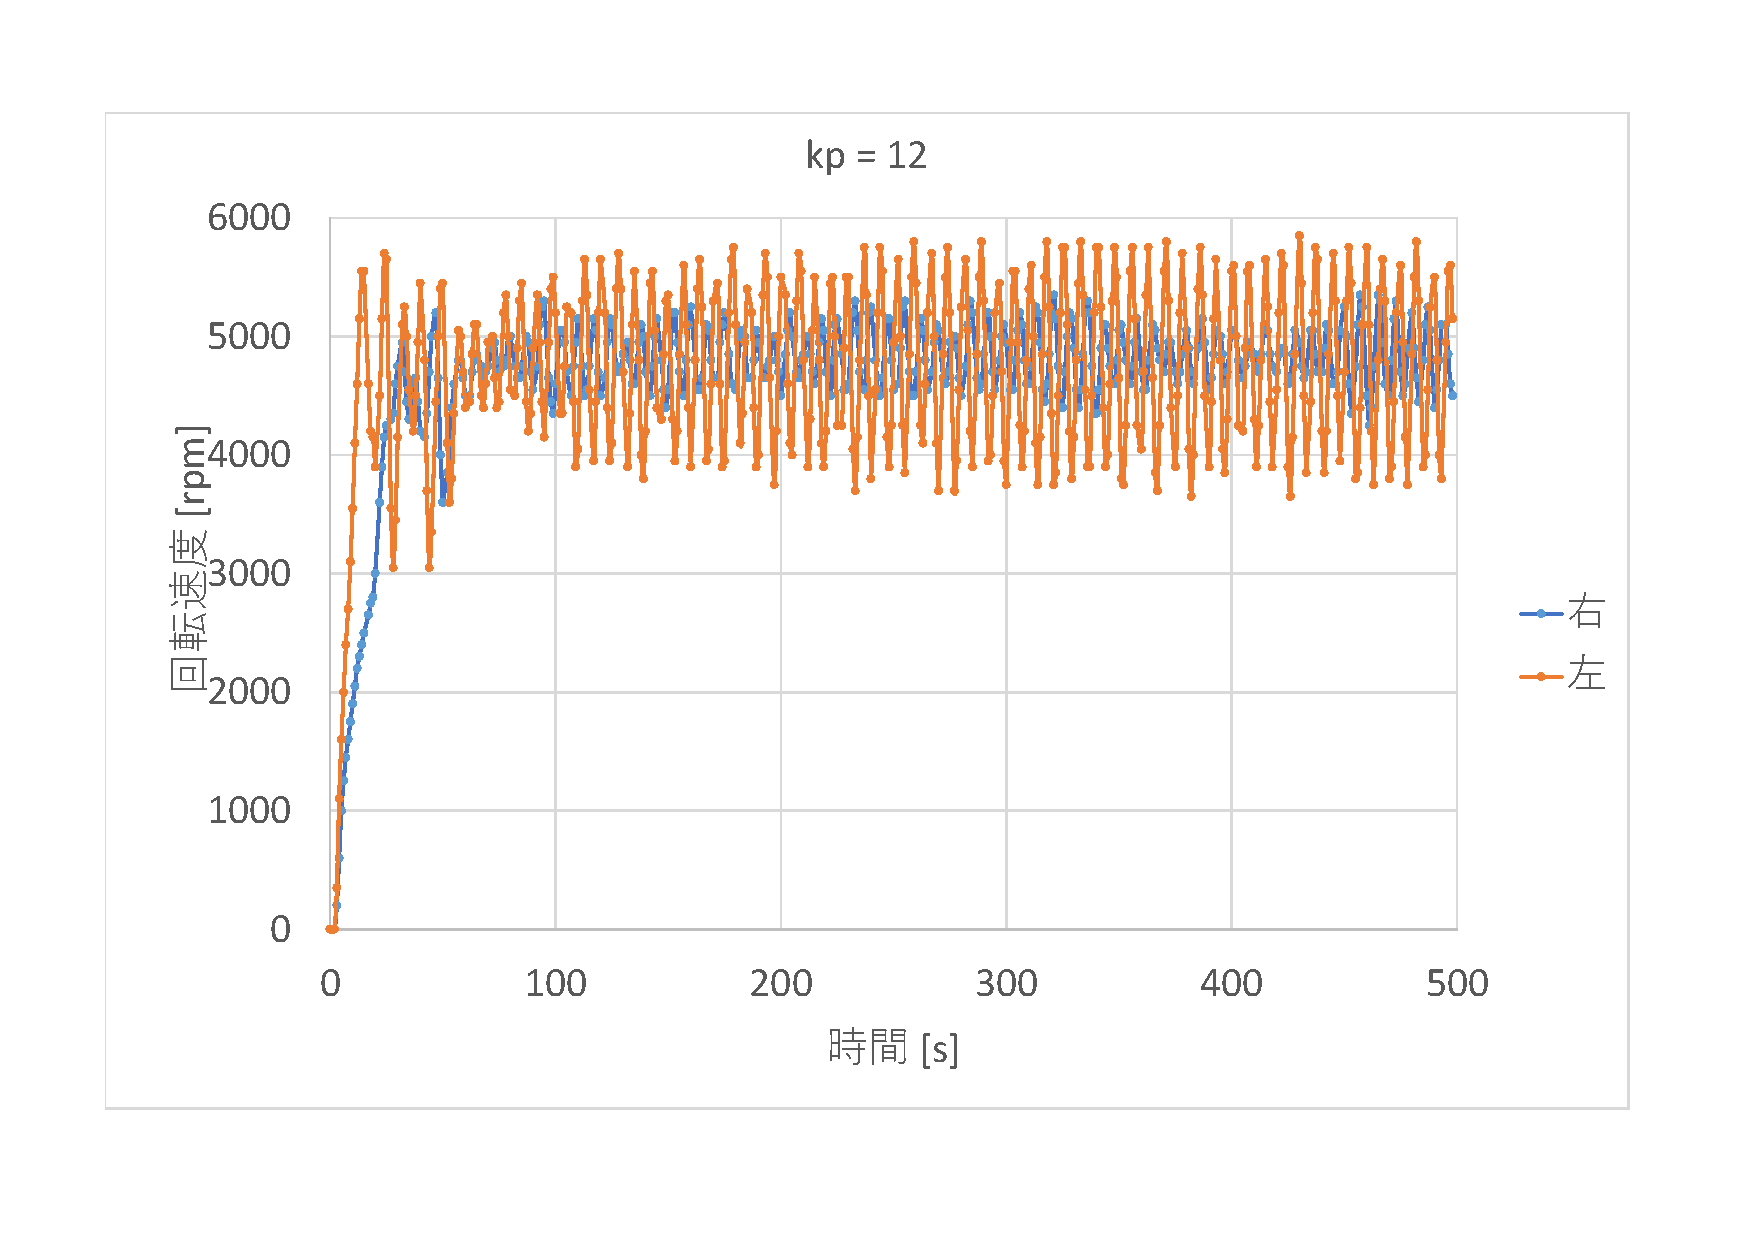
\includegraphics[width=\columnwidth]{img/13/DATA12.pdf}
  \label{im12}
  }
  \subfigure[$k_p=13$]{
  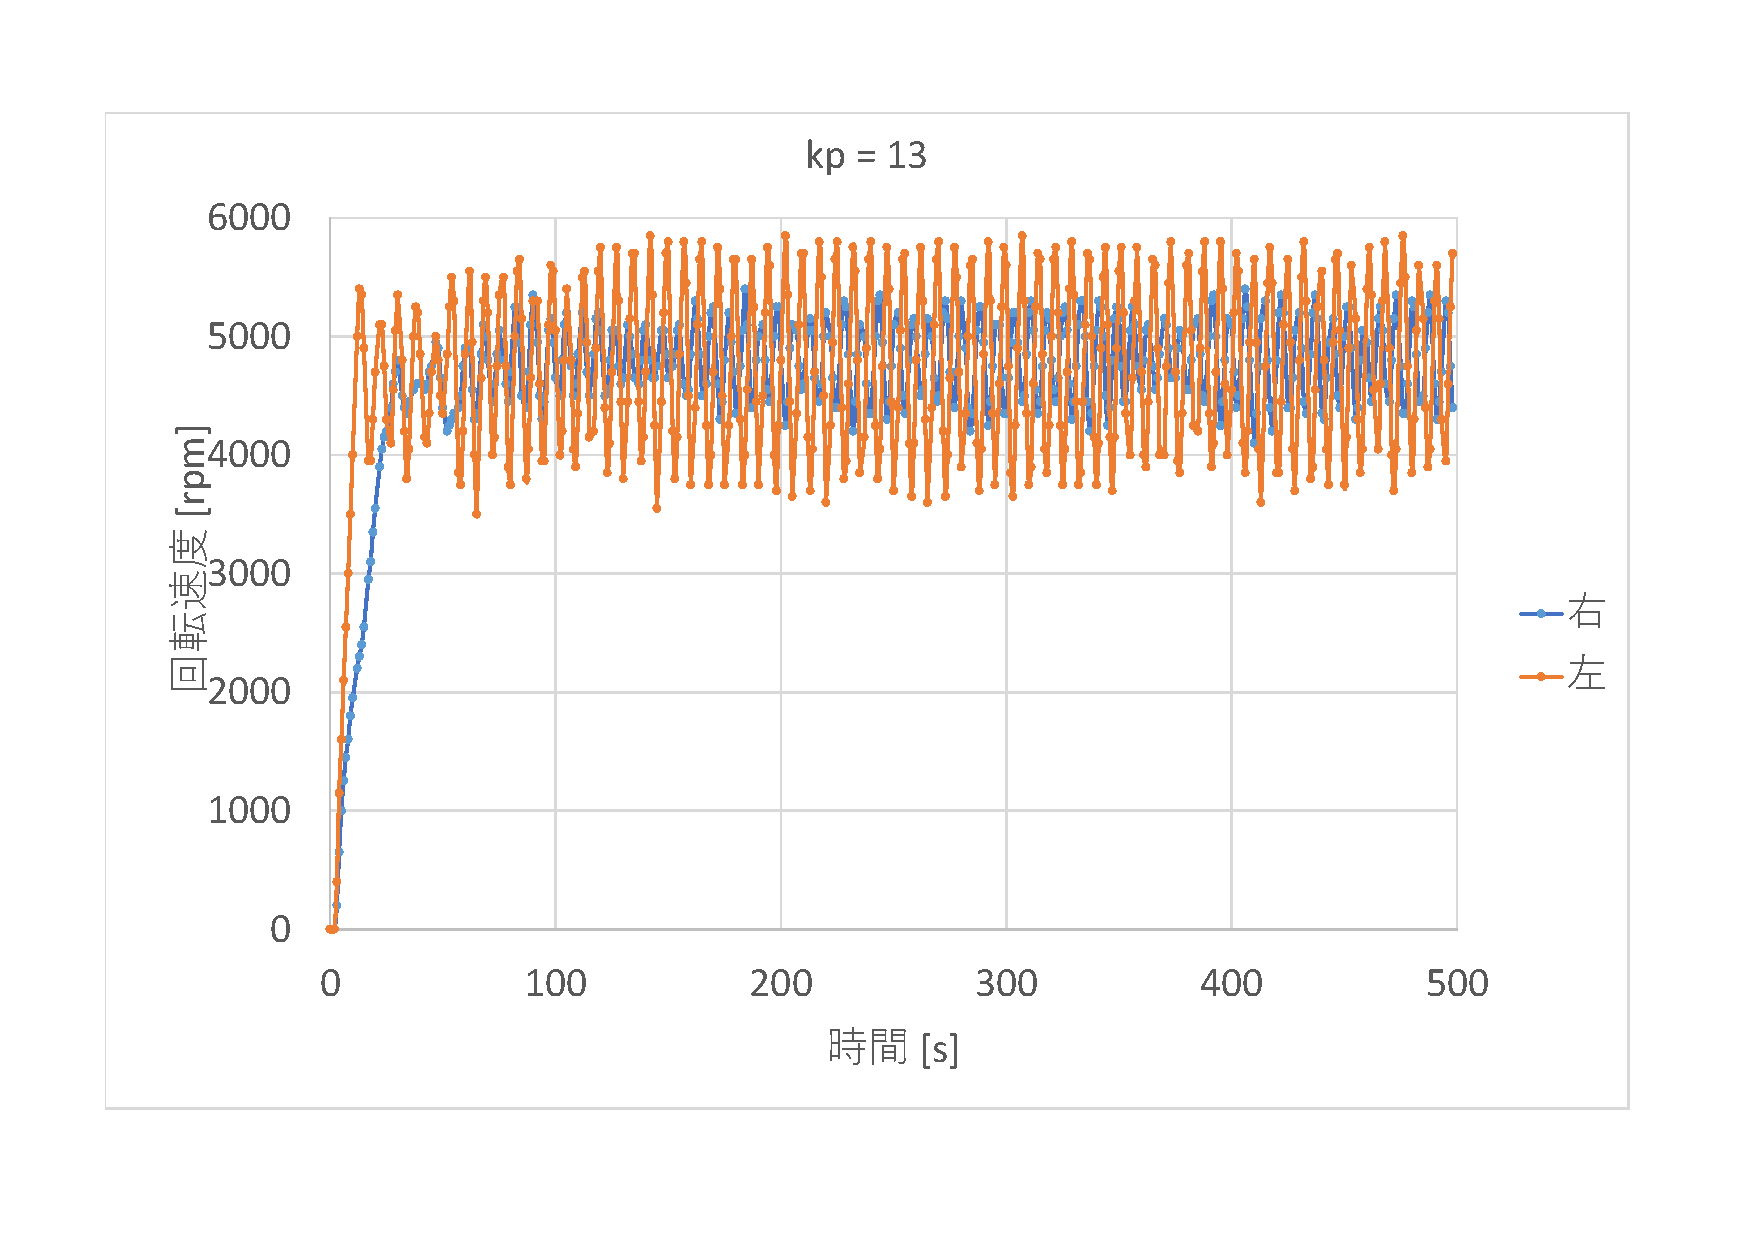
\includegraphics[width=\columnwidth]{img/13/DATA13.pdf}
  \label{im13}
  }
  \caption{ステップ応答のグラフ}
  \end{center}
\end{figure}
\begin{figure}[H]
  \begin{center}
  \subfigure[$k_p=14$]{
  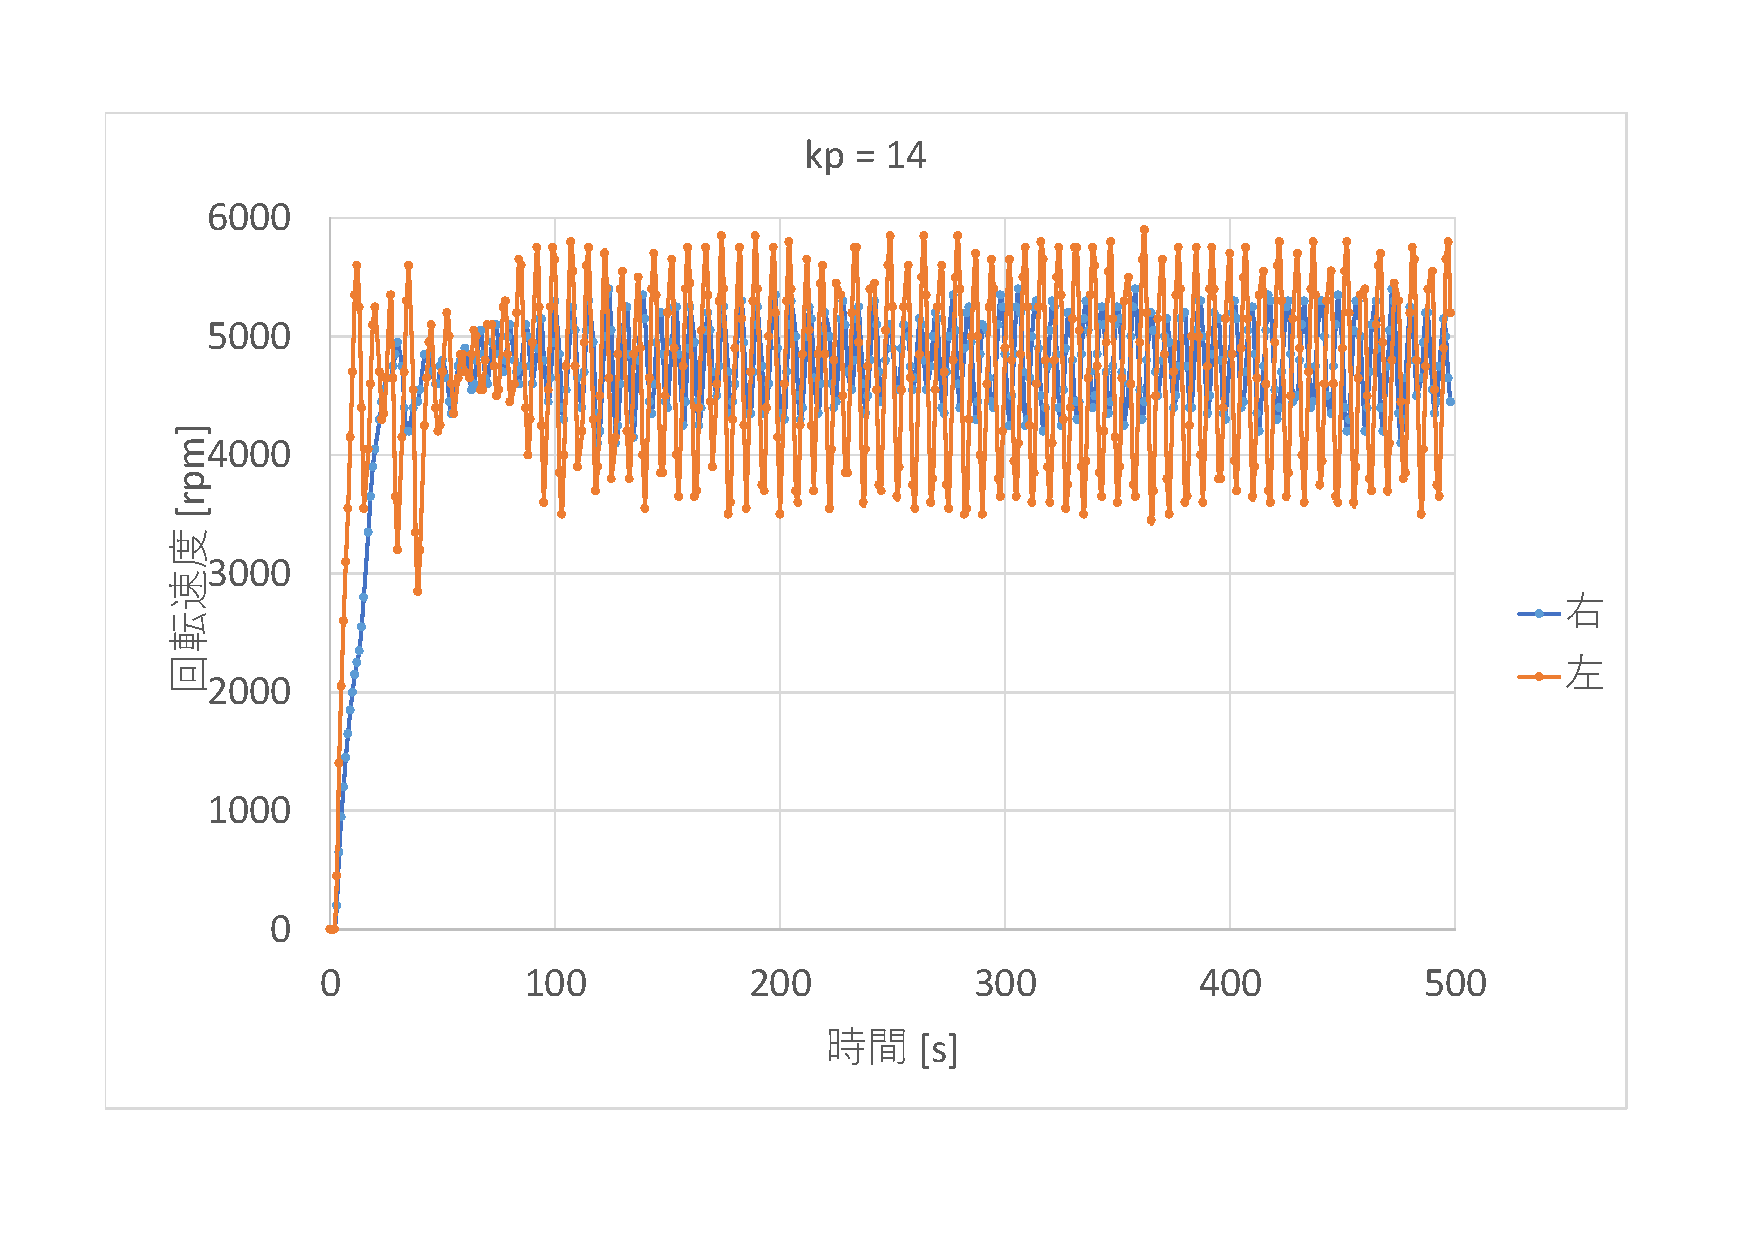
\includegraphics[width=\columnwidth]{img/13/DATA14.pdf}
  \label{im14}
  }
  \subfigure[$k_p=15$]{
  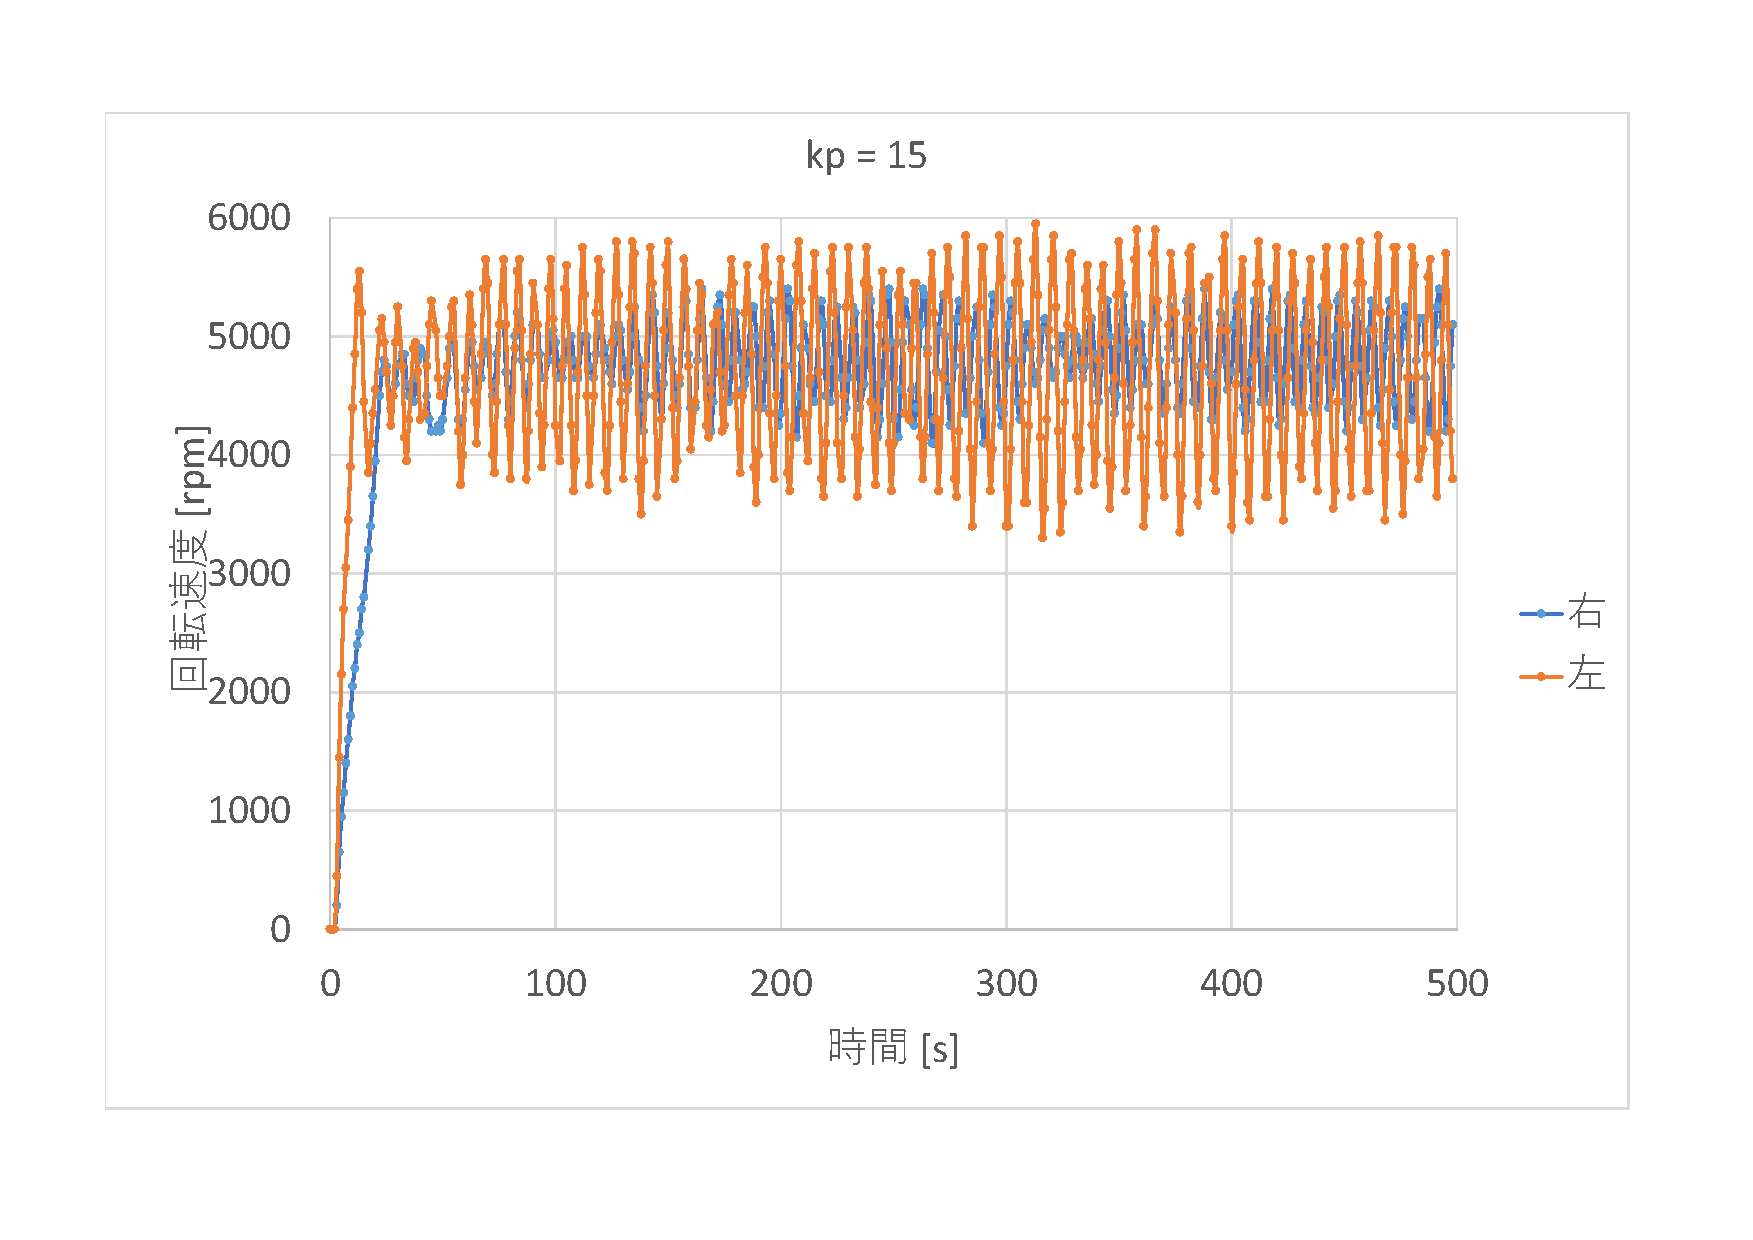
\includegraphics[width=\columnwidth]{img/13/DATA15.pdf}
  \label{im15}
  }
  \caption{ステップ応答のグラフ}
  \end{center}
\end{figure}

\section{演習14}
\subsection{実行プログラム}
実行プログラムをソースコード\ref{s14}に示す。
積分フィードバック係数\verb|ki_inv|$=$\verb|ms_read_dip()*1000|とした。

\begin{lstlisting}[caption=演習14のプログラム,label=s14]
#include <stdio.h>
#include <process.h>
#include <dos.h>
#include "v25.h"
#include "ms.h"
 
#define DMAX 500
  
int main(){
    int i;
    int kp, ki_inv;
    int vrefl, vrefr;
    int vl[DMAX], vr[DMAX];
    long ct, ctm, t[DMAX];
    FILE *fp;
  
    ms_init();
  
    kp = 7;
    ki_inv = ms_read_dip()*1000;
    vrefl = 5000;
    vrefr = 5000;
  
    ms_motor_on();
    ms_read_v(&vl[0], &vr[0], &ctm);
    ms_step_res(vrefl, vrefr, kp, ki_inv);
  for(i=1; i<DMAX; i++){
    ms_read_v(&vl[i], &vr[i], &ct);
    t[i] = ct - ctm;
    ms_wait(2);
  }
  ms_motor_off();
  
  if((fp = fopen("data.dat", "wt")) == NULL){
    printf("Can't Open File!!\n");
    exit(1);
  }
  
  for(i=1; i<DMAX; i++){
    fprintf(fp, "%7d %7d %10ld\n", vl[i], vr[i], t[i]);
  }
  fclose(fp);
  ms_beep(440,500);
  printf("owari\n");
  return 0;
}
\end{lstlisting}

\subsection{実行結果}
演習13と同様に
モータのステップ応答(回転速度と時間)
をデータファイルに保存する。
応答グラフを図\ref{im15_14}\verb|~|\ref{im1_14}に示す。
積分フィードバック係数$k_i=1/13000$を最適な値とした。
つまり、\verb|ms_read_dip()|$=$\tsuyo{13}の値である。

\begin{figure}[H]
  \begin{center}
  \subfigure[$k_i=1/15000$]{
  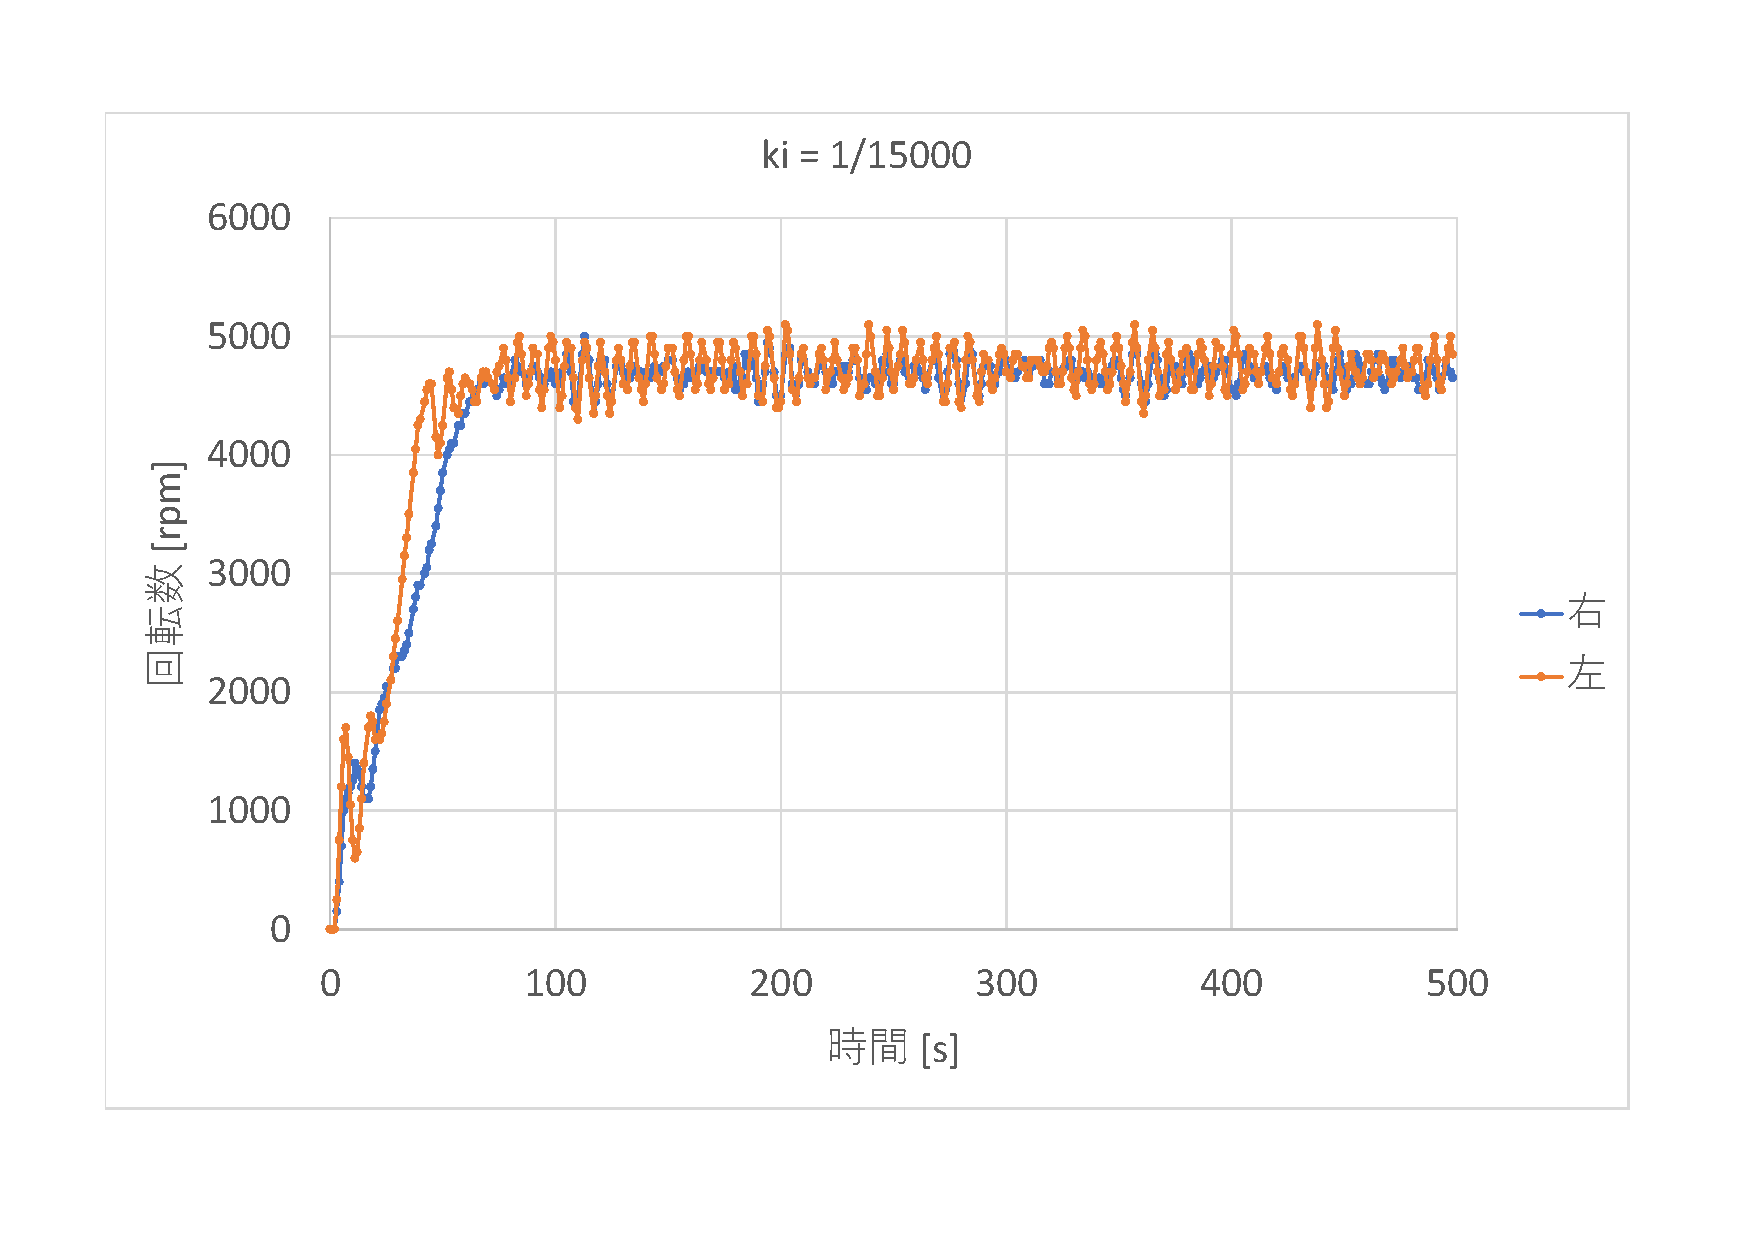
\includegraphics[width=.7\columnwidth]{img/14/DATA15.pdf}
  \label{im15_14}
  }
  \subfigure[$k_i=1/14000$]{
  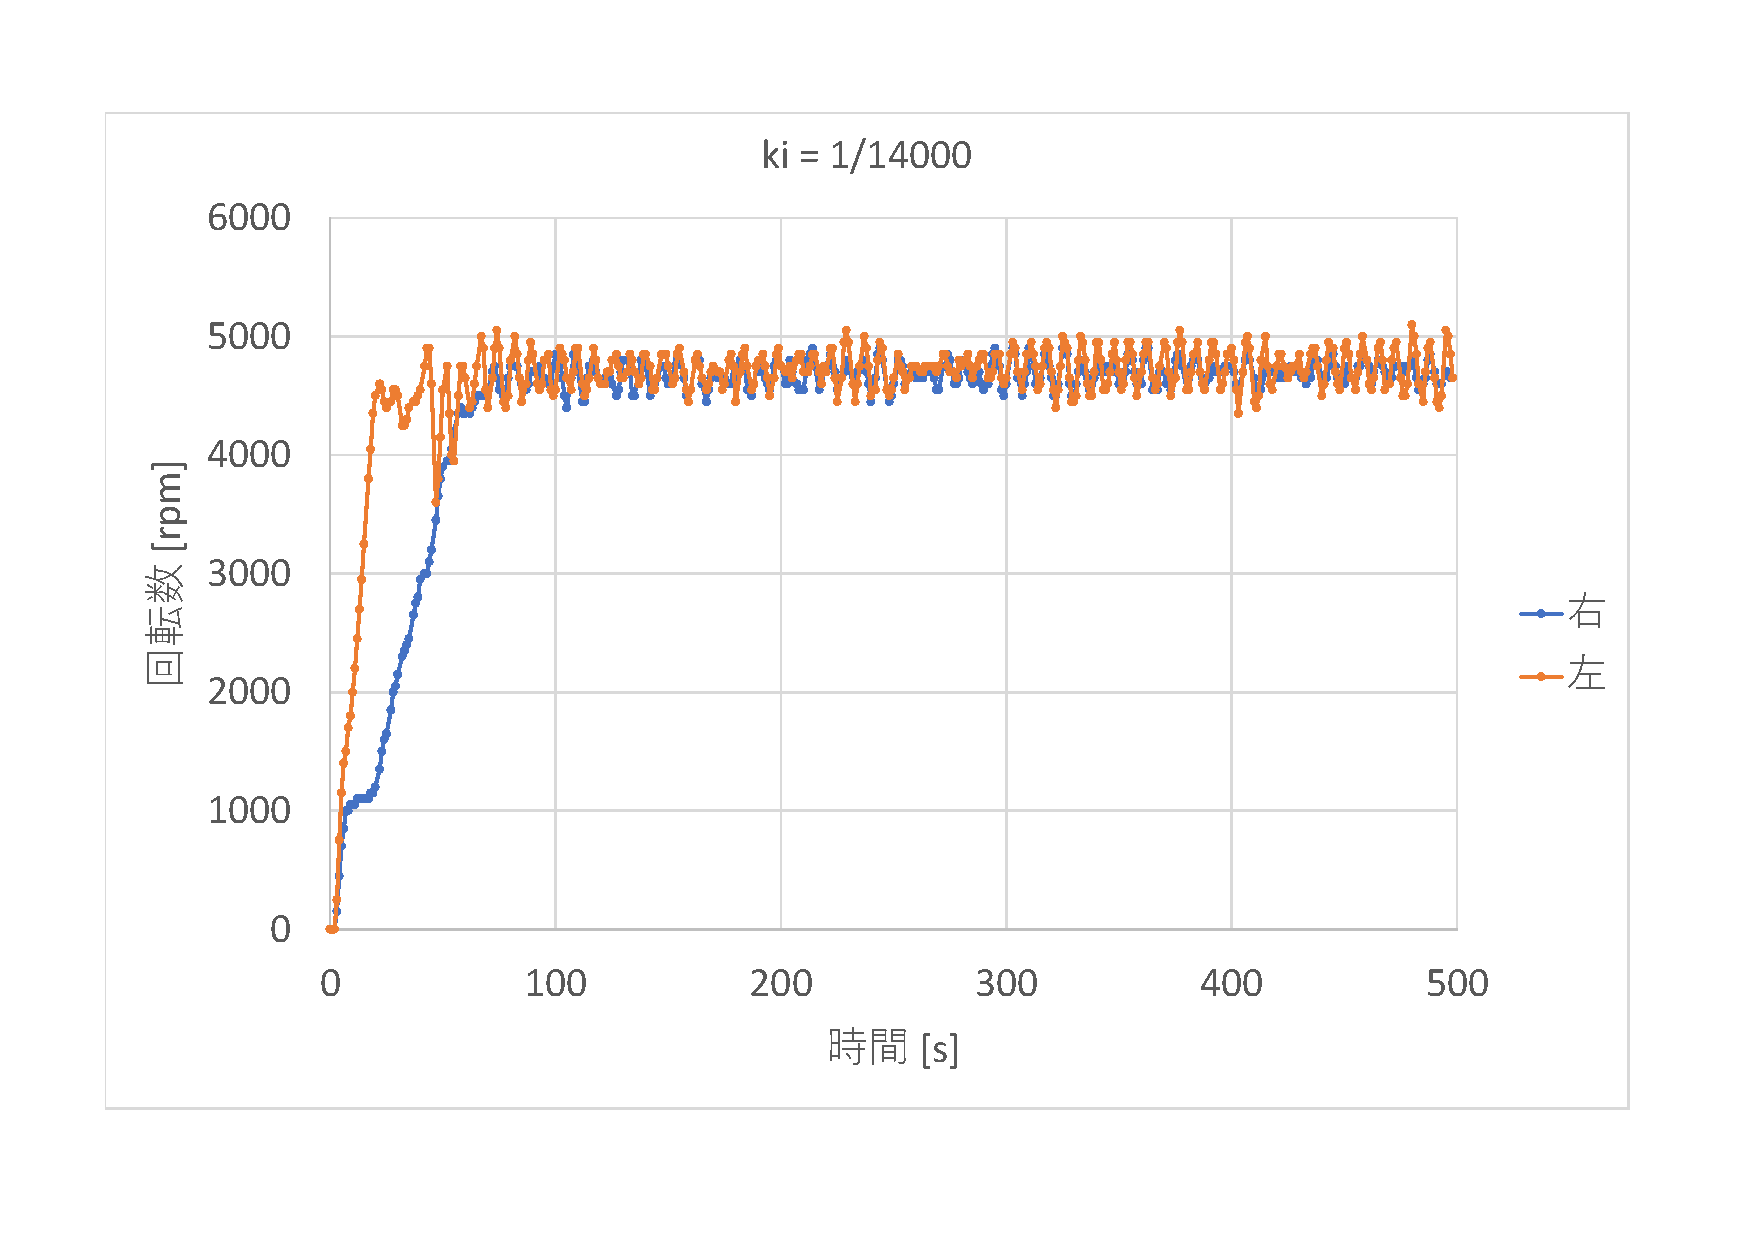
\includegraphics[width=.7\columnwidth]{img/14/DATA14.pdf}
  \label{im14_14}
  }
  \caption{ステップ応答のグラフ}
  \end{center}
\end{figure}
\begin{figure}[H]
  \begin{center}
  \subfigure[$k_i=1/13000$]{
  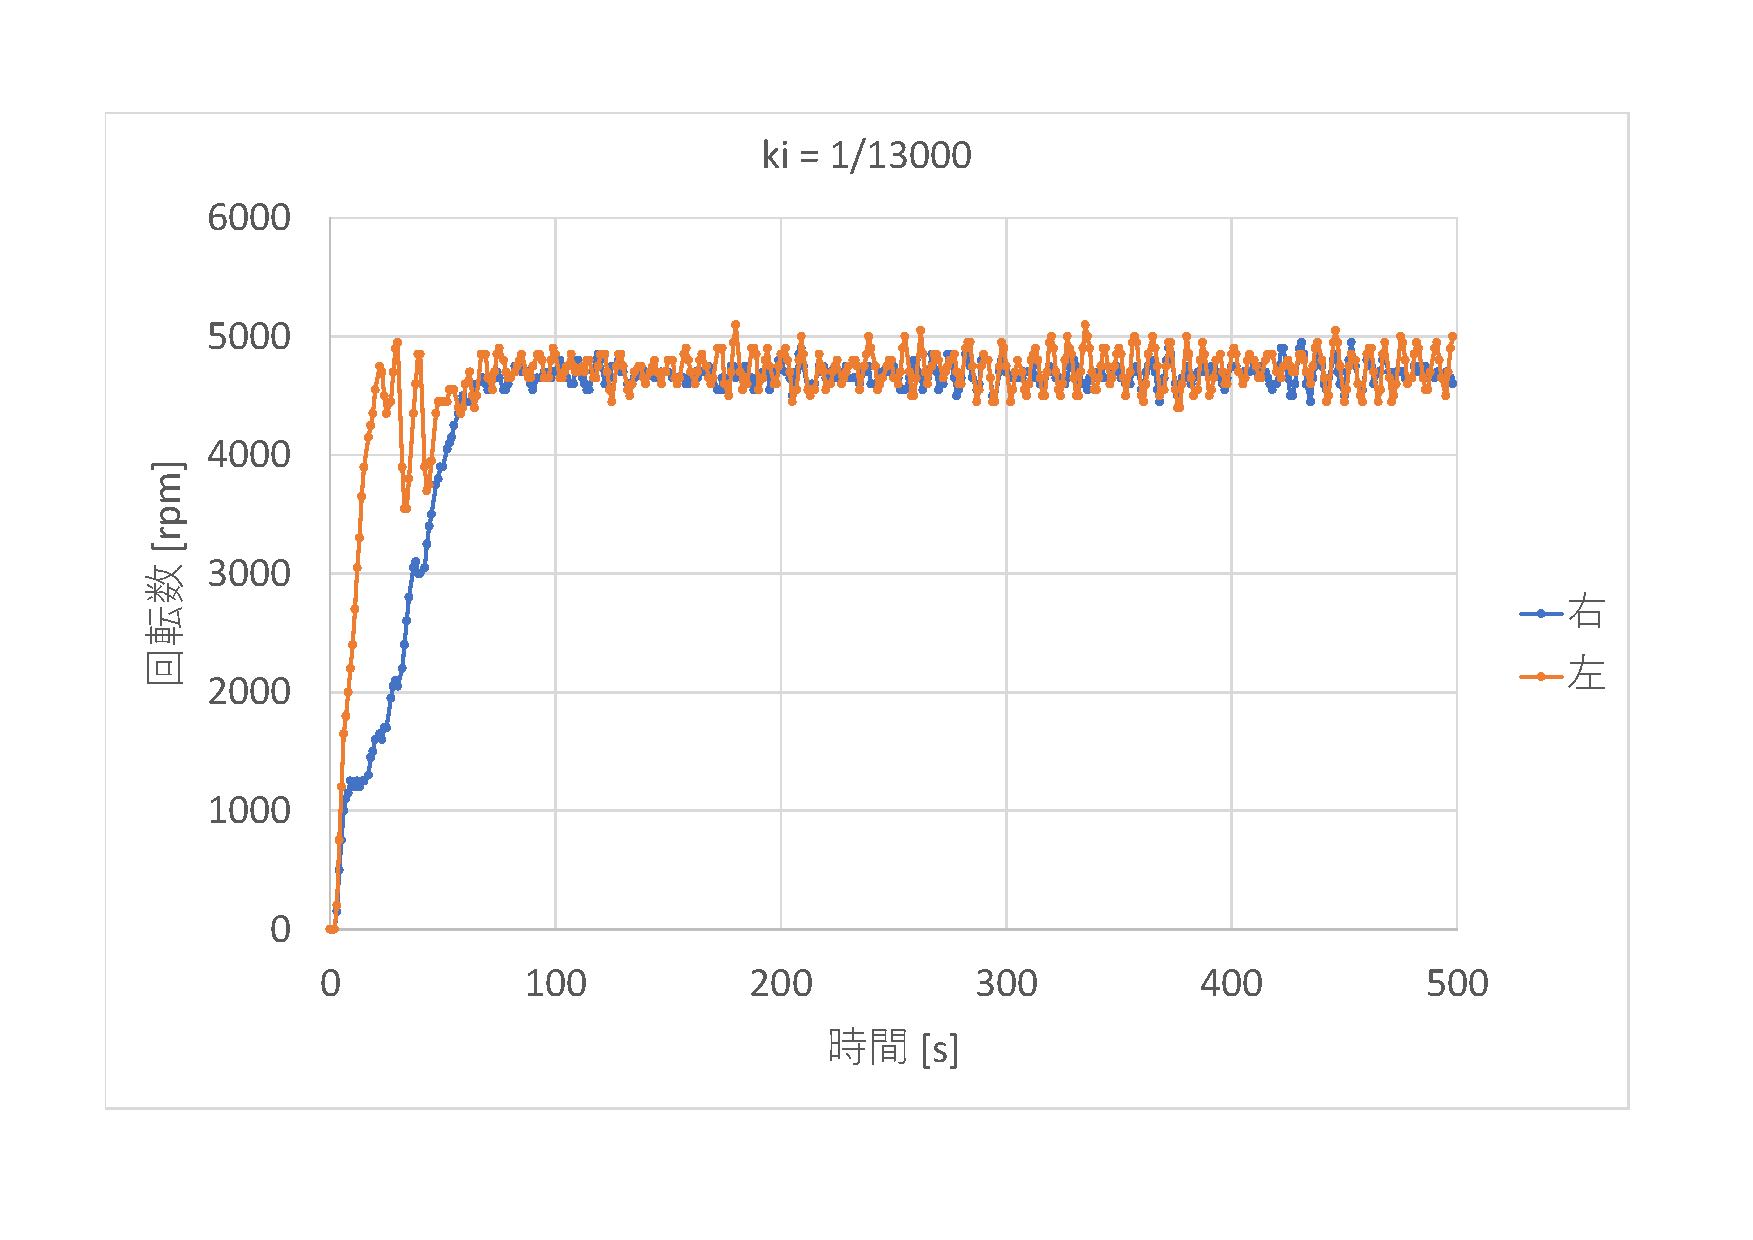
\includegraphics[width=\columnwidth]{img/14/DATA13.pdf}
  \label{im13_14}
  }
  \subfigure[$k_i=1/12000$]{
  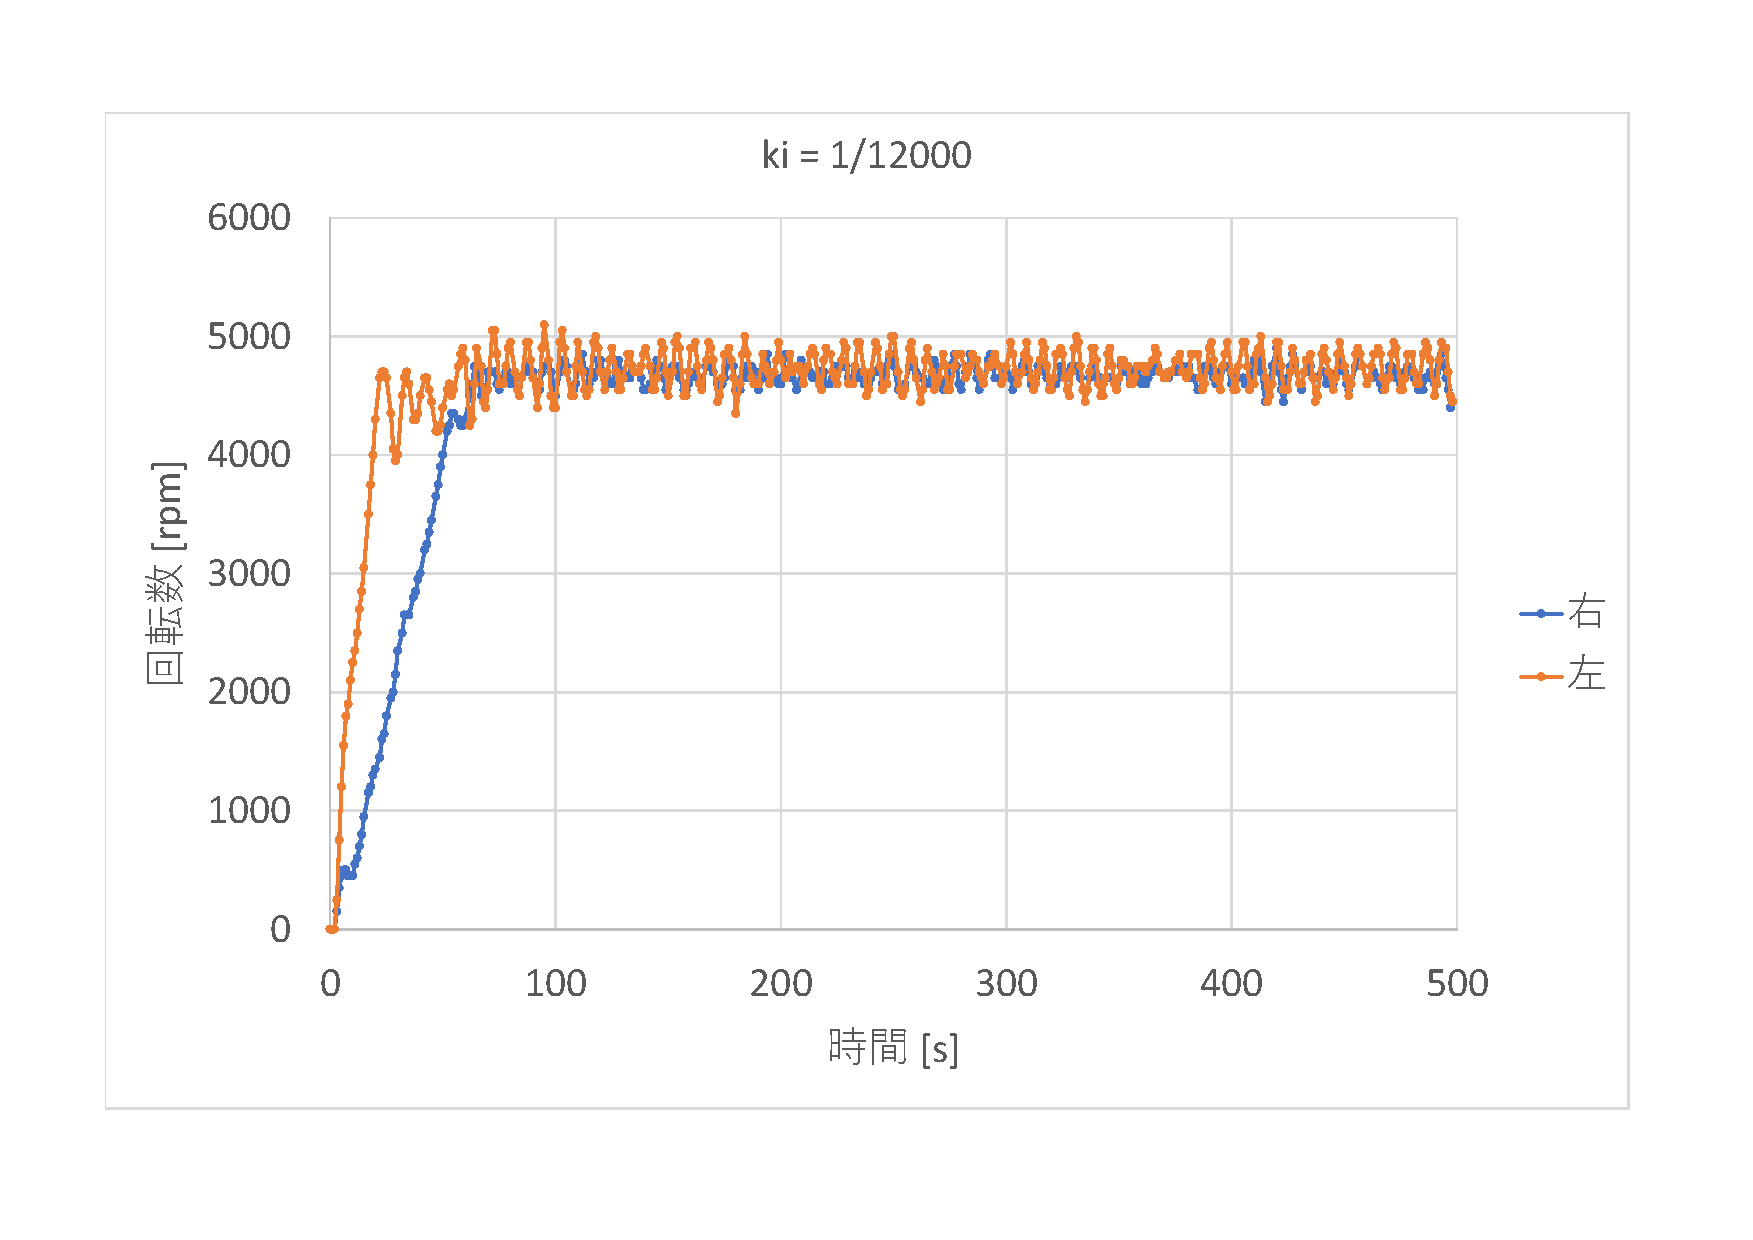
\includegraphics[width=\columnwidth]{img/14/DATA12.pdf}
  \label{im12_14}
  }
  \caption{ステップ応答のグラフ}
  \end{center}
\end{figure}
\begin{figure}[H]
  \begin{center}
  \subfigure[$k_i=1/11000$]{
  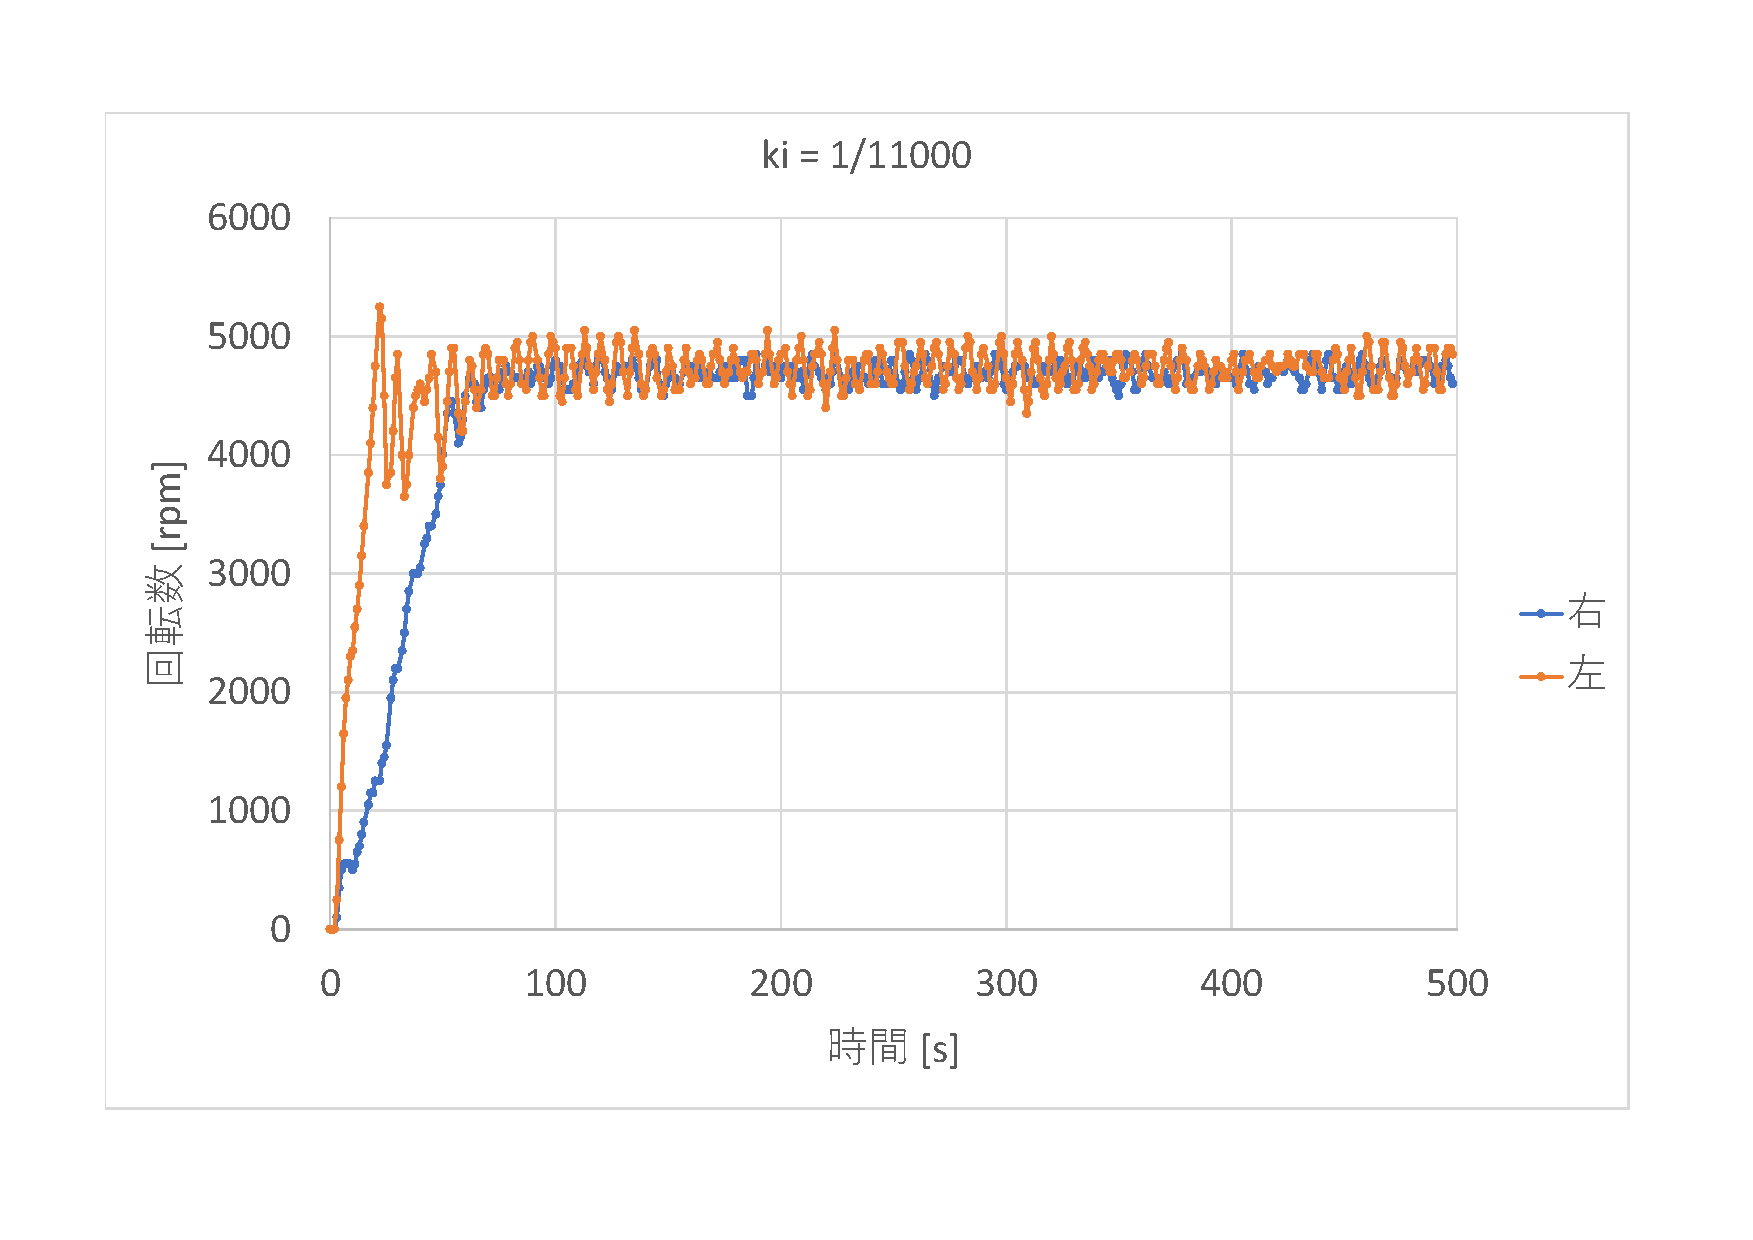
\includegraphics[width=\columnwidth]{img/14/DATA11.pdf}
  \label{im11_14}
  }
  \subfigure[$k_i=1/10000$]{
  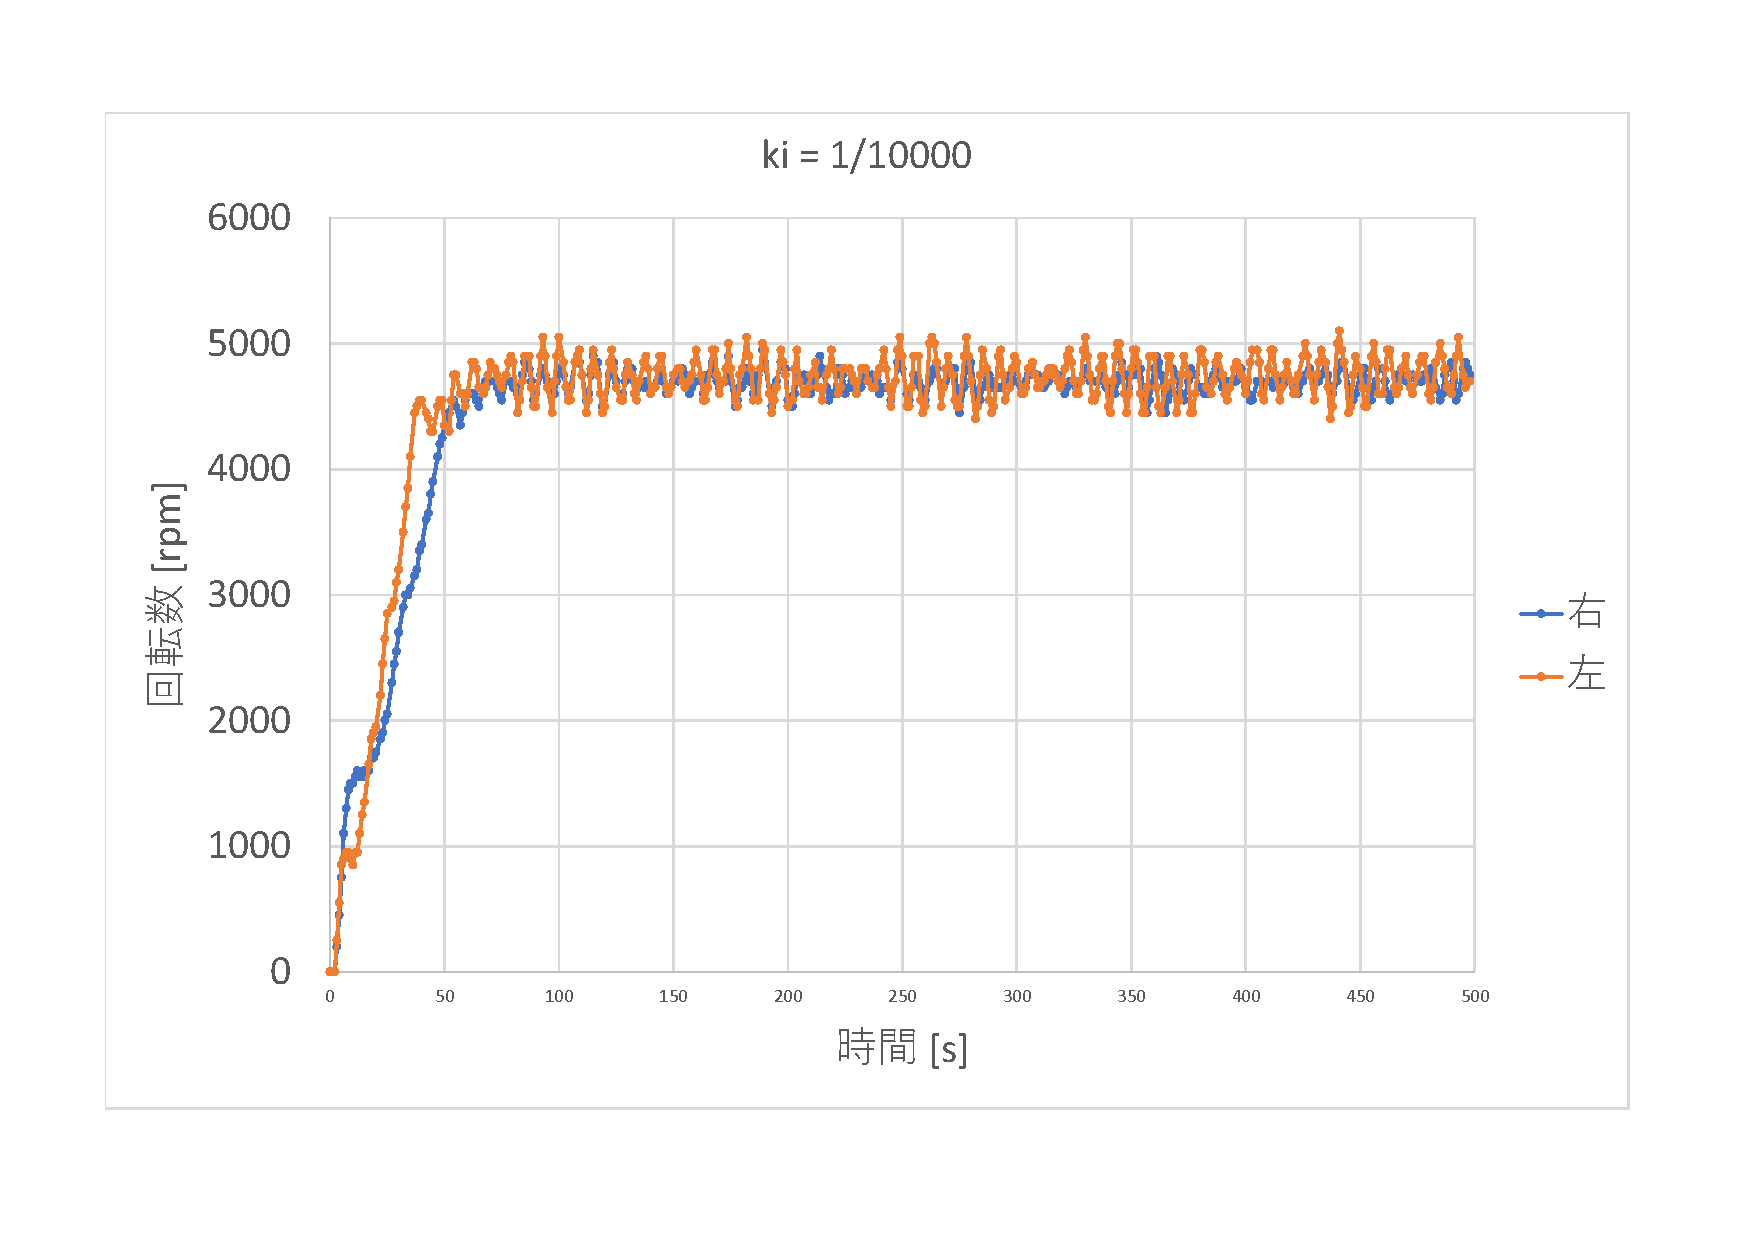
\includegraphics[width=\columnwidth]{img/14/DATA10.pdf}
  \label{im10_14}
  }
  \caption{ステップ応答のグラフ}
  \end{center}
\end{figure}
\begin{figure}[H]
  \begin{center}
  \subfigure[$k_i=1/9000$]{
  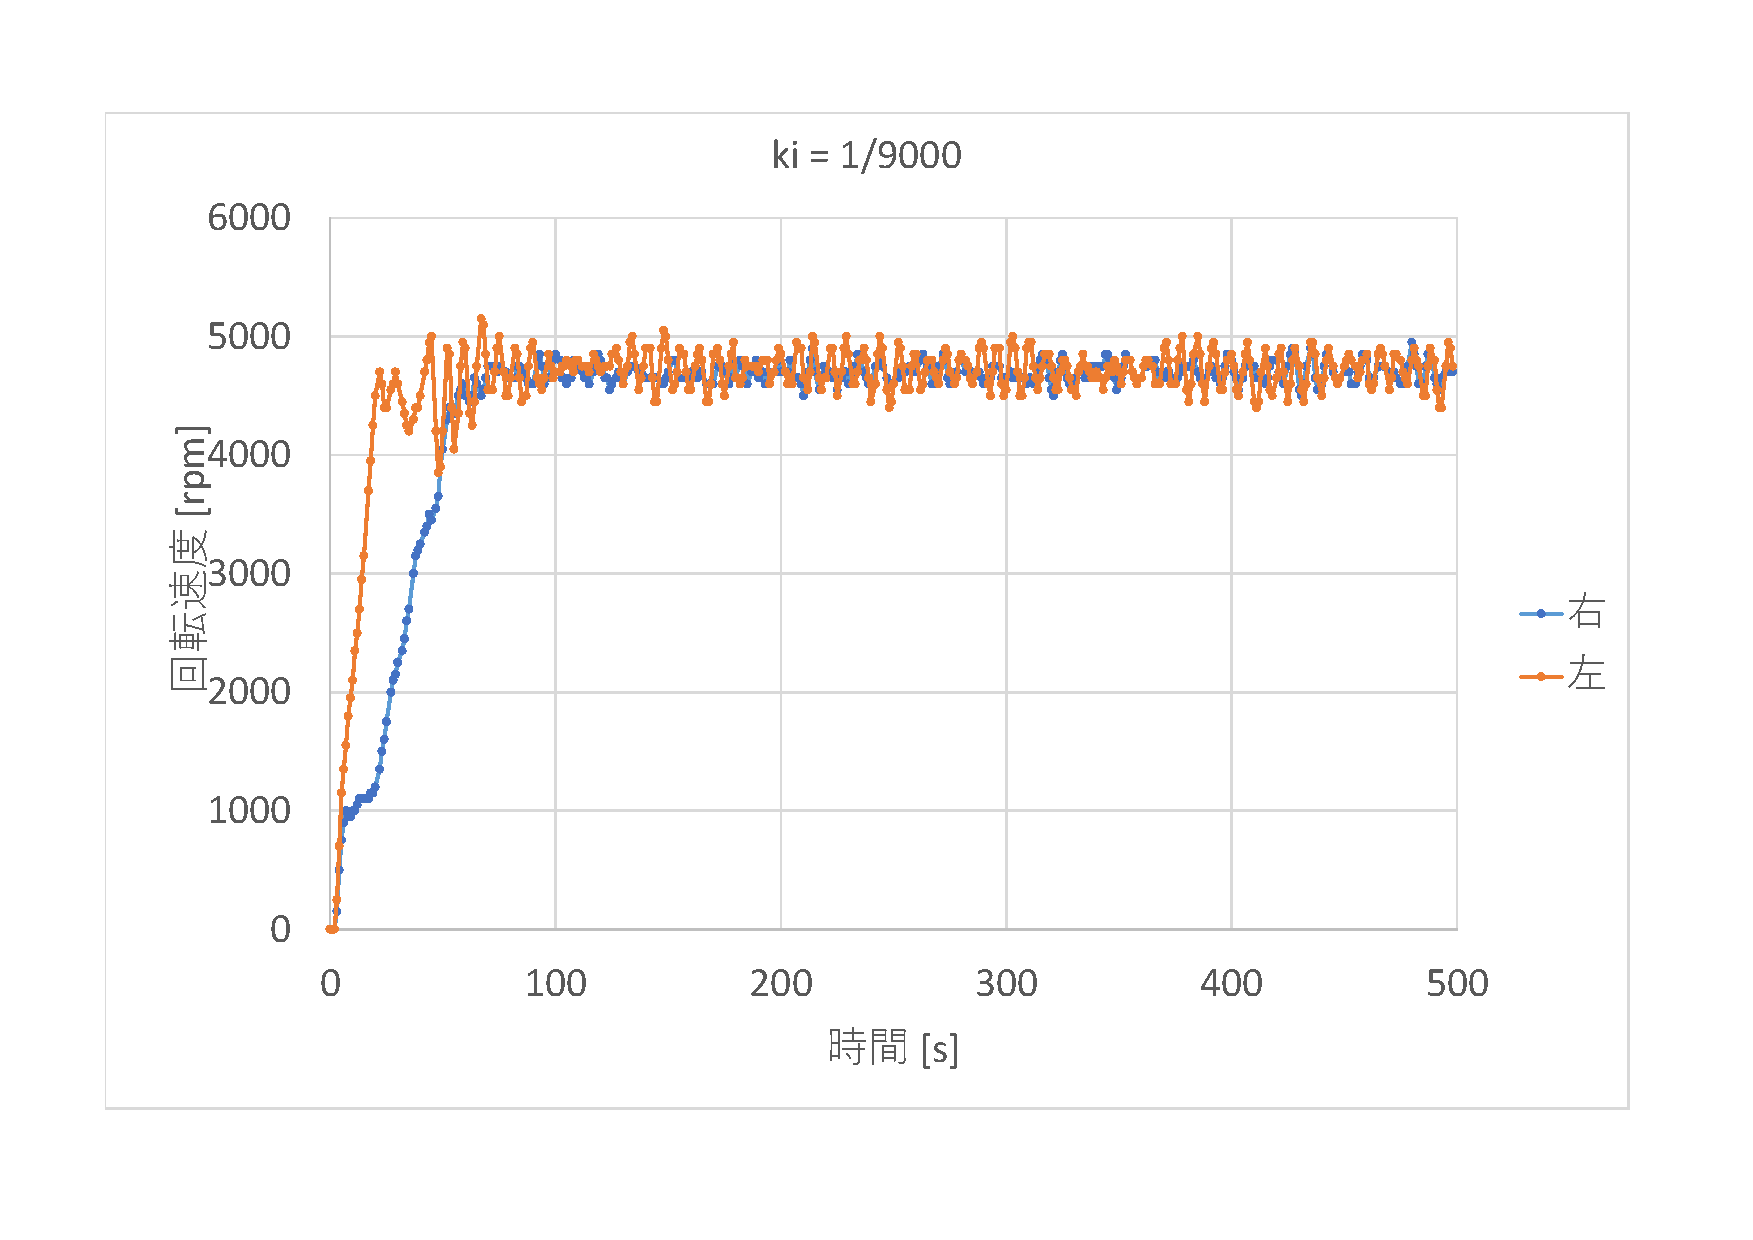
\includegraphics[width=\columnwidth]{img/14/DATA9.pdf}
  \label{im9_14}
  }
  \subfigure[$k_i=1/8000$]{
  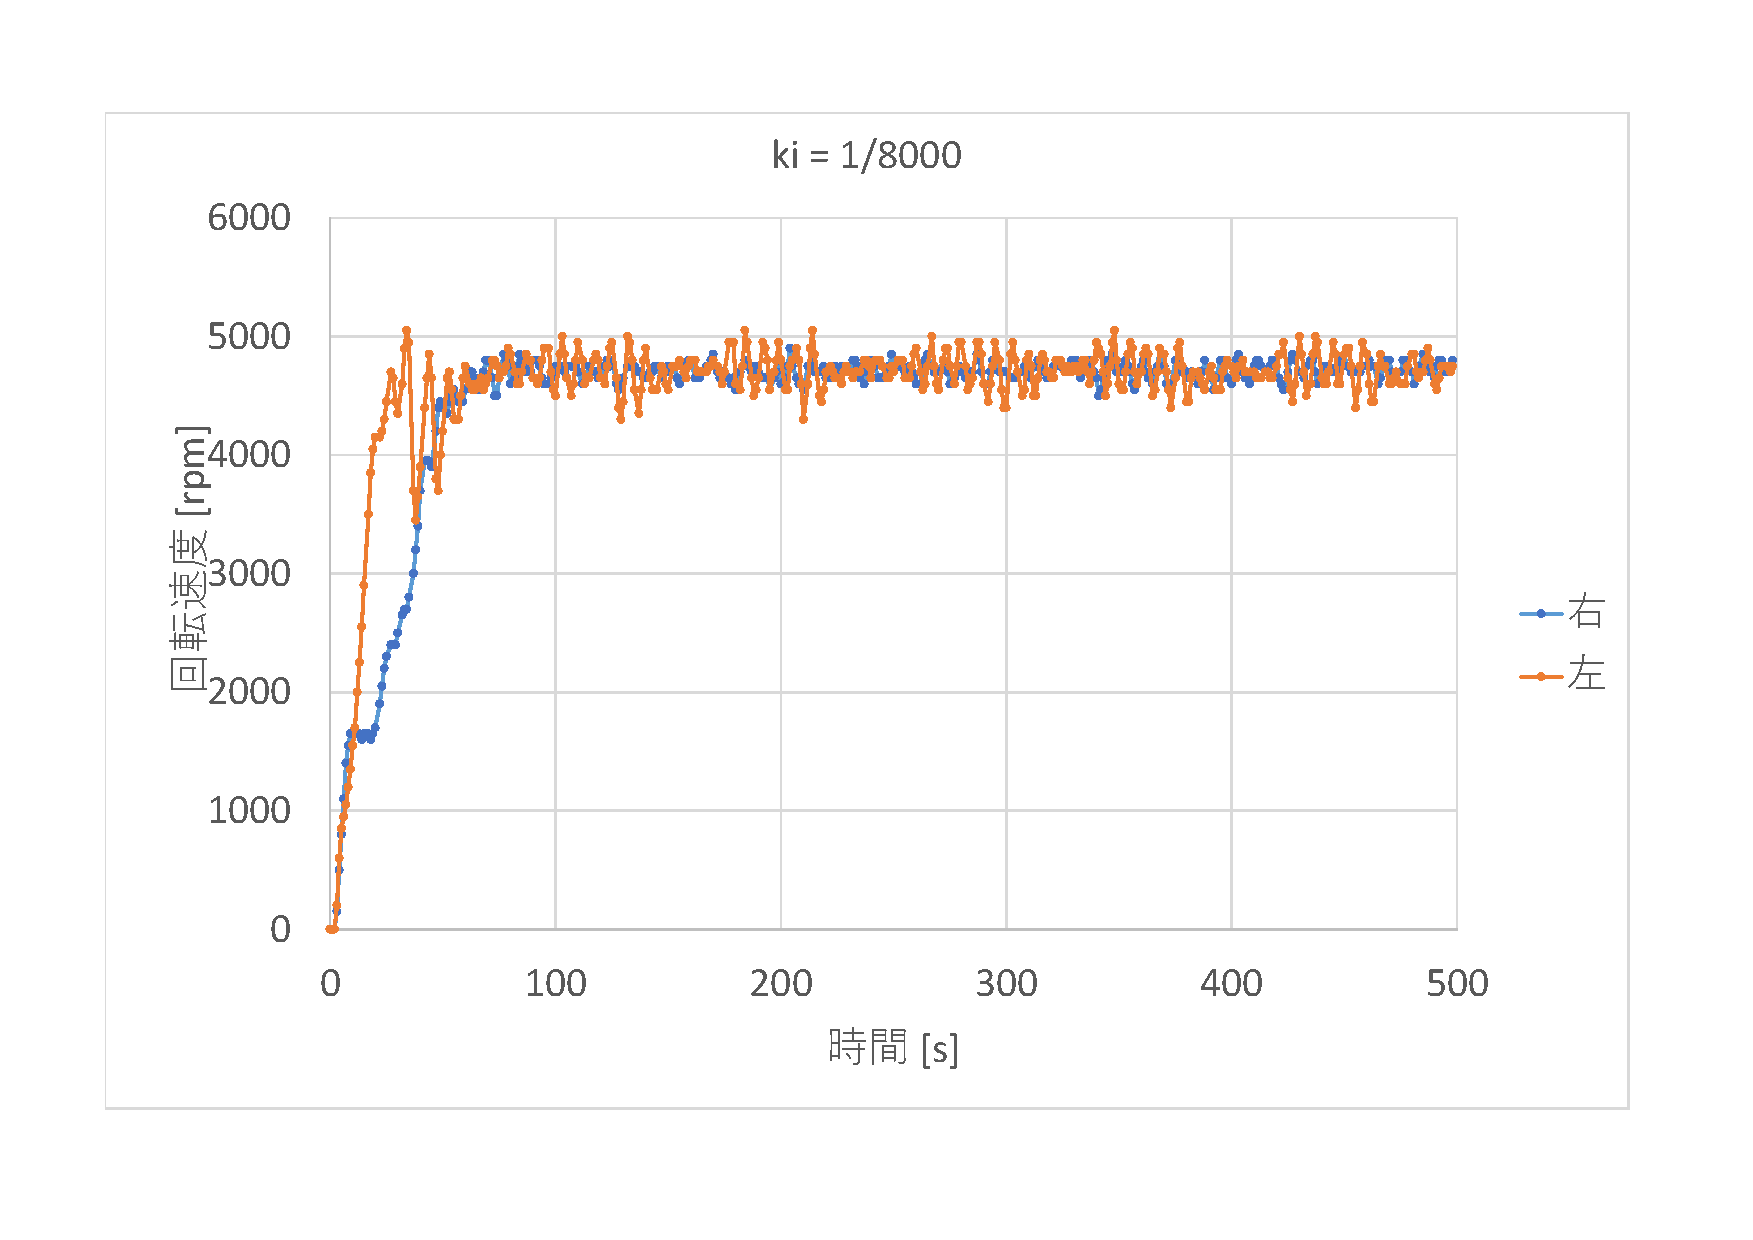
\includegraphics[width=\columnwidth]{img/14/DATA8.pdf}
  \label{im8_14}
  }
  \end{center}
\end{figure}
\begin{figure}[H]
  \begin{center}
  \subfigure[$k_i=1/7000$]{
  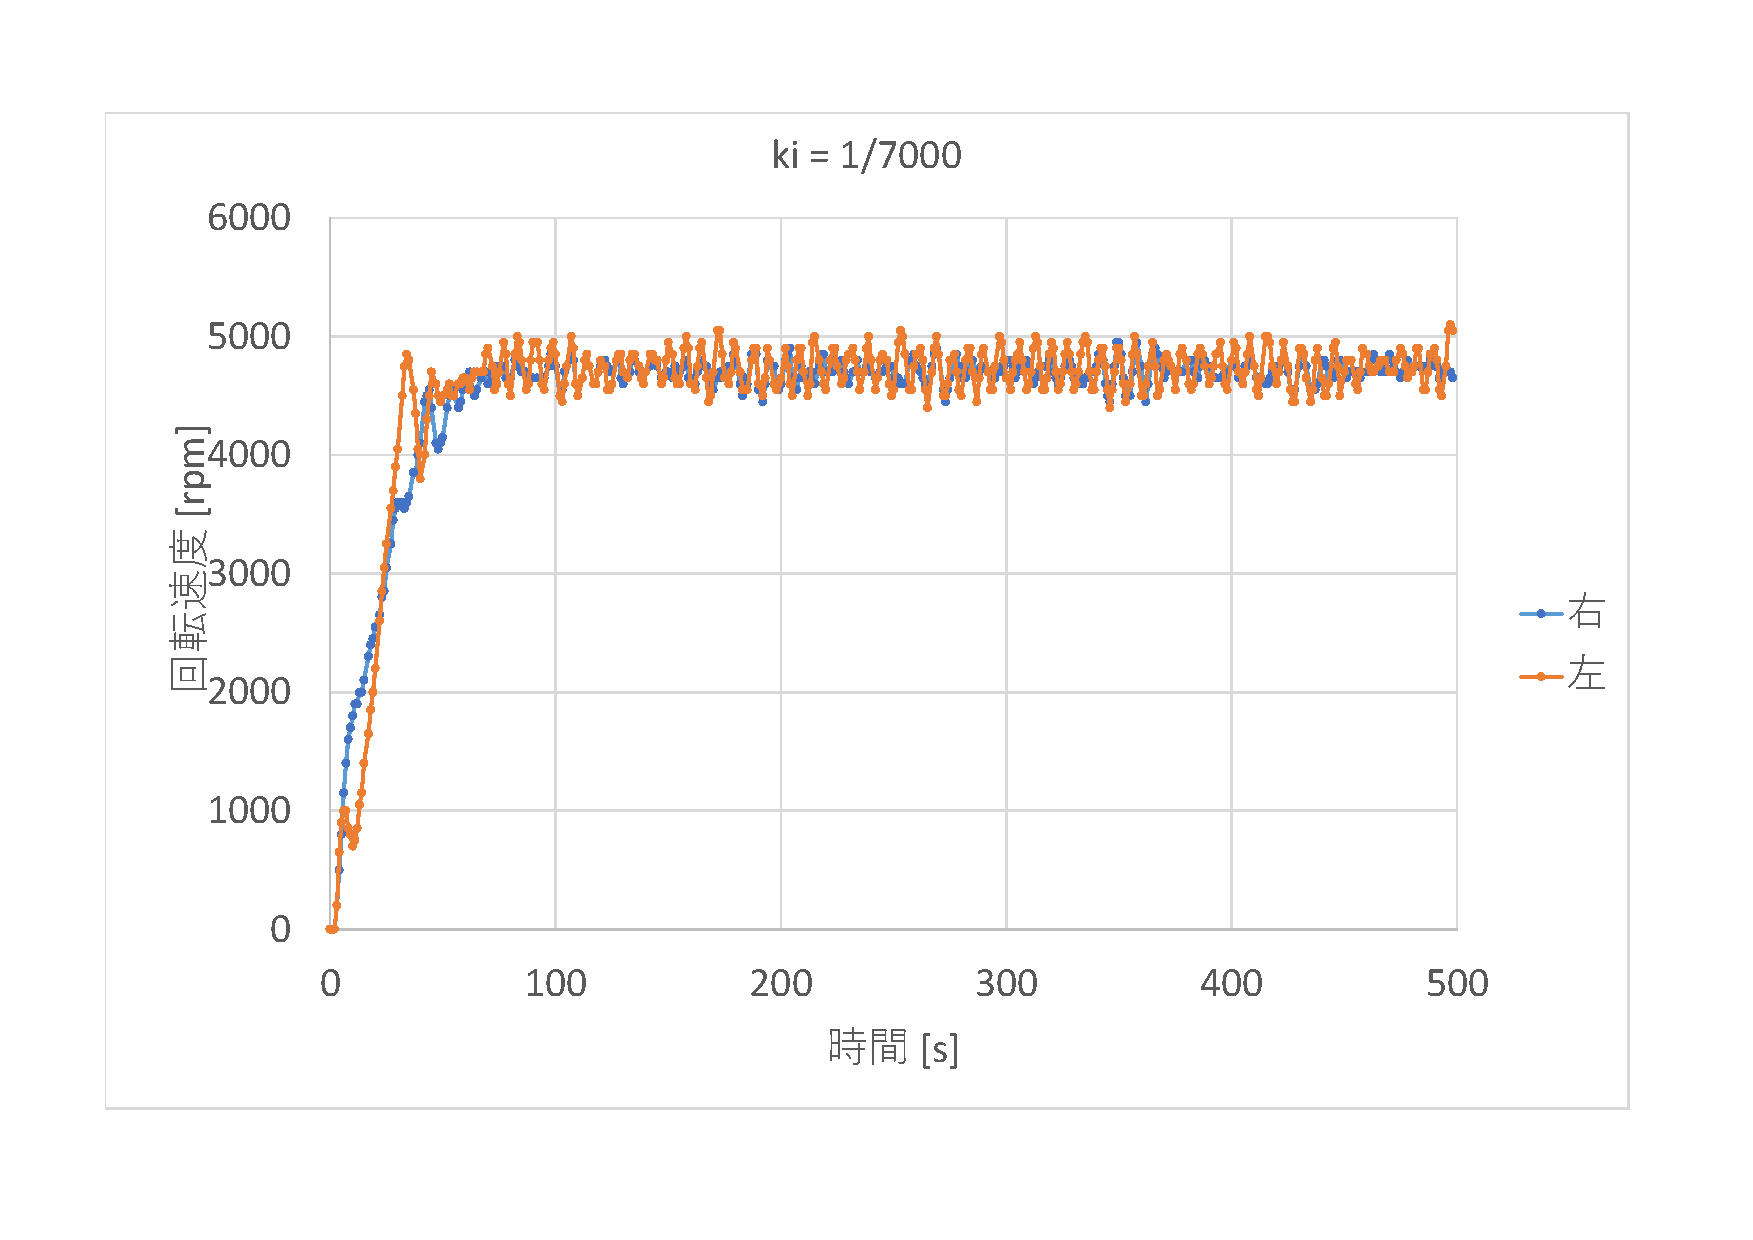
\includegraphics[width=\columnwidth]{img/14/DATA7.pdf}
  \label{im7_14}
  }
  \subfigure[$k_i=1/6000$]{
  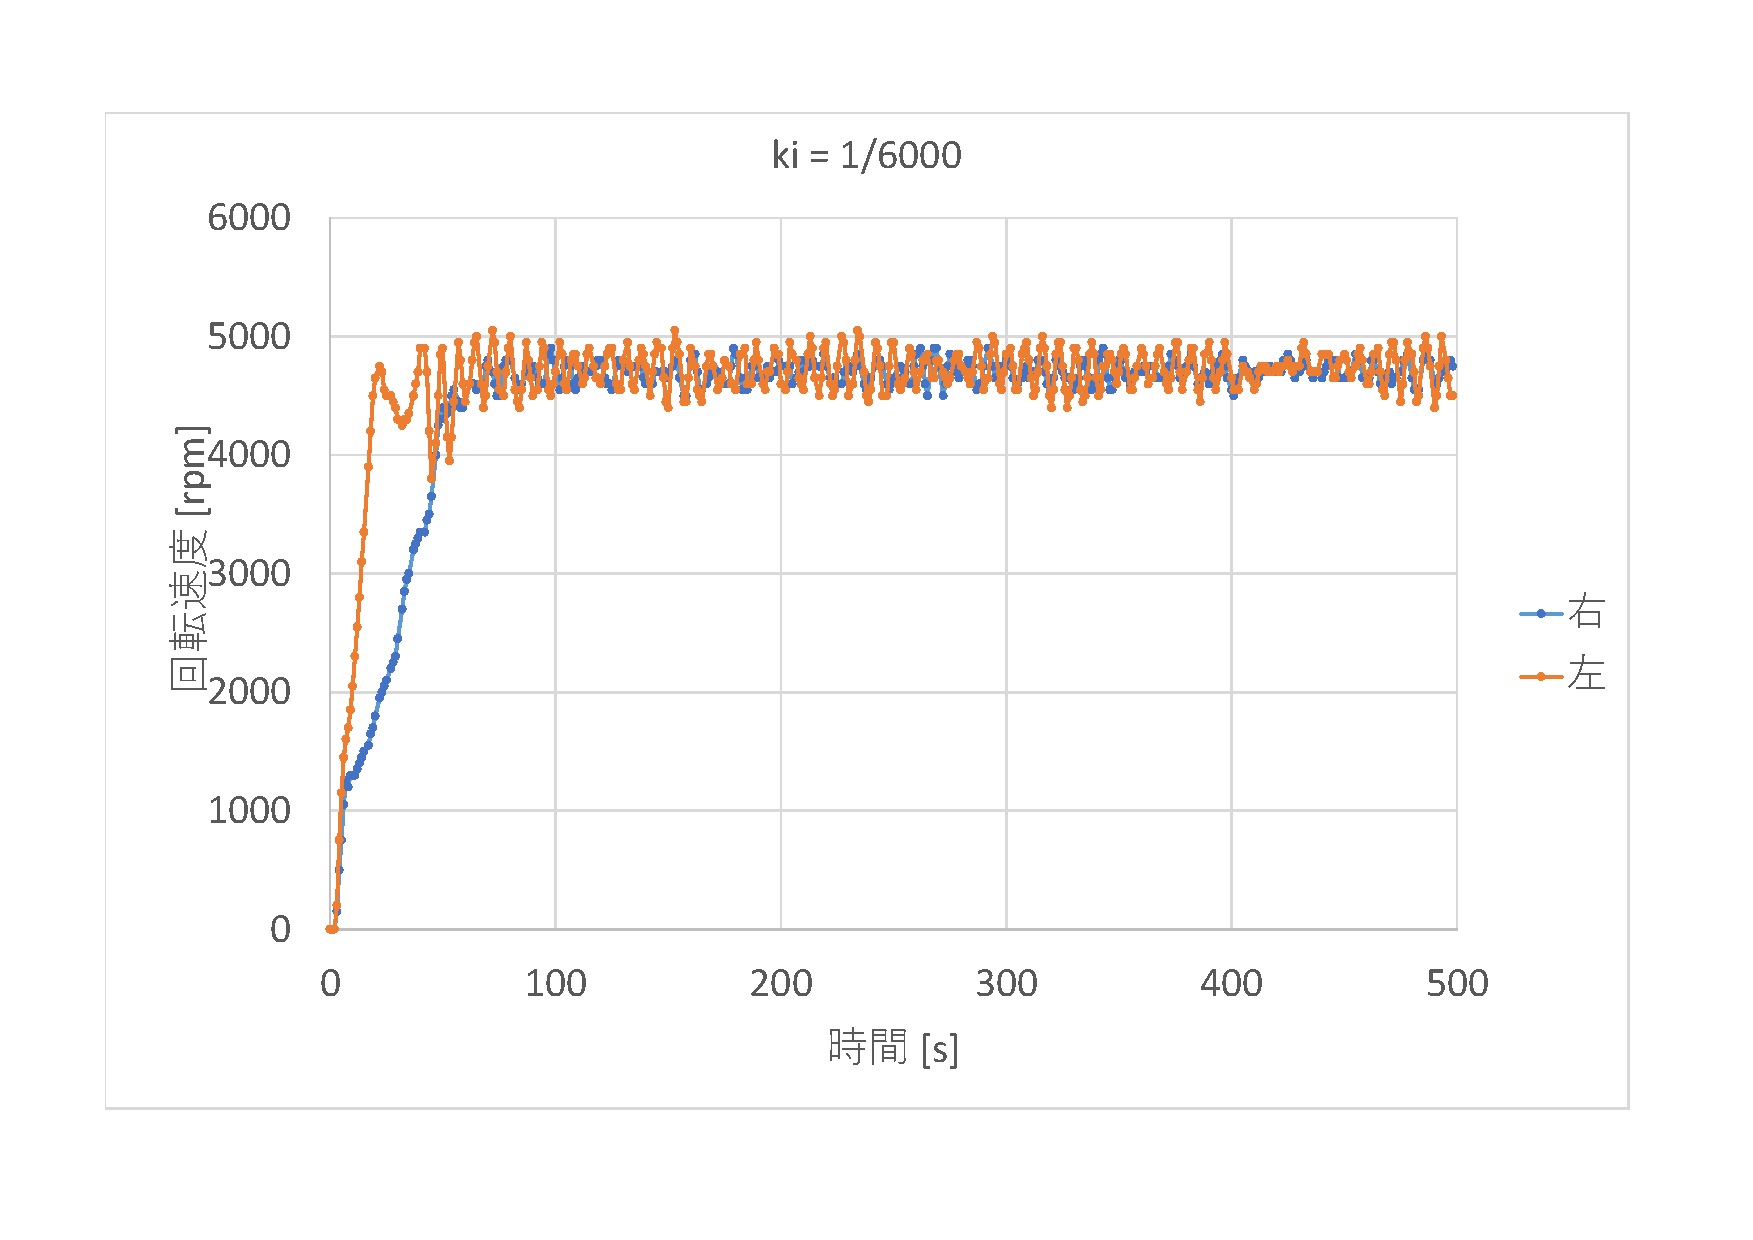
\includegraphics[width=\columnwidth]{img/14/DATA6.pdf}
  \label{im6_14}
  }
  \end{center}
\end{figure}
\begin{figure}[H]
  \begin{center}
  \subfigure[$k_i=1/5000$]{
  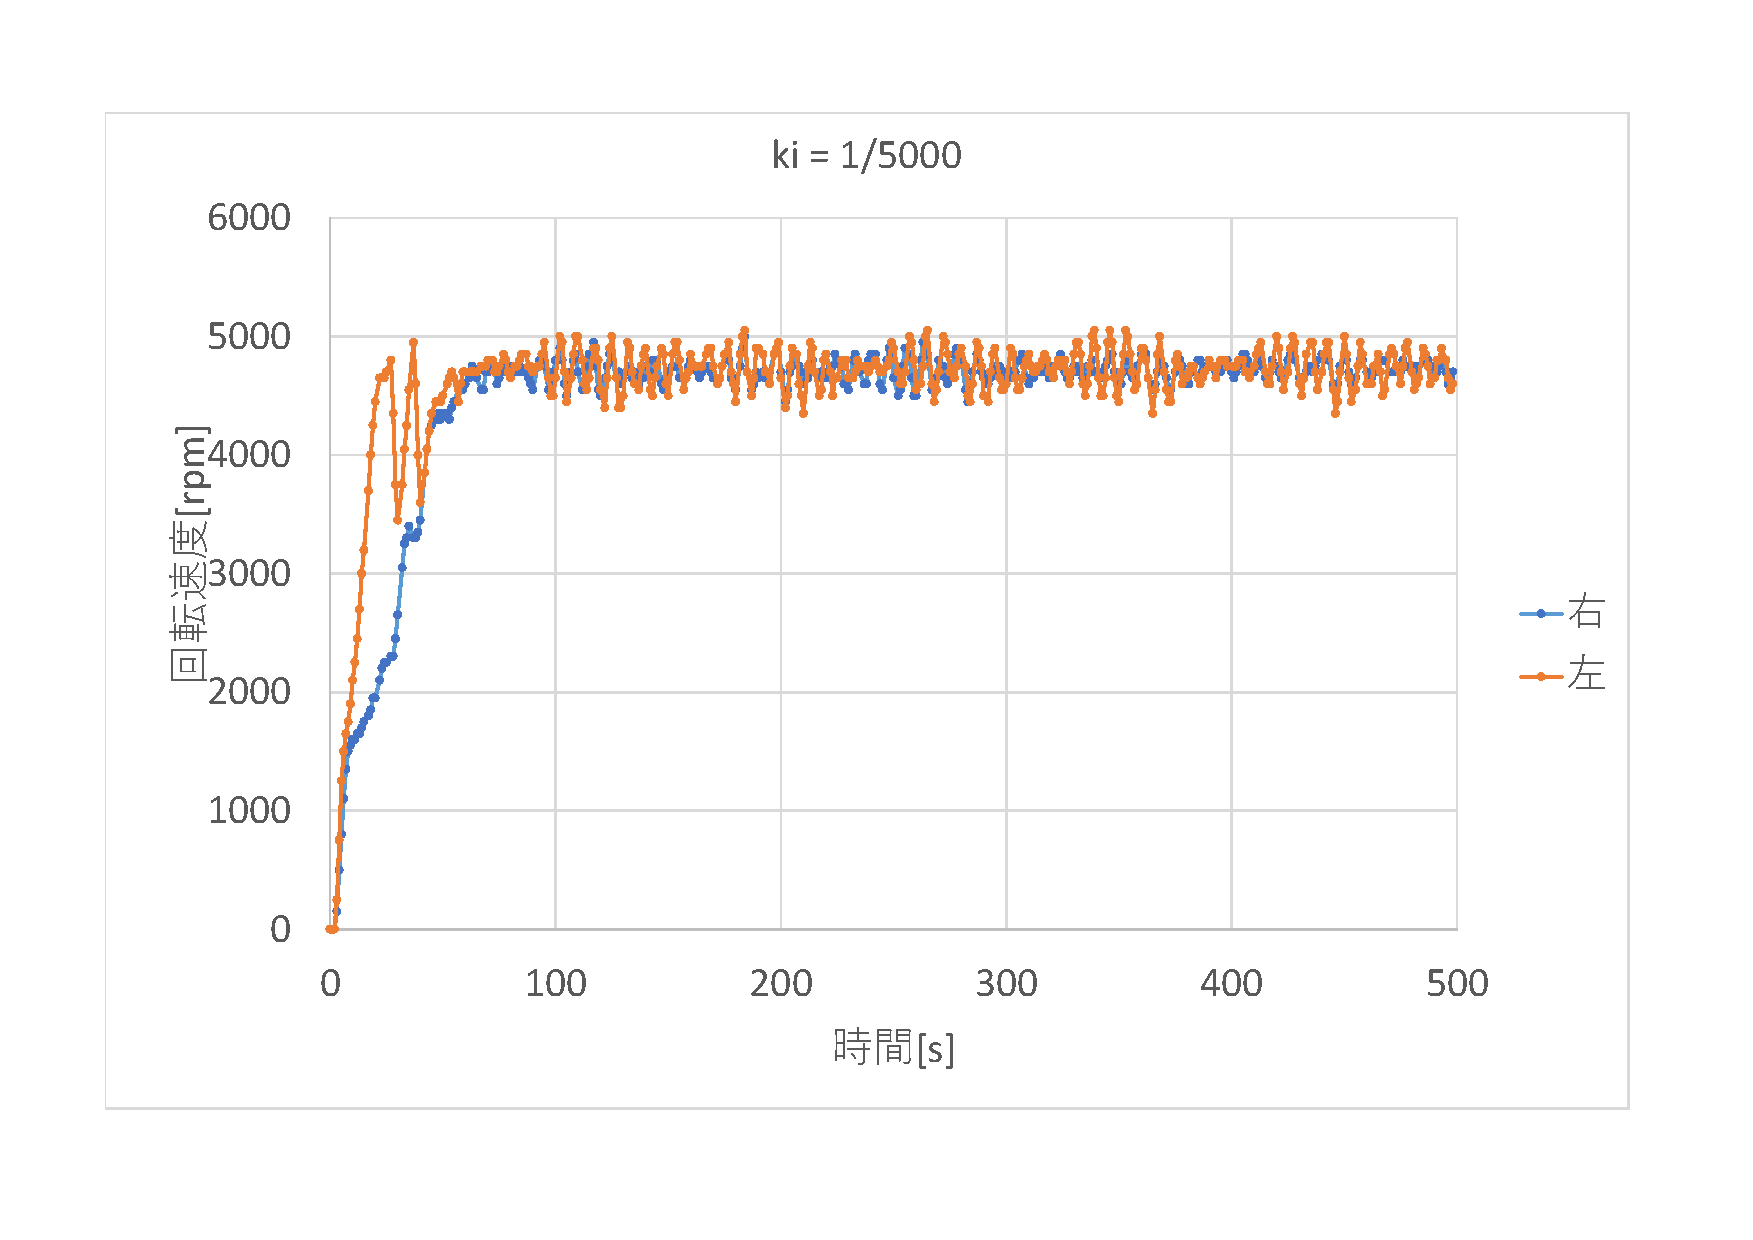
\includegraphics[width=\columnwidth]{img/14/DATA5.pdf}
  \label{im5_14}
  }
  \subfigure[$k_i=1/4000$]{
  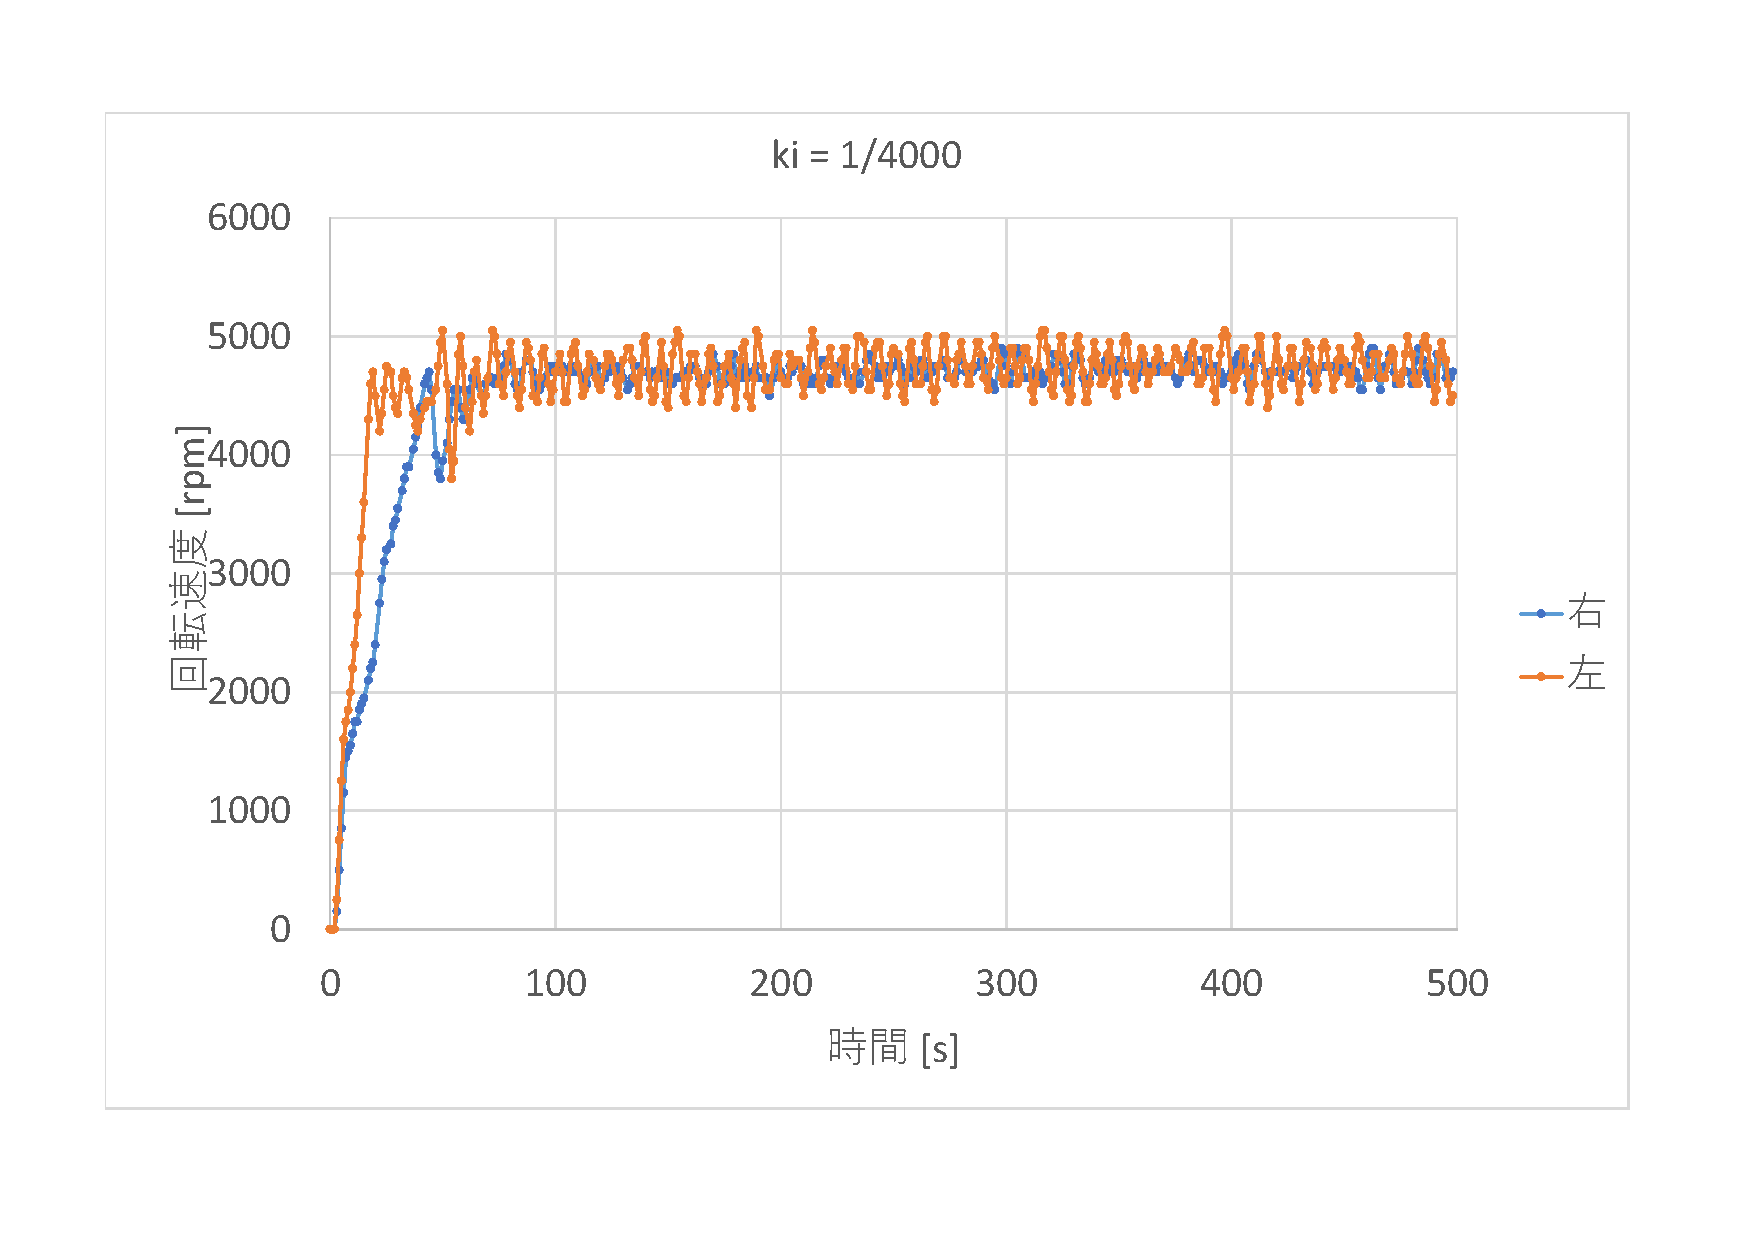
\includegraphics[width=\columnwidth]{img/14/DATA4.pdf}
  \label{im4_14}
  }
  \end{center}
\end{figure}
\begin{figure}[H]
  \begin{center}
  \subfigure[$k_i=1/3000$]{
  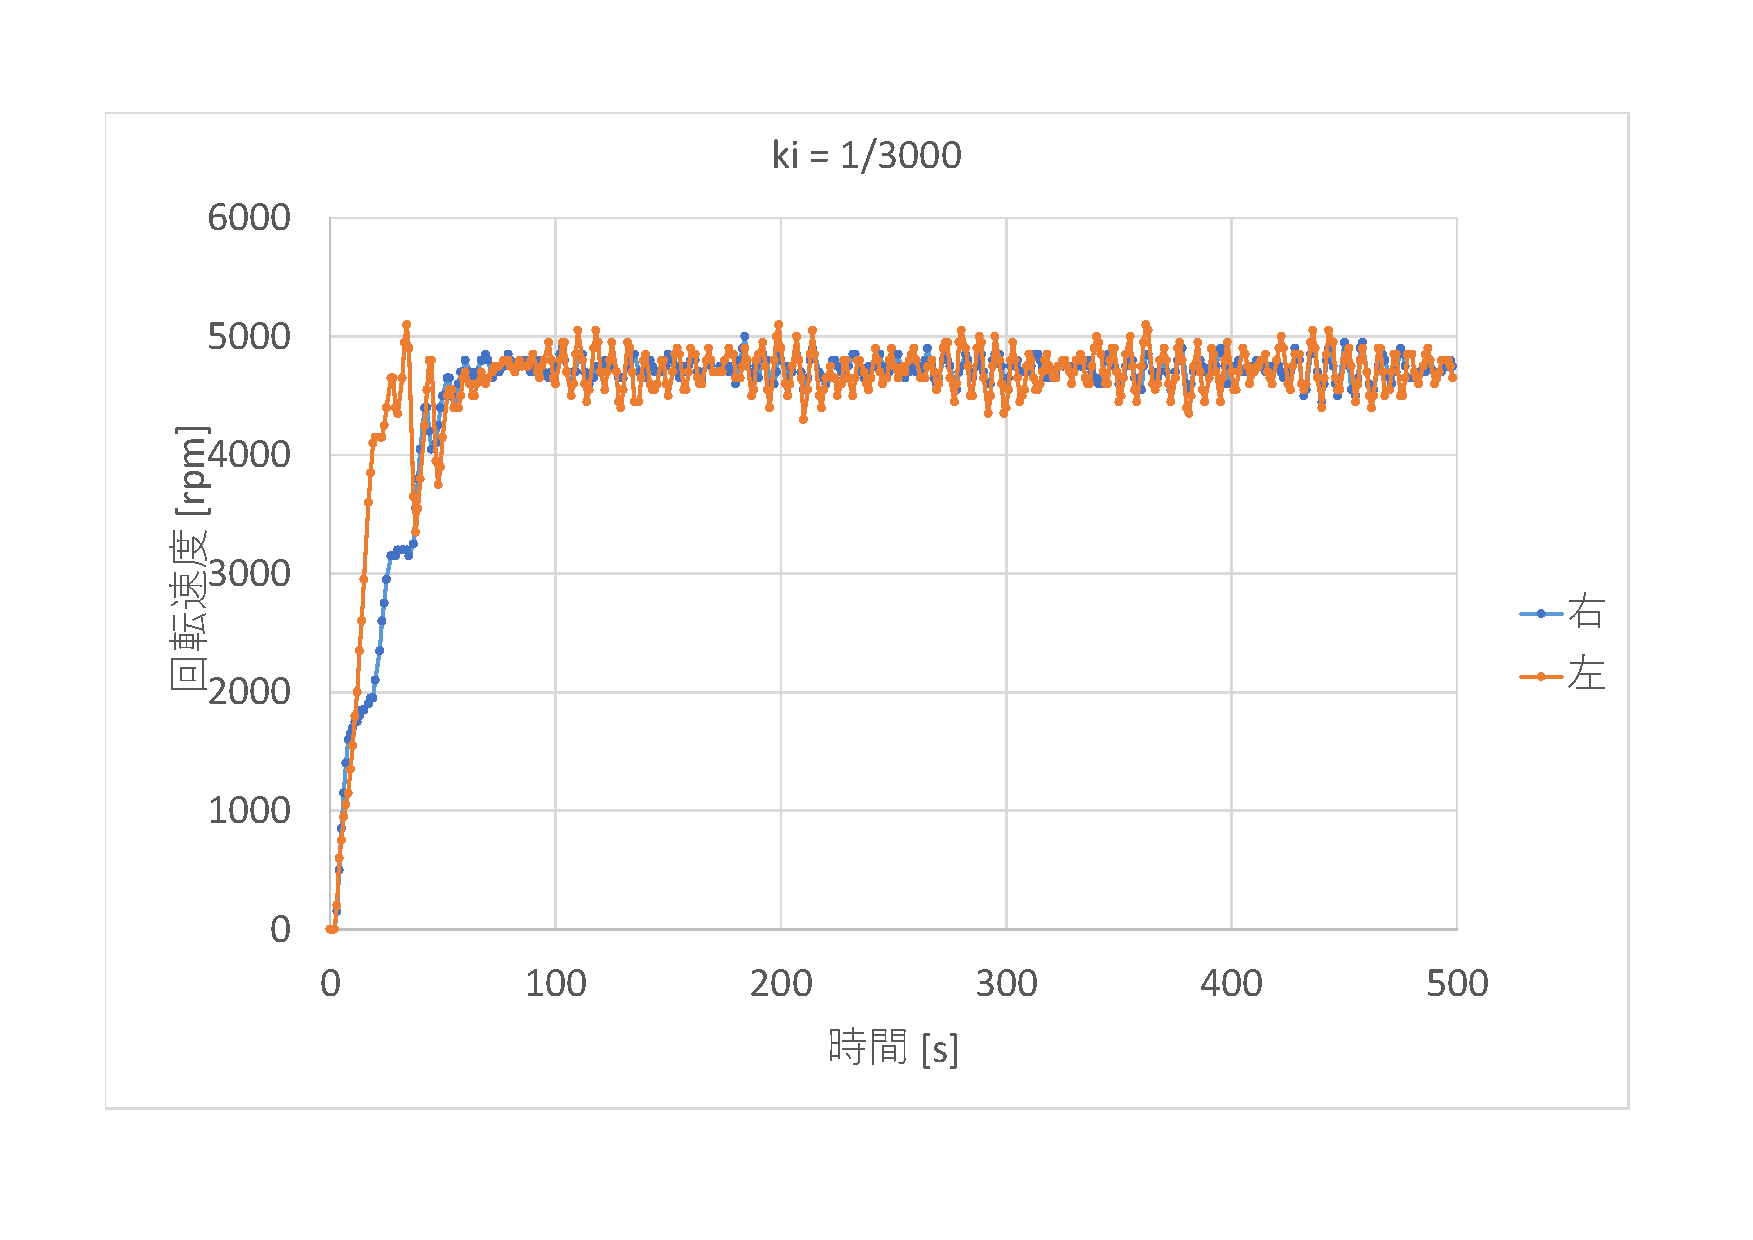
\includegraphics[width=\columnwidth]{img/14/DATA3.pdf}
  \label{im3_14}
  }
  \subfigure[$k_i=1/2000$]{
  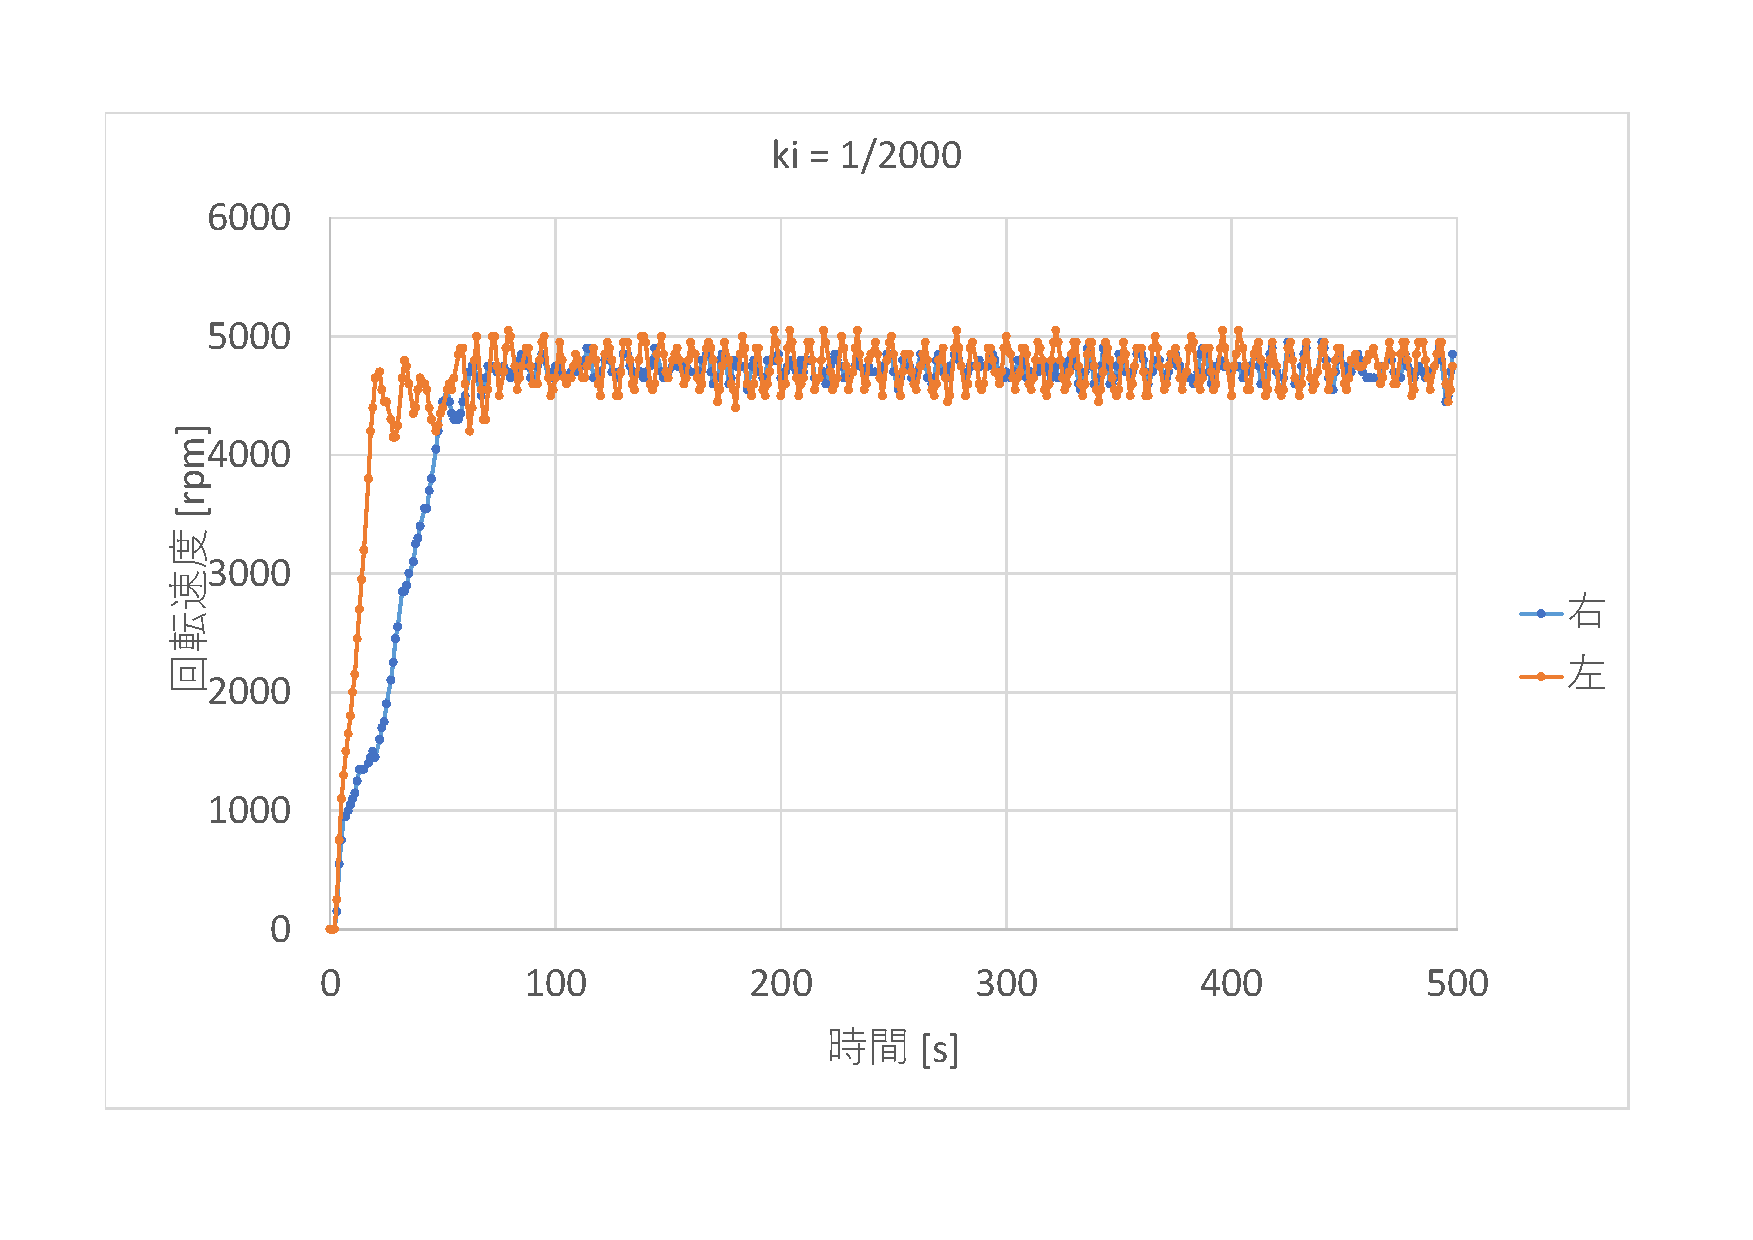
\includegraphics[width=\columnwidth]{img/14/DATA2.pdf}
  \label{im2_14}
  }
  \end{center}
\end{figure}
\begin{figure}[H]
  \begin{center}
  \subfigure[$k_i=1/1000$]{
  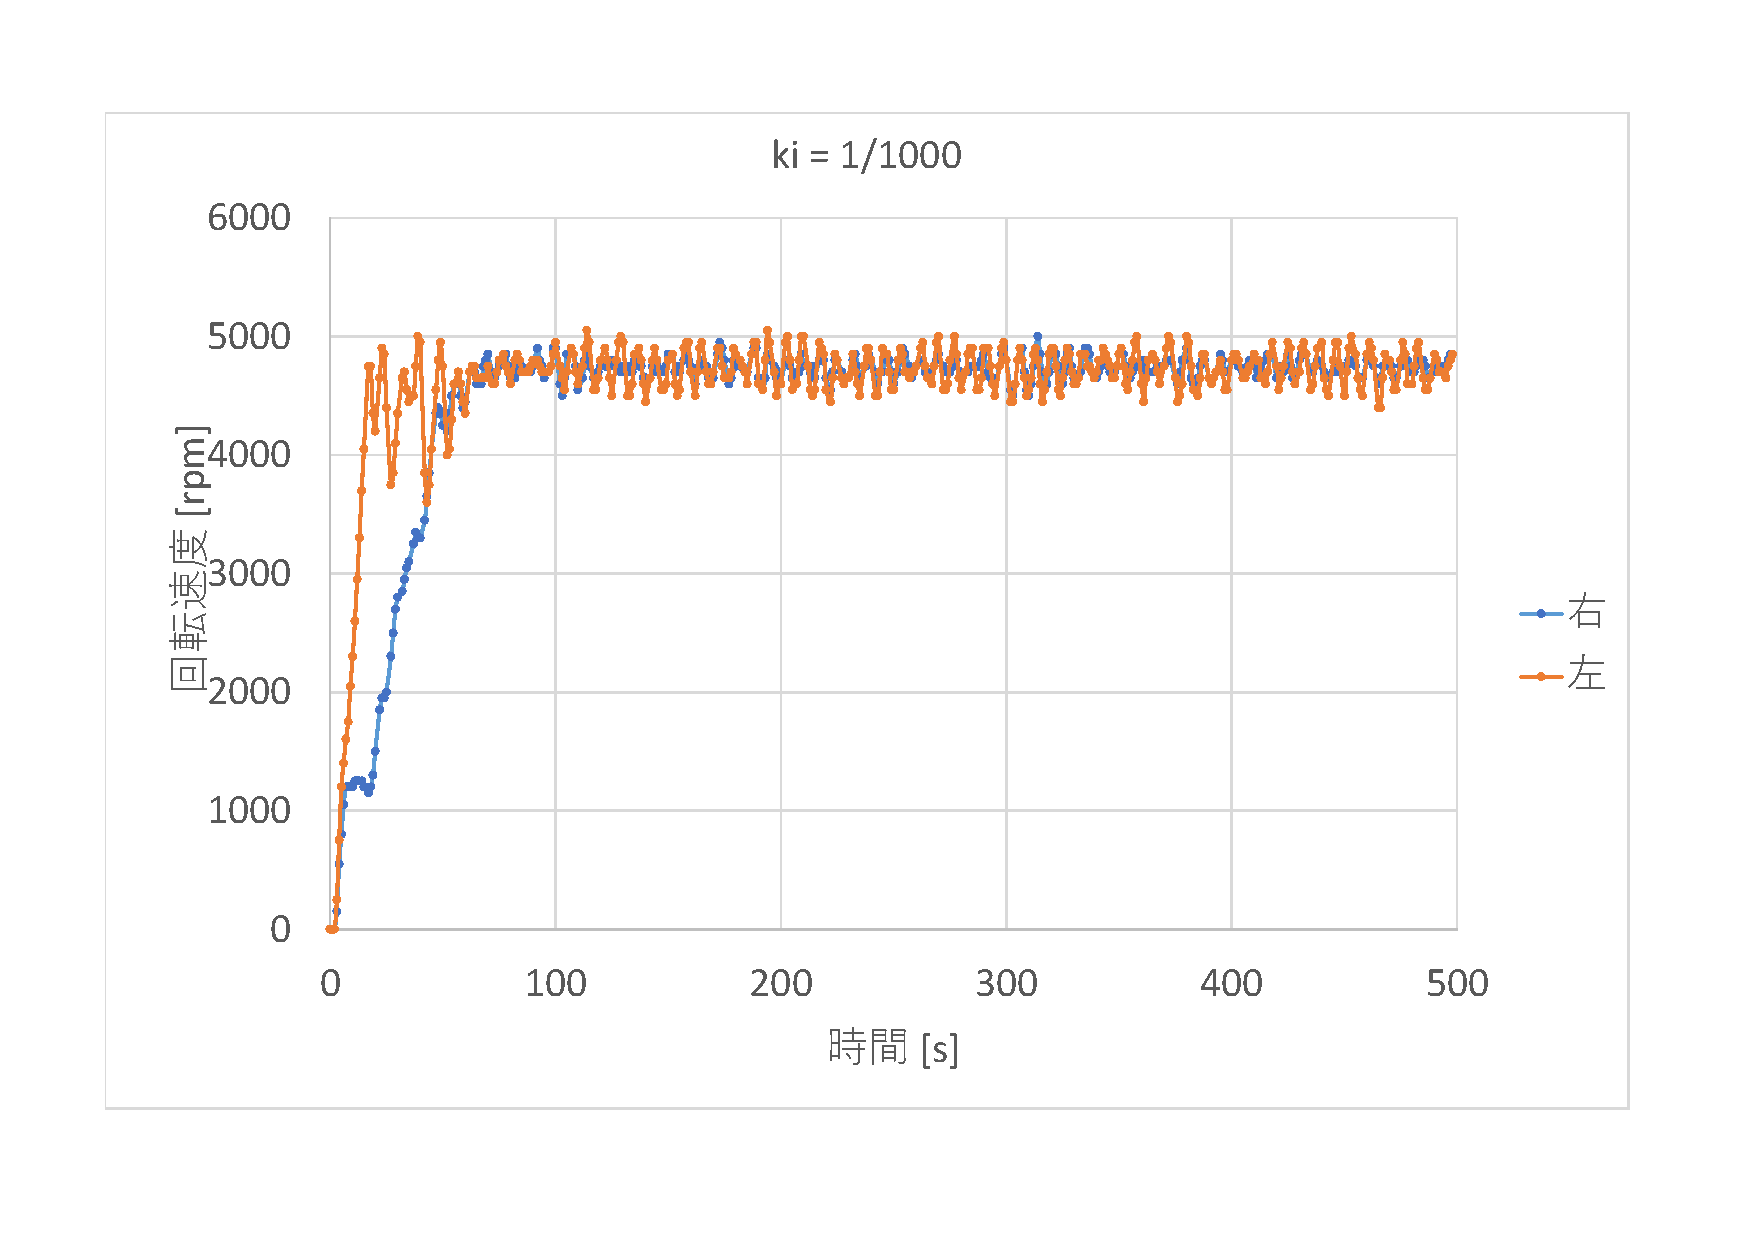
\includegraphics[width=\columnwidth]{img/14/DATA1.pdf}
  \label{im1_14}
  }
  \caption{ステップ応答のグラフ}
  \end{center}
\end{figure}